\section{一维离散映射系统:Logistic映射}
Logistic映射是研究动力系统、混沌、分形等复杂系统的一个经典模型,其来源于生态学中的虫口模型,用以描述种群的变化。Logistic映射从数学形式上来看是一个非常简单的混沌映射,但却有极其复杂的动力学行为,在保密通信领域的应用十分广泛。

Logistic是一个定义在$x\in [0,1]$的一维离散的动力系统,其动力学方程可描述为
\begin{equation}
    x_{n+1}=f(x_n)=\gamma x_n(1-x_n),\ x_n\in [0,1], n=1,2,3,\cdots
\end{equation}
Logistic映射存在两个不动点:$x_1^*=0$和$x_2^*=1-\frac{1}{\gamma}$。Logistic映射的相图描述了相空间的映射关系:
\begin{figure}
	\centering
	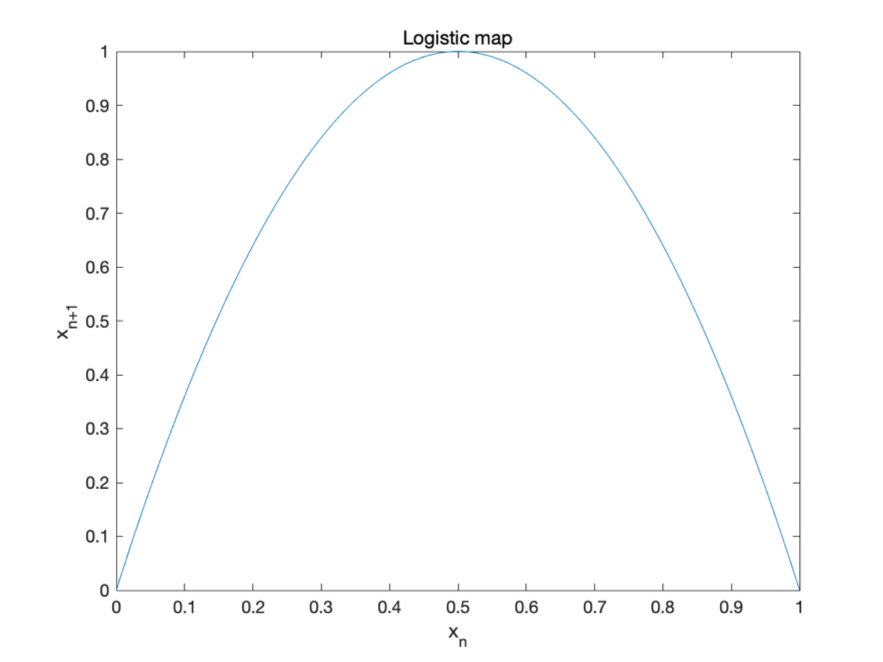
\includegraphics[scale=0.6]{logistic_phase.png}
    \caption{Logistic映射的相图($\gamma=4$)}
    \label{fig:logi_pha}
\end{figure}

Logistic映射的动力学过程可以看作是在一维相空间上的拉伸再折叠的过程。通过非线性动力学的知识可以得到,该系统在$\gamma$取不同值时表现出不同的动力学行为。当$0<\gamma<1$时,系统最终都会渐进的趋于0;当$1<\gamma<3$时,系统会收敛到一个不动点,该不动点的值为$x^*=(\gamma-1)/\gamma$,此时系统的极限行为会趋于该不动点的值;当$3<\gamma<3.57$时,系统的迭代会出现周期行为,随着$\gamma$的增大,周期的长度也会相应的增加,例如2周期,4周期,8周期轨道等,直到大约为$\gamma=3.57$时,周期的长度趋于无穷大;当$3.57<\gamma<4$时,系统的迭代会在周期类型和混沌类型之间来回切换,且大部分区域呈现混沌状态;直到$\gamma=4$时,系统处于完全混沌的状态。

Logistic映射的分岔图$x_n-\gamma$描述了系统随$\gamma$表现出的不同的动力学行为:
\begin{figure}
	\centering
	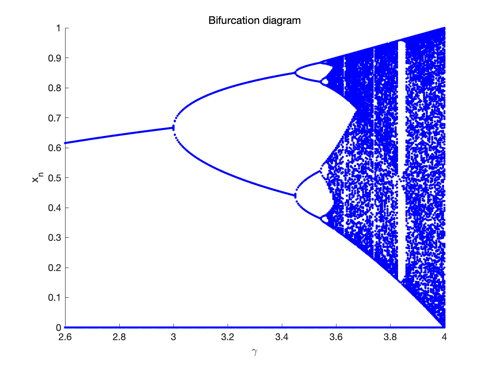
\includegraphics[scale=1]{logistic_bifurcation.png}
    \caption{Logistic映射的分岔图($2.6\leqslant\gamma\leqslant 4$)}
    \label{fig:logi_pha}
\end{figure}

李雅普诺夫指数是描述混沌现象的一个重要的指标,Logistic映射的李雅普诺夫指数图像$\lambda-\alpha$如下图所示:
\begin{figure}
	\centering
	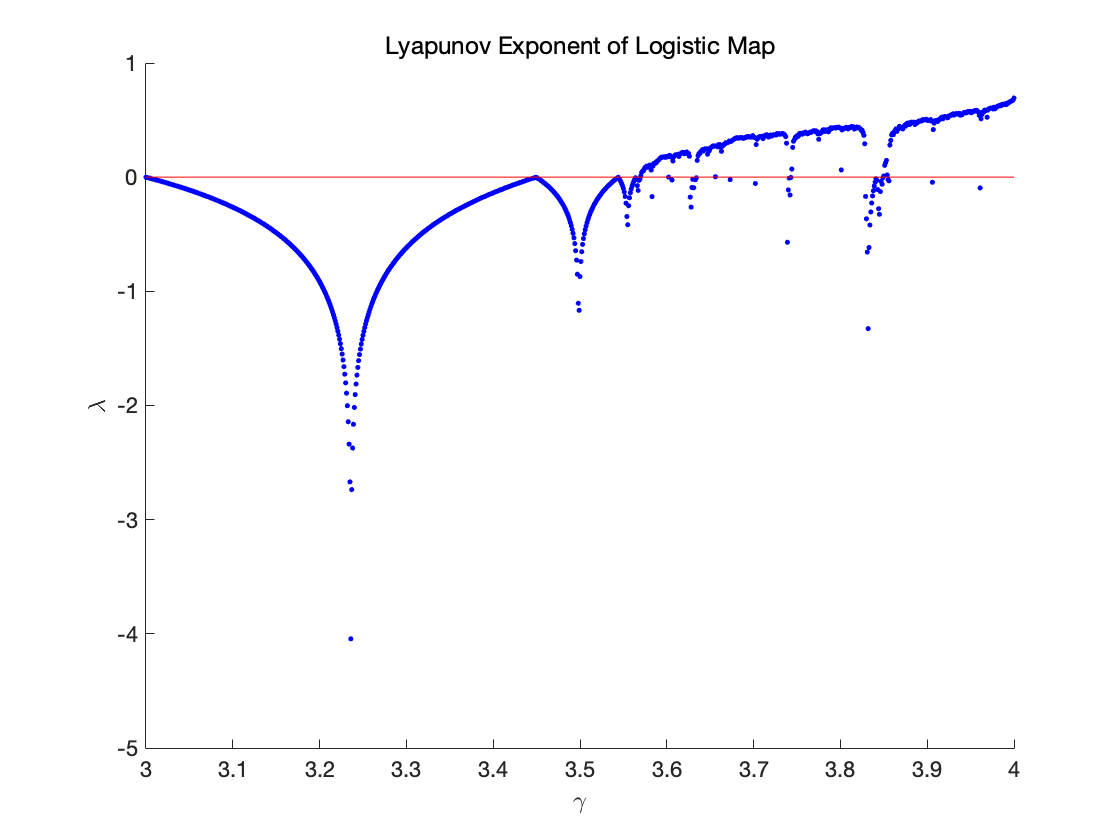
\includegraphics[scale=0.2]{logistic_lypn.png}
    \caption{Logistic映射的李雅普诺夫指数}
    \label{fig:logi_lypn}
\end{figure}
根据李雅普诺夫指数的性质:当$\lambda<0$时,映射系统收敛于某一不动点;当$\lambda=0$时,系统进行周期运动;当$\lambda>0$时,系统处于混沌状态。我们可以同样得到在$3.57<\gamma<4$区域,系统处于混沌状态(在$\gamma=3.83$处存在一三周期轨道),当$\gamma=4$时系统处于混沌状态。

不失一般性,在我们的Koopman分析中,我们取$\gamma=4$的一个特例,通过Logistic映射的动力学方程演化出一系列的数据,作为Koopman分析的源数据,以此来分析Logistic映射的系统特征。

\subsection{Logistic映射的动力学过程}

\subsection{Logistic映射的Koopman算符本征函数}
\subsubsection{正交完备基函数空间}
\begin{figure}
    \centering
    \subfloat[矩形窗基函数]{
      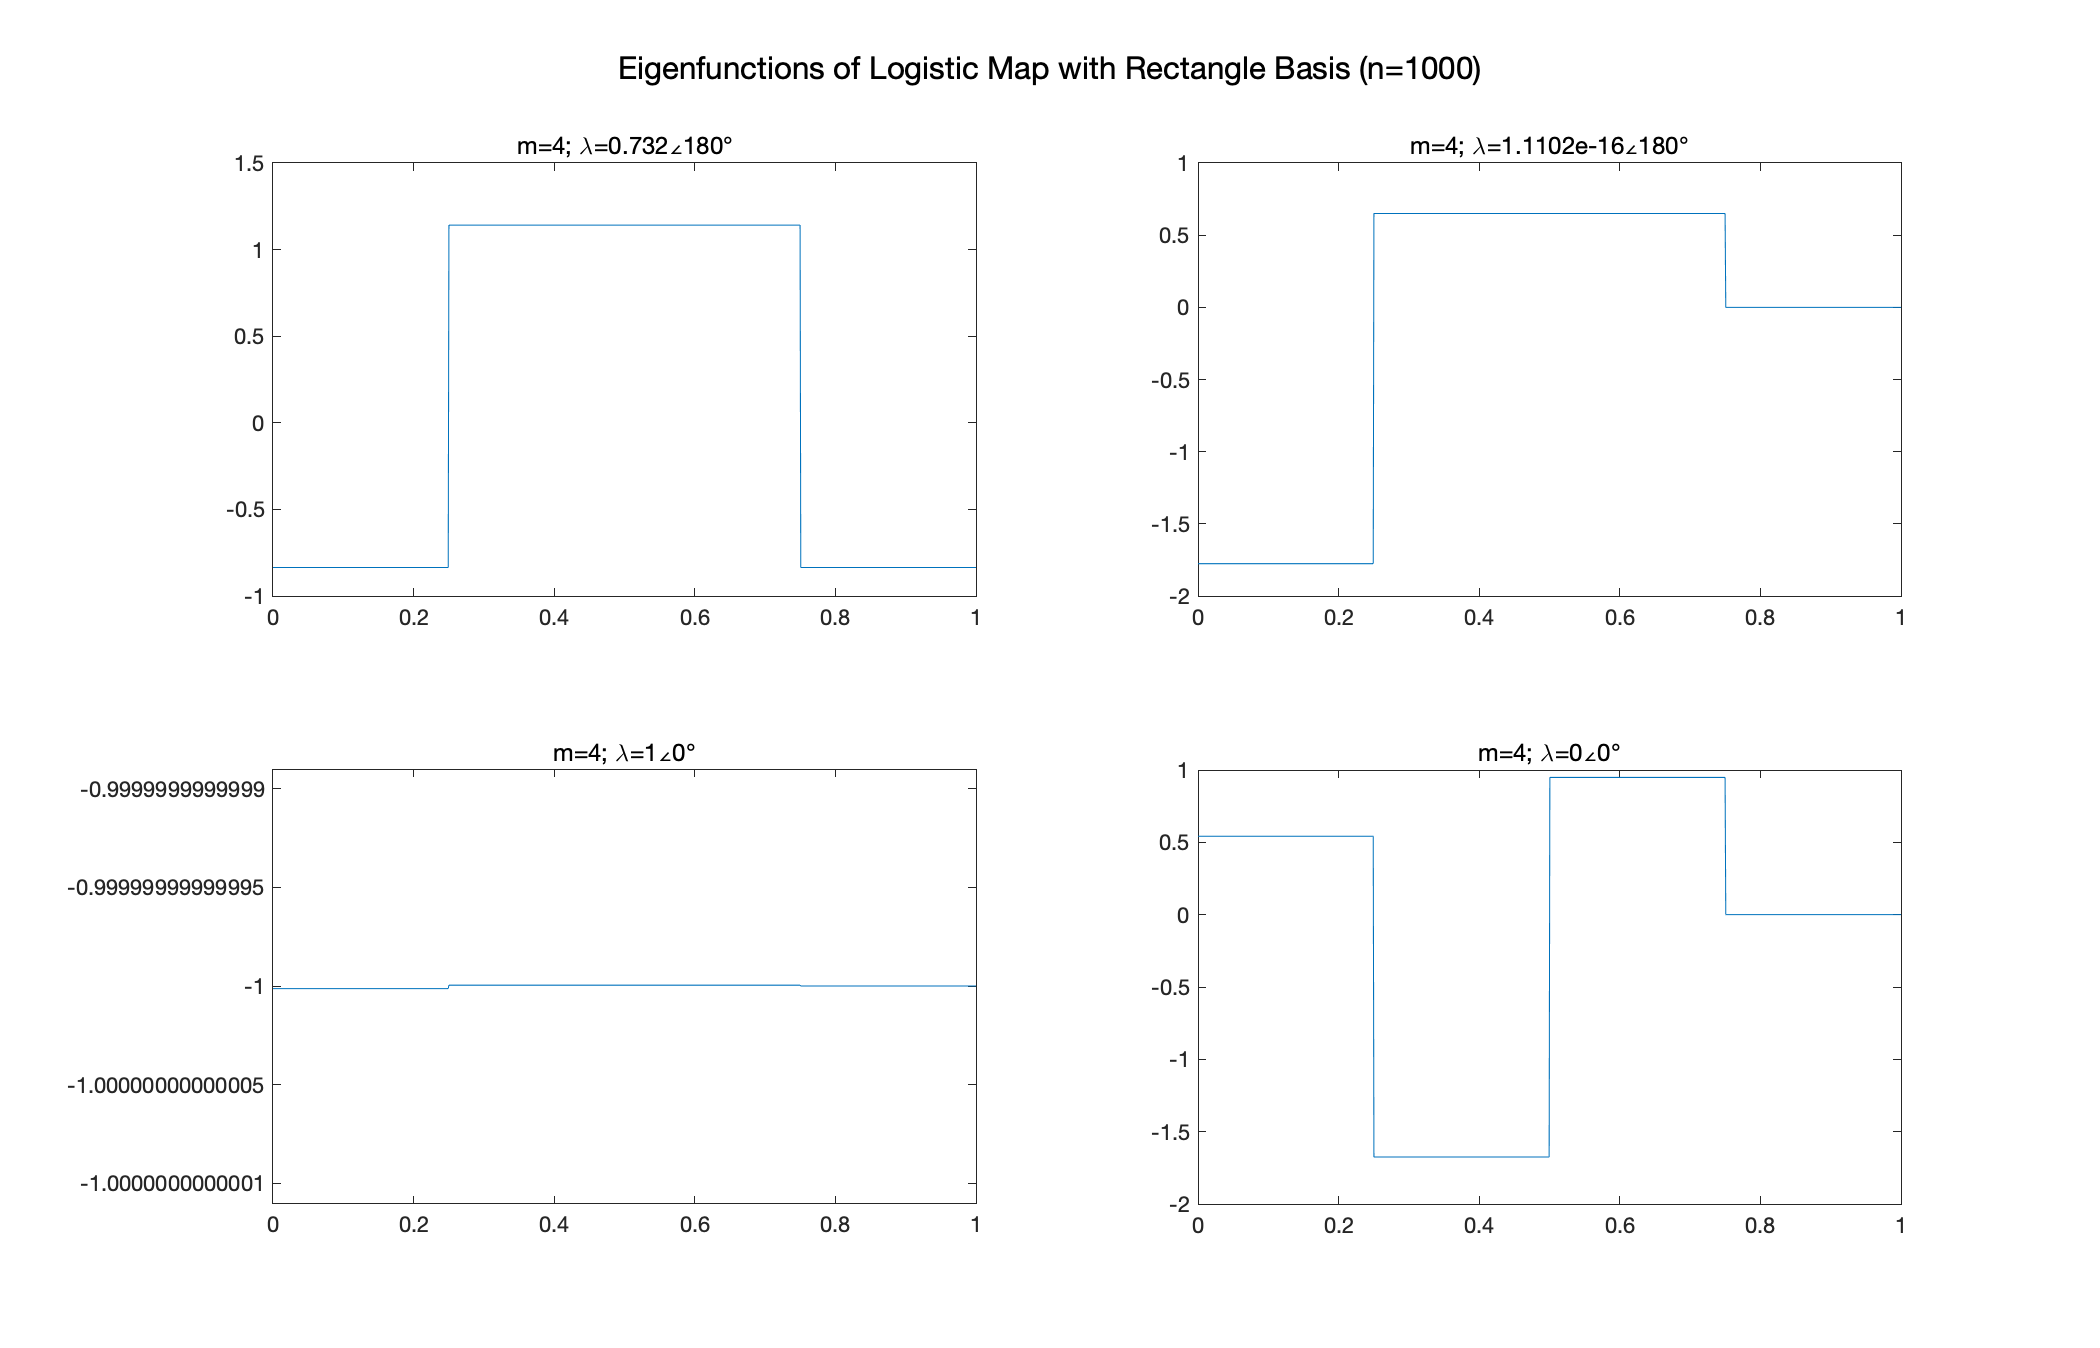
\includegraphics[scale=0.2]{logistic/Logistic_eigen_Rectangle_n1000_m4}}
    \subfloat[高斯基函数]{
      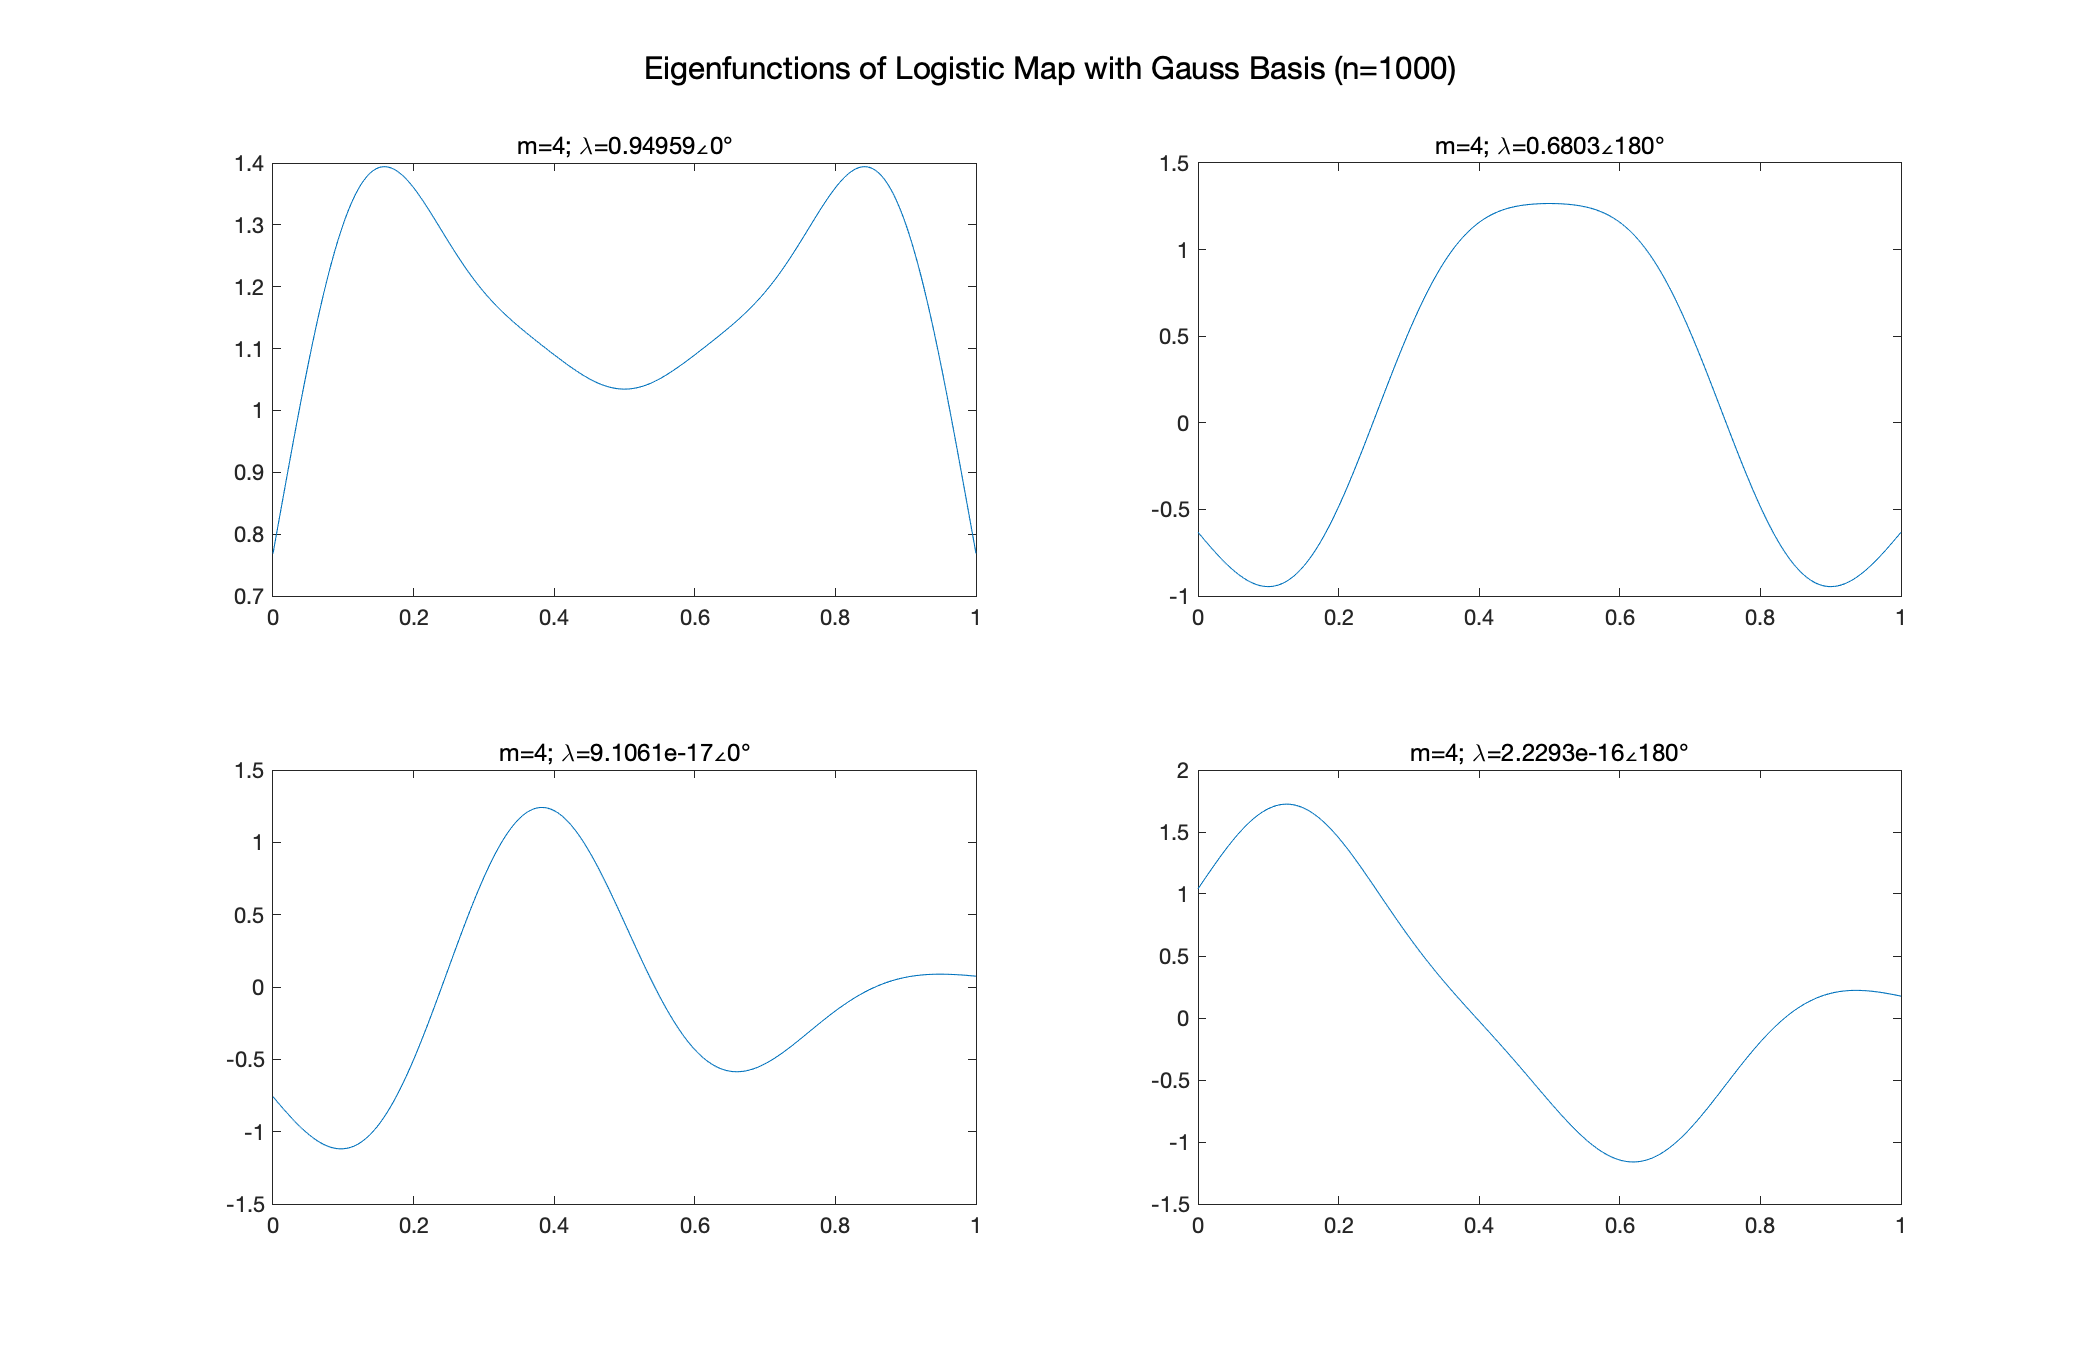
\includegraphics[scale=0.2]{logistic/Logistic_eigen_Gauss_n1000_m4}}
      \\
    \subfloat[傅里叶基函数]{
      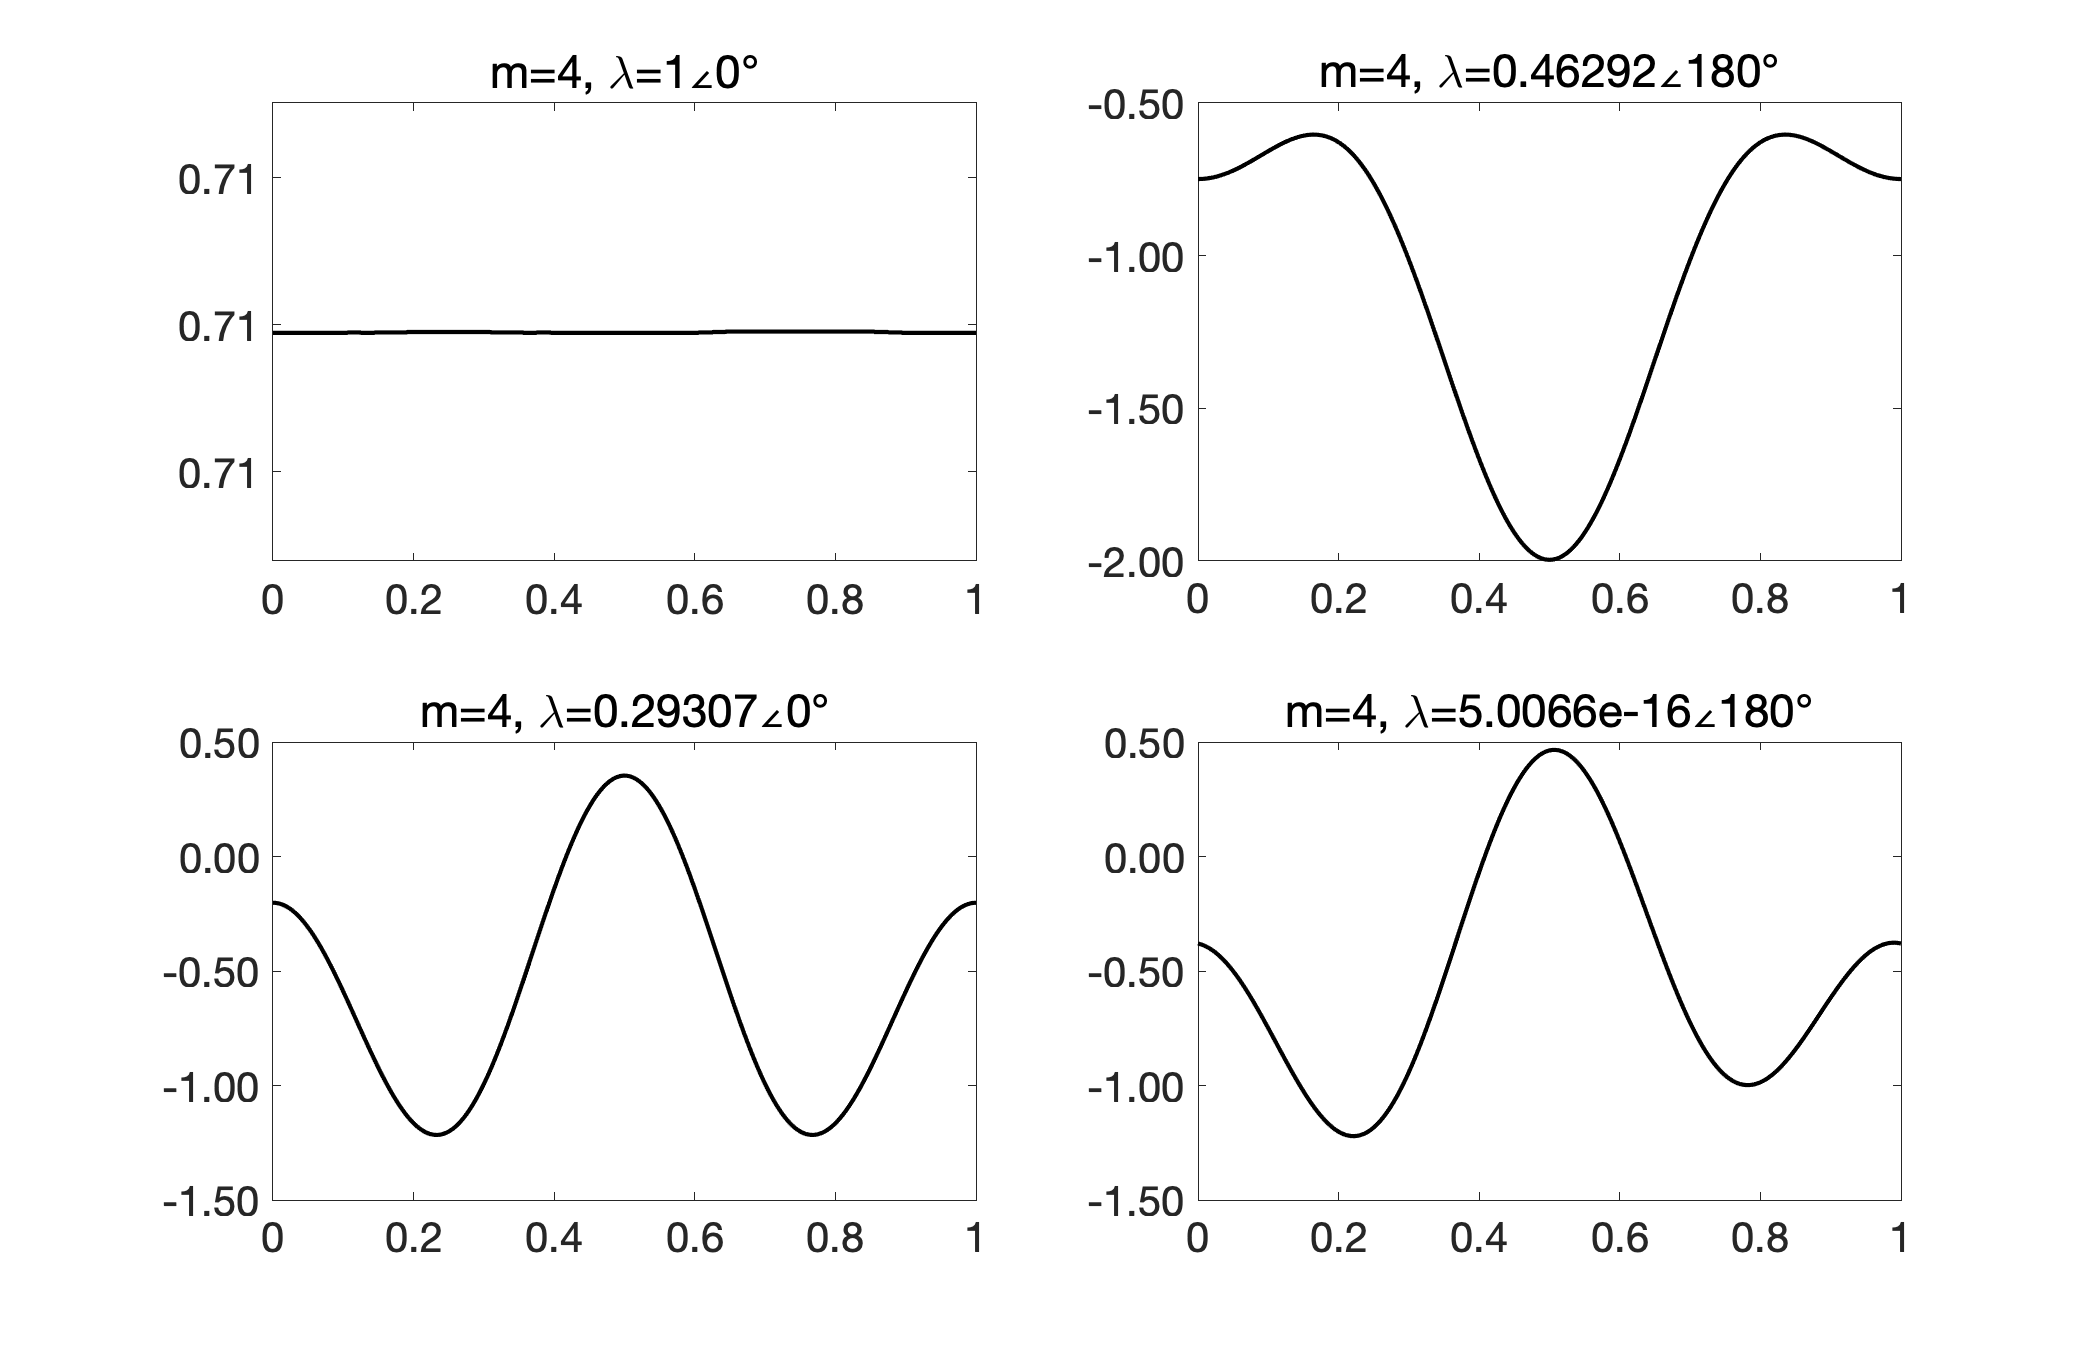
\includegraphics[scale=0.2]{logistic/Logistic_eigen_Fourier_n1000_m4}}
    \subfloat[勒让德基函数]{
      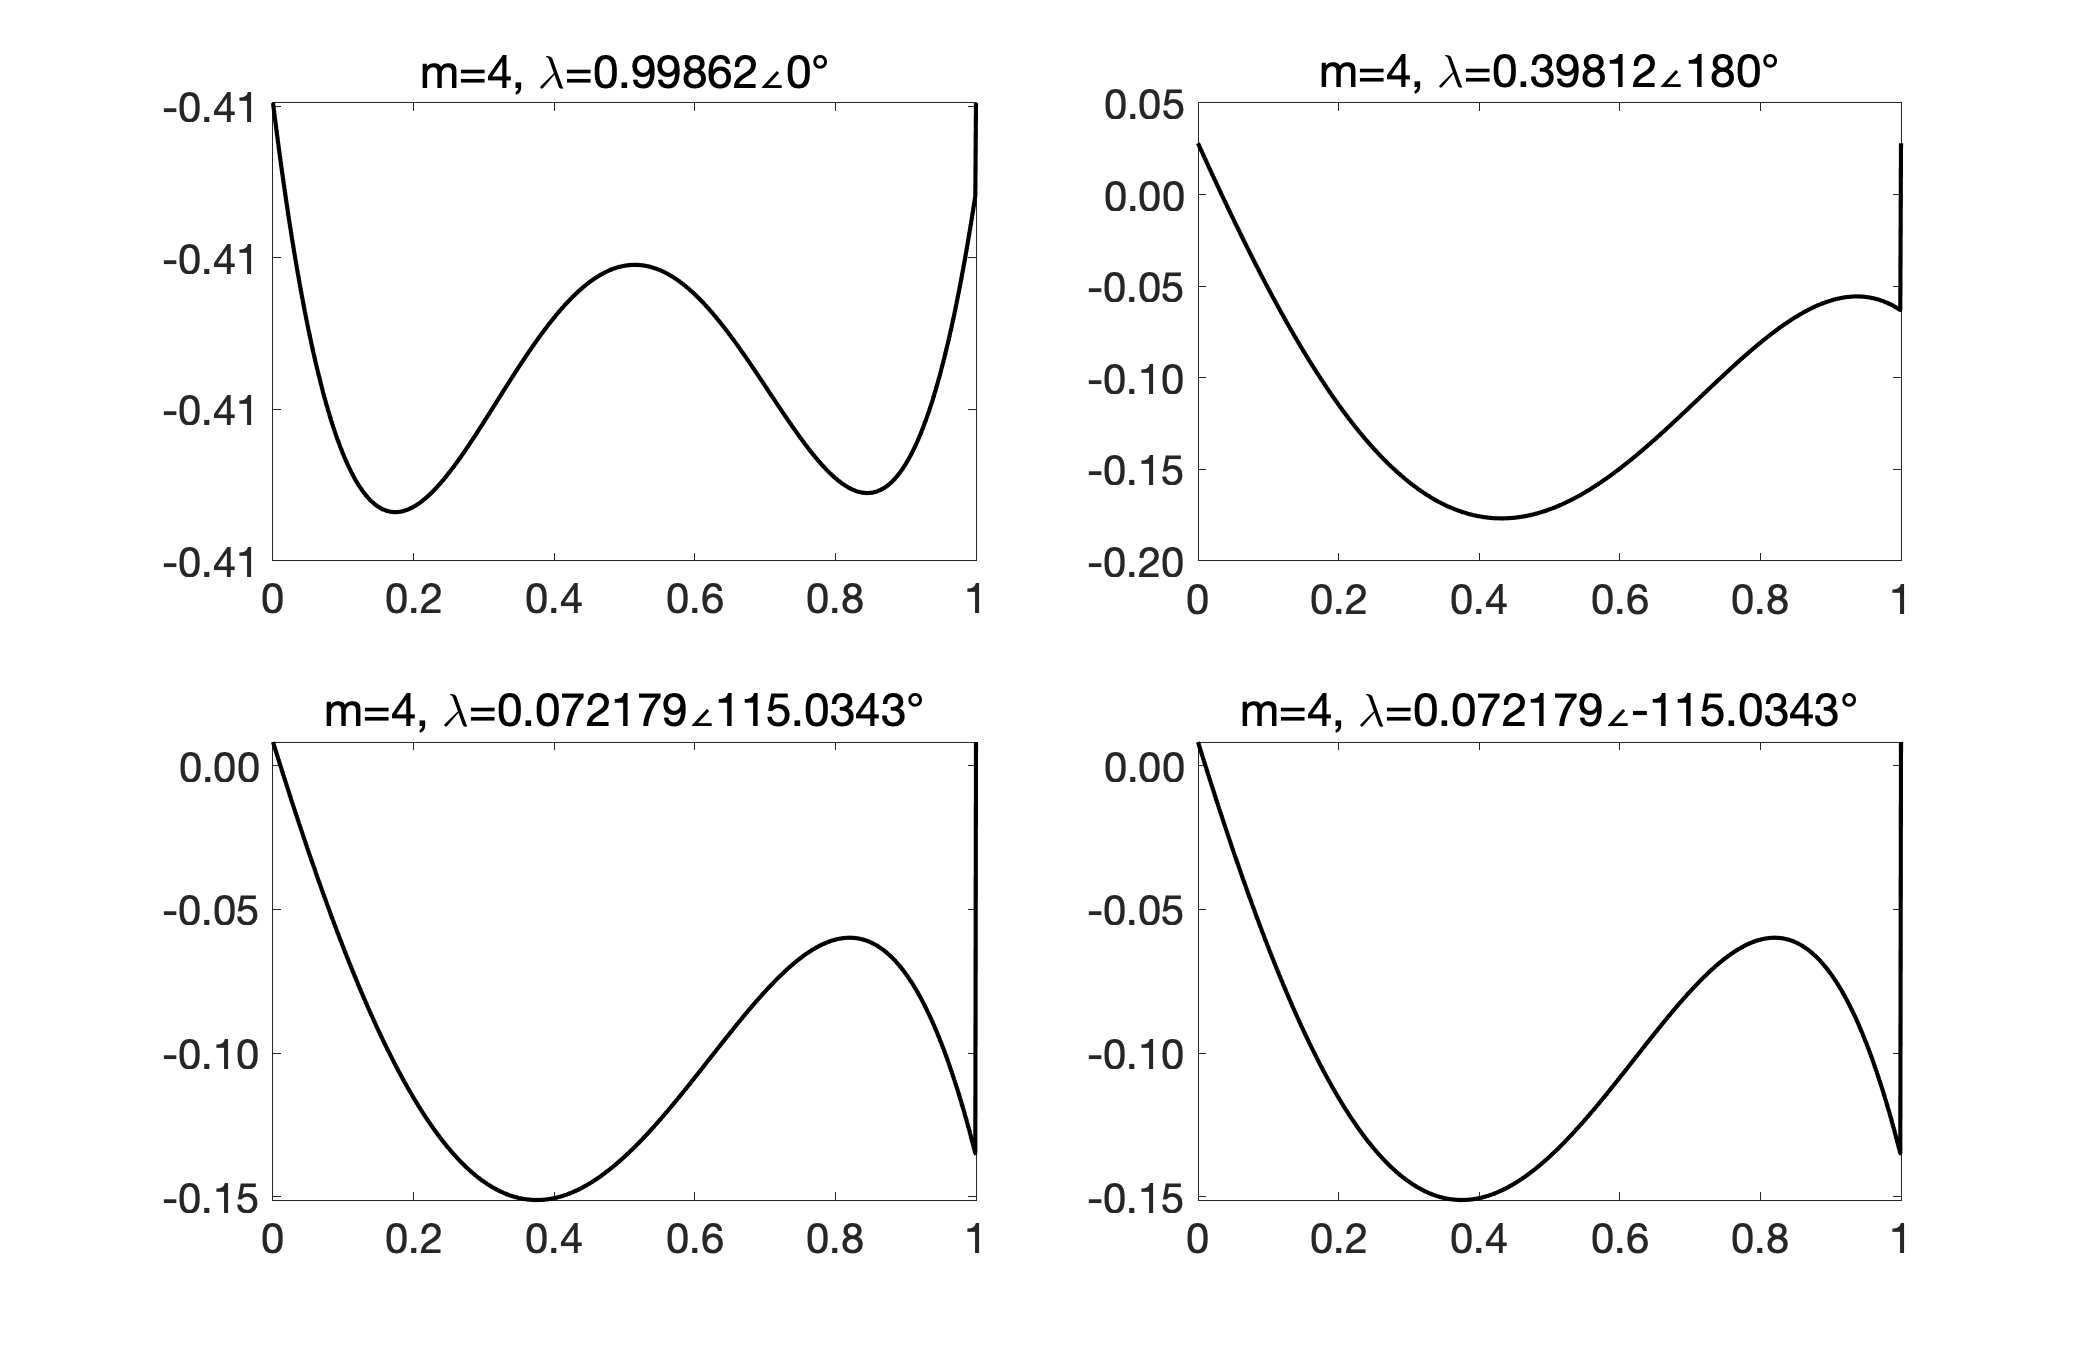
\includegraphics[scale=0.2]{logistic/Logistic_eigen_Legendre_n1000_m4}}
    \caption{四种基函数下Logistic映射的本征函数($m=4$)}
\end{figure}
\begin{figure}
  \centering
  \subfloat[矩形窗基函数]{
    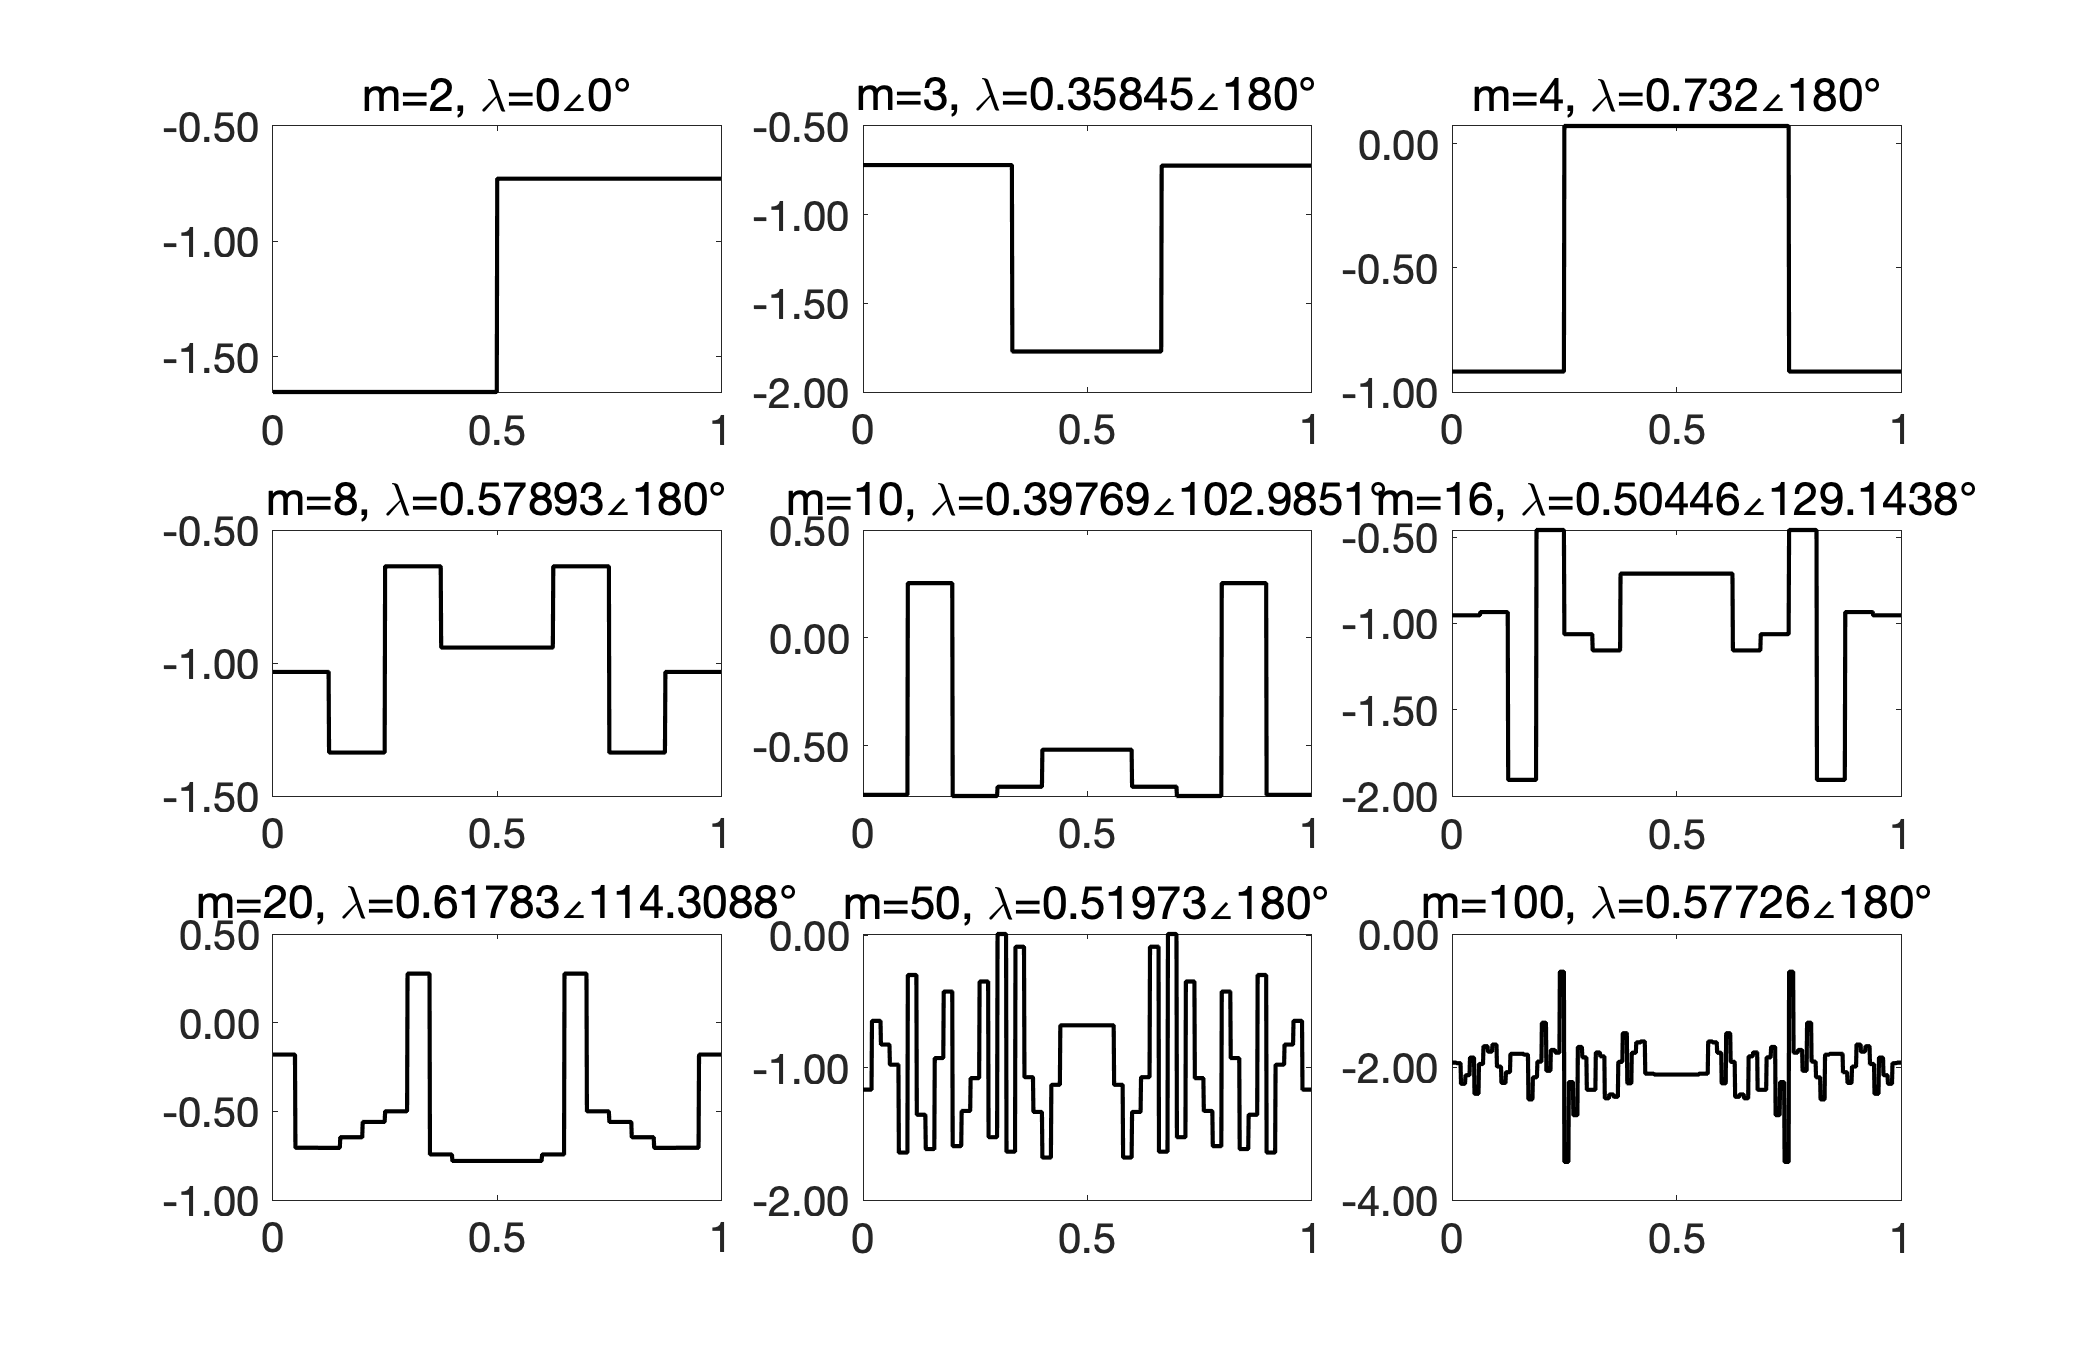
\includegraphics[scale=0.2]{logistic/Logistic_eigen_Rectangle_n1000_m2-3-4-8-10-16-20-50-100}}
  \subfloat[高斯基函数]{
    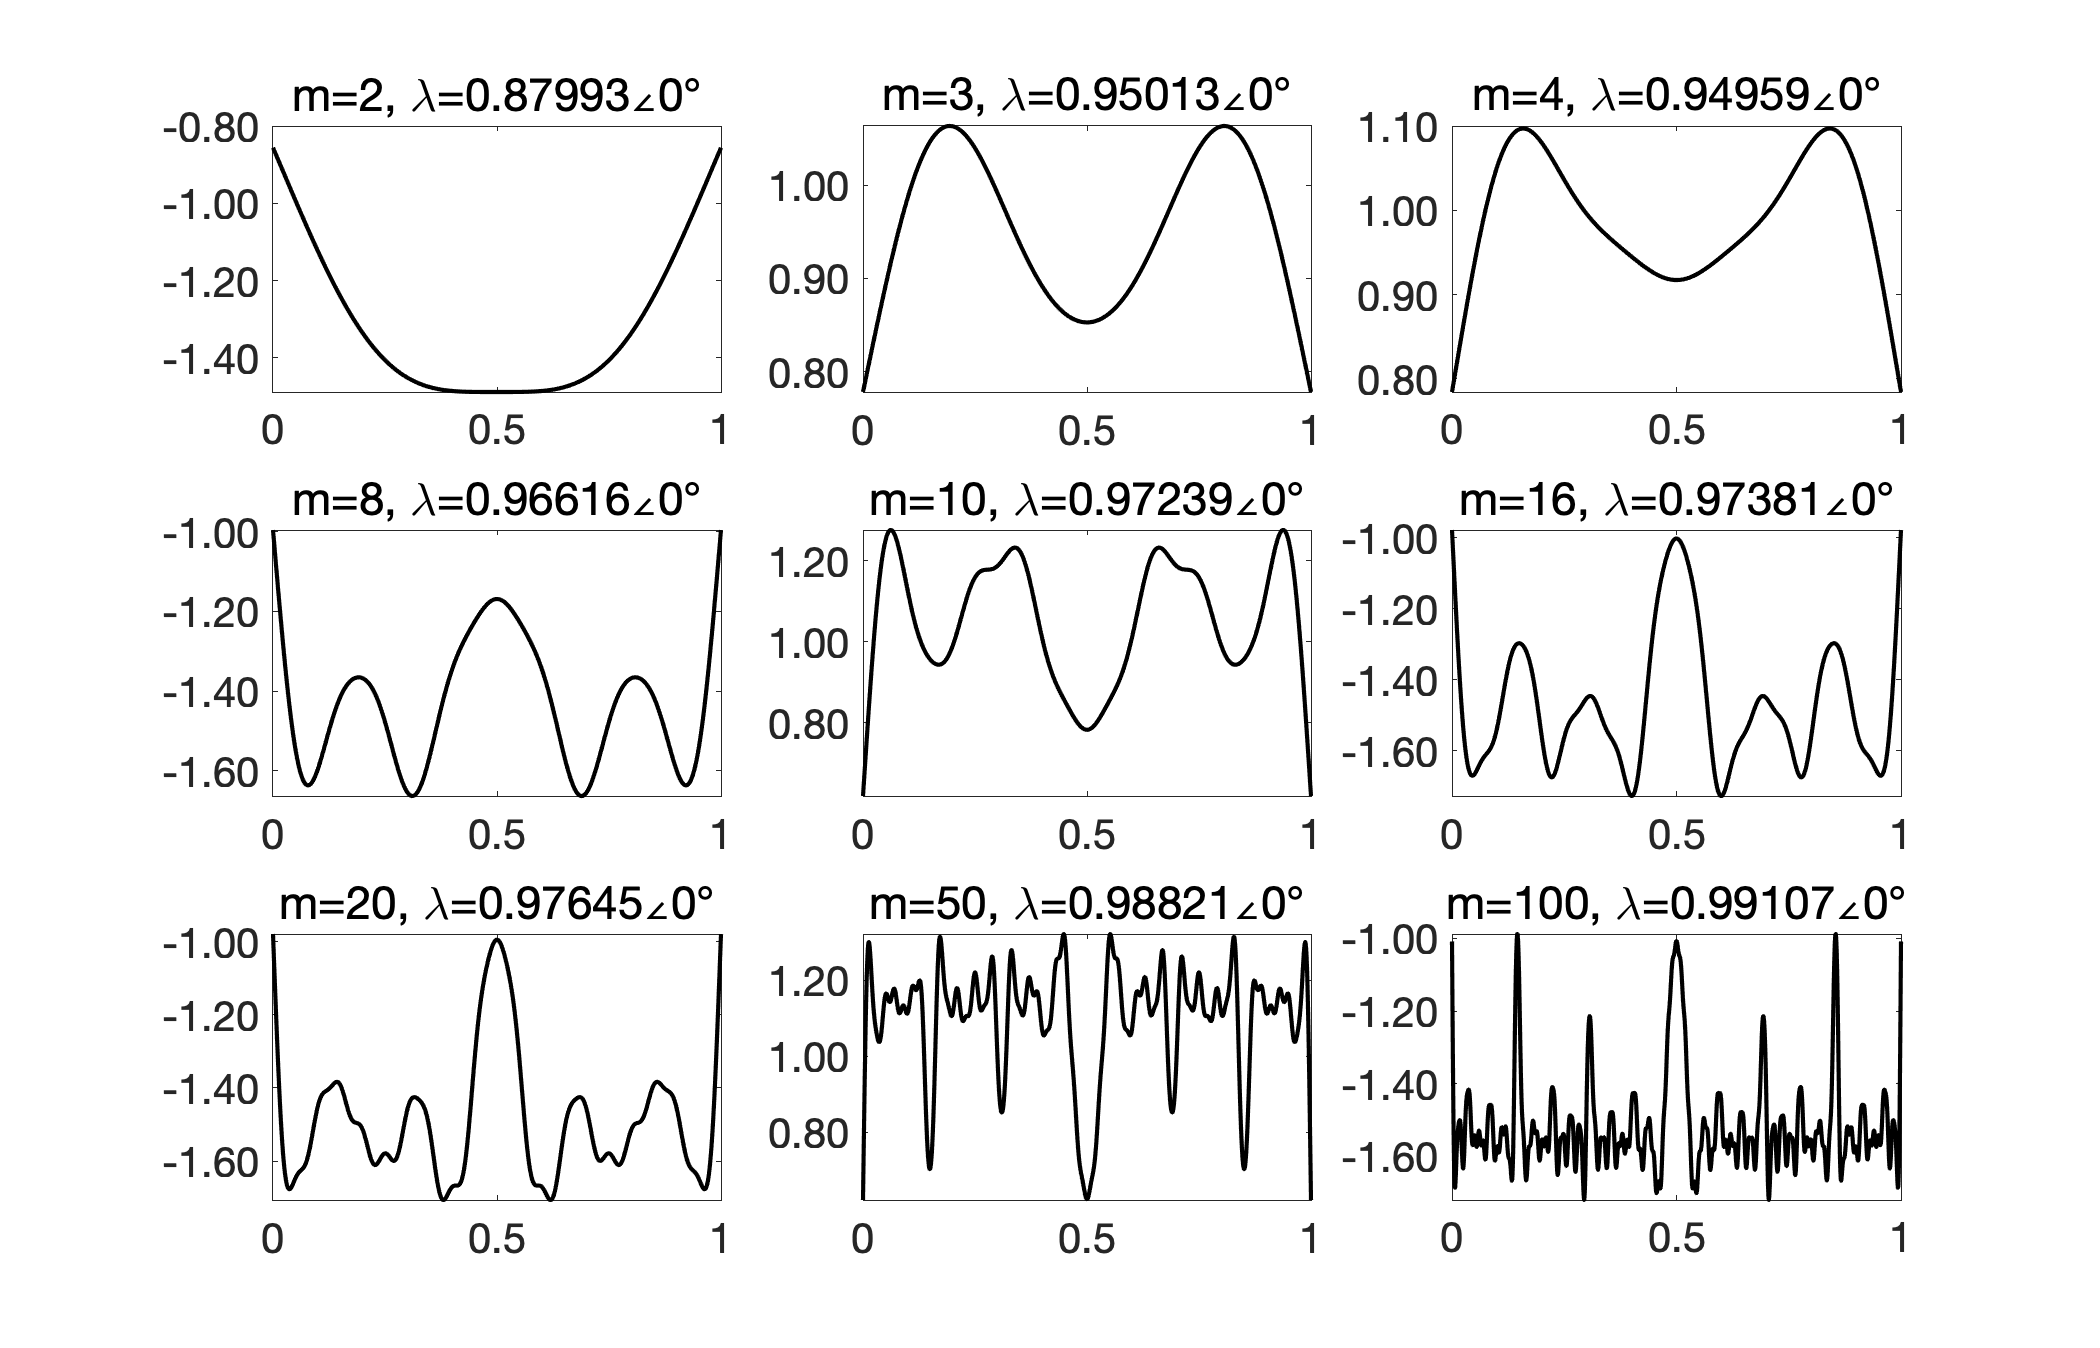
\includegraphics[scale=0.2]{logistic/Logistic_eigen_Gauss_n1000_m2-3-4-8-10-16-20-50-100}}
    \\
  \subfloat[傅里叶基函数]{
    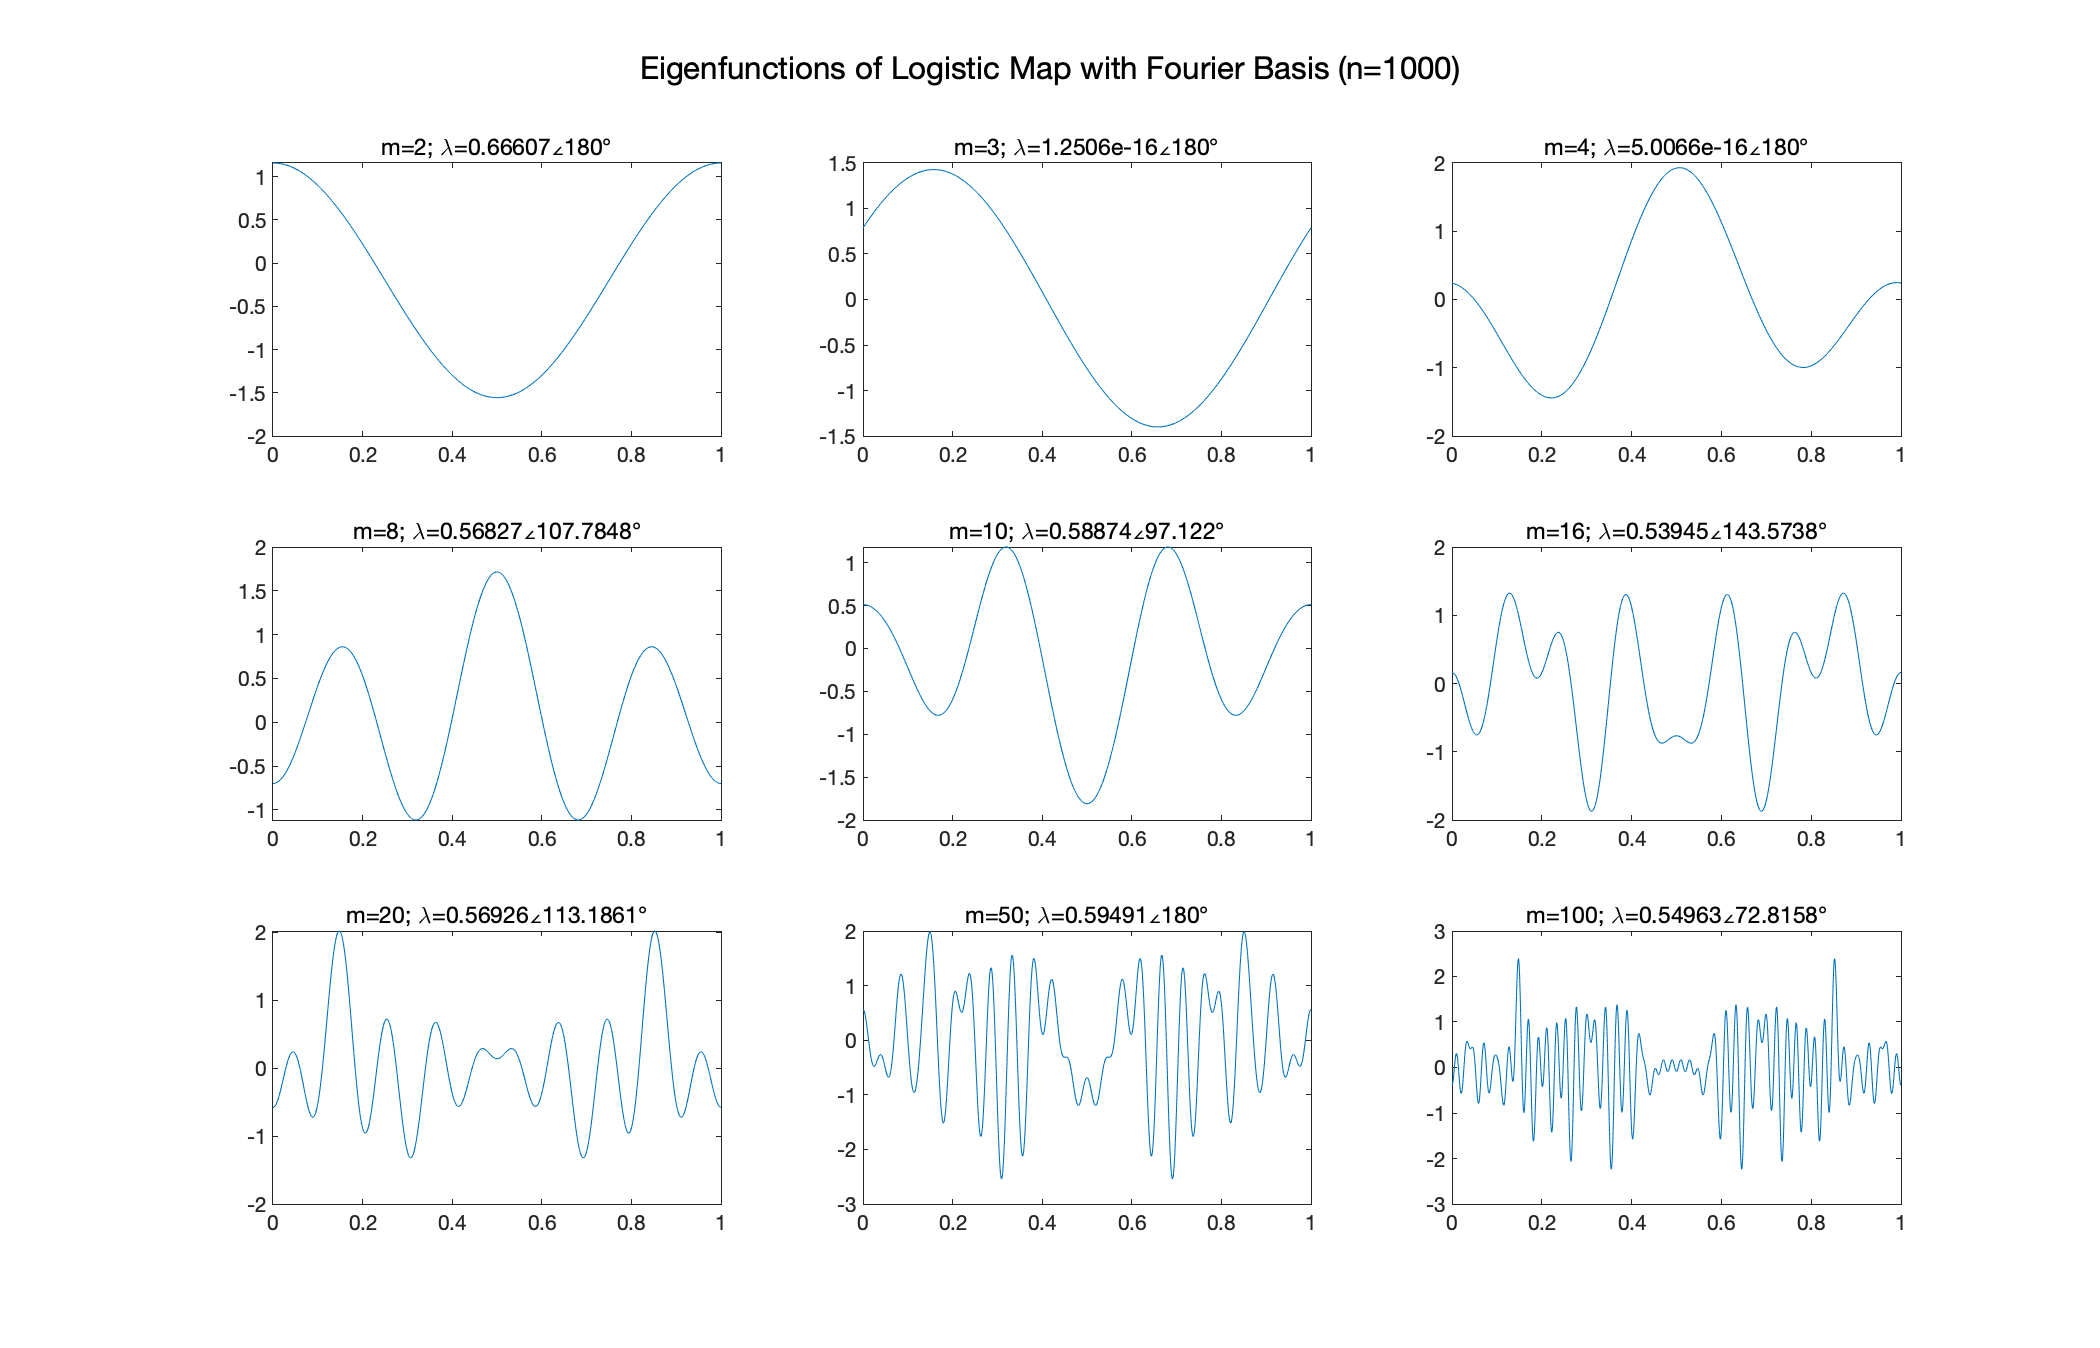
\includegraphics[scale=0.2]{logistic/Logistic_eigen_Fourier_n1000_m2-3-4-8-10-16-20-50-100}}
  \subfloat[勒让德基函数]{
    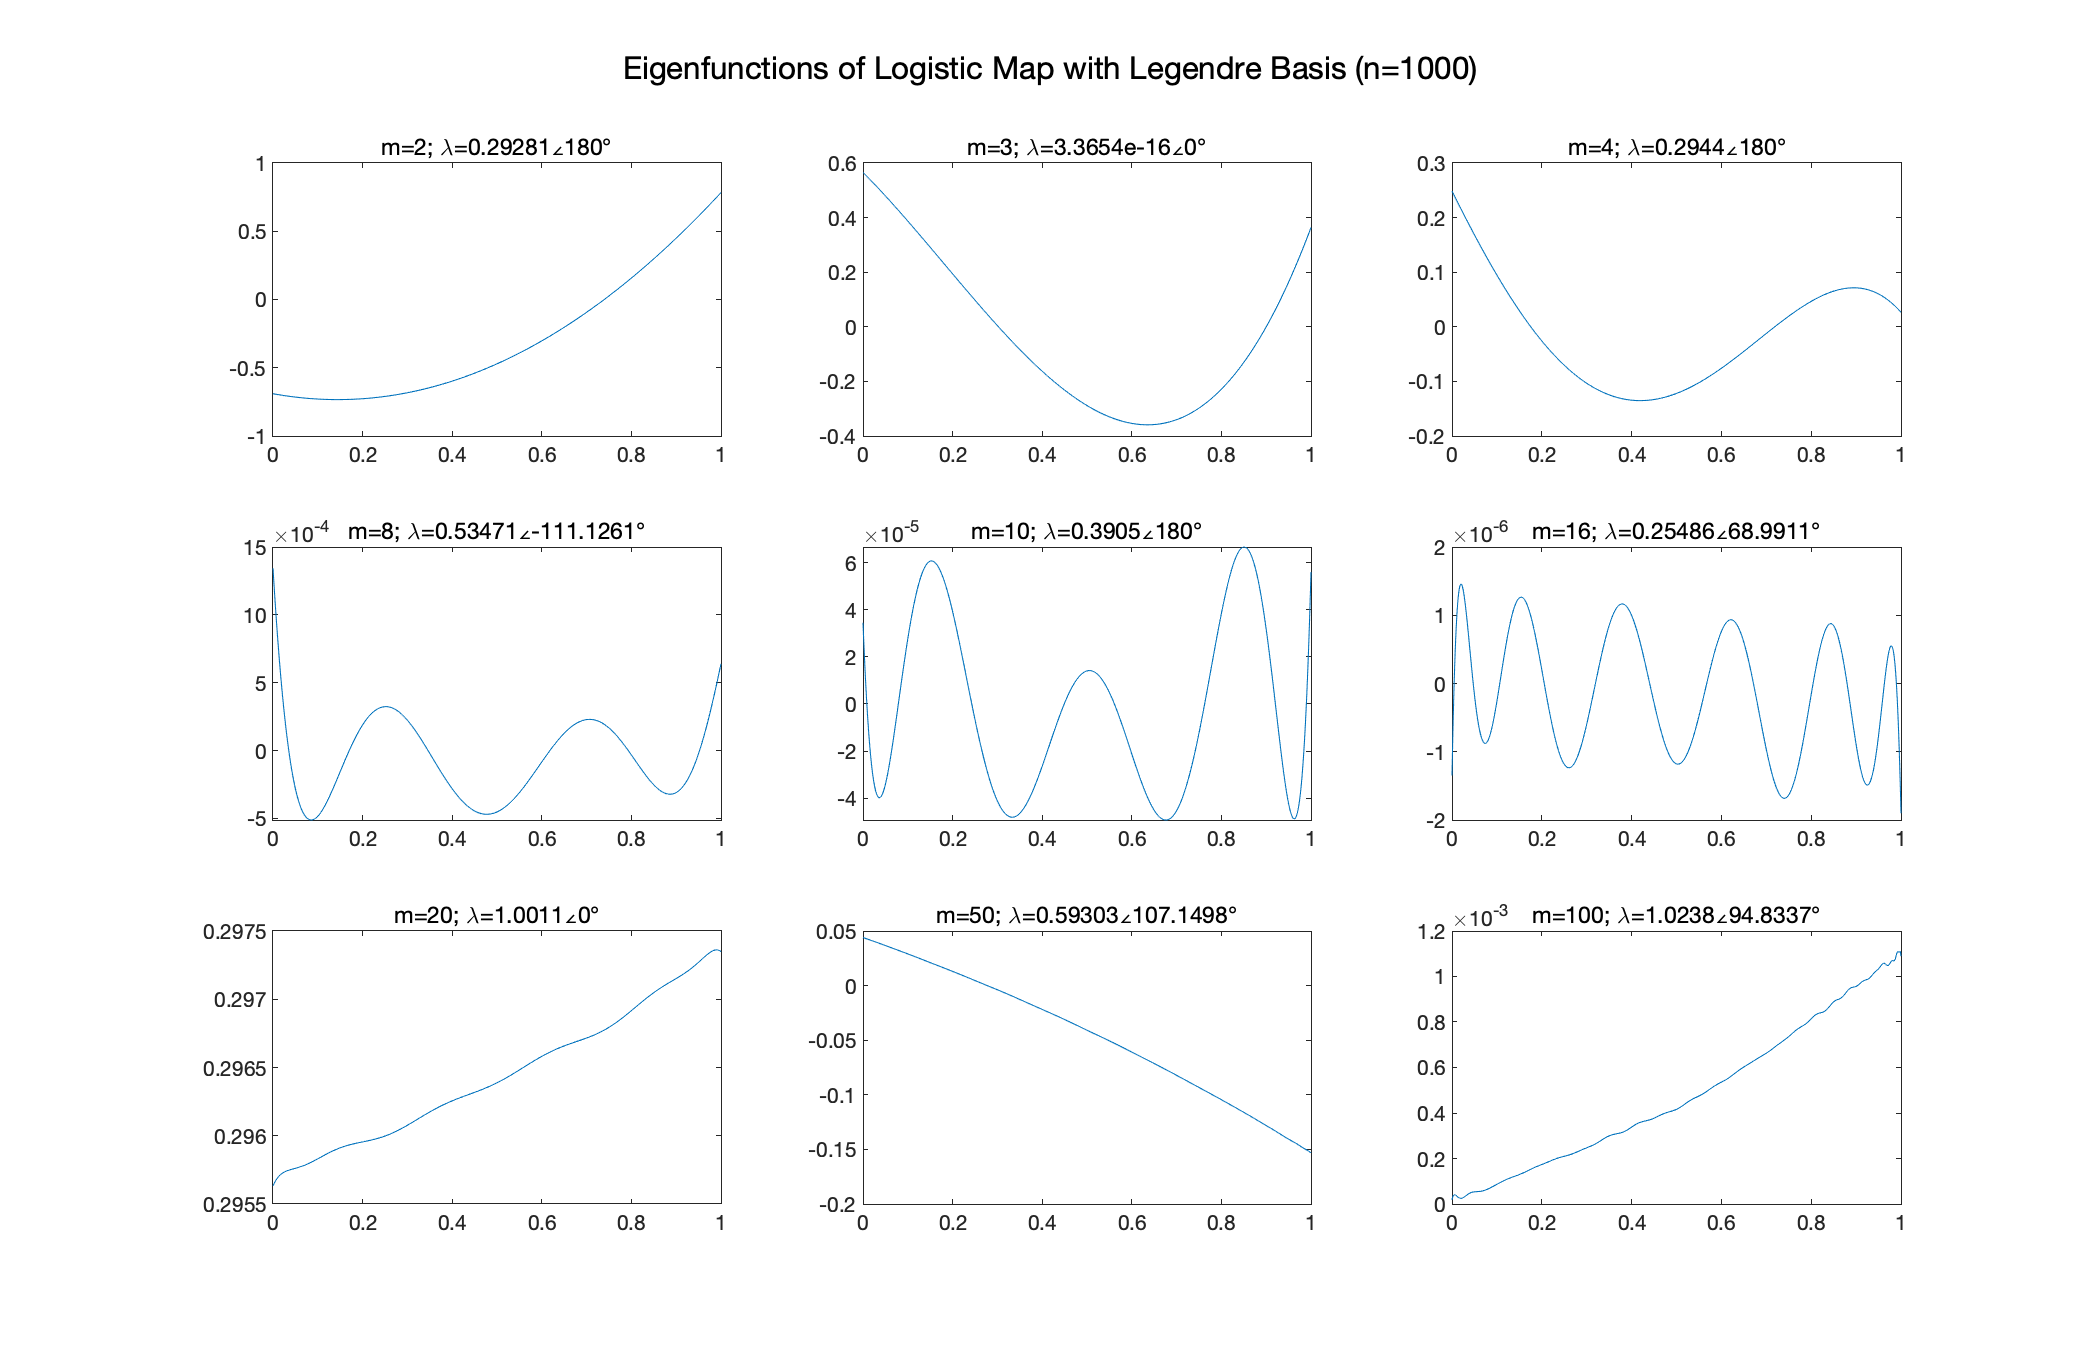
\includegraphics[scale=0.2]{logistic/Logistic_eigen_Legendre_n1000_m2-3-4-8-10-16-20-50-100}}
  \caption{不同基函数数量下Logistic映射的本征函数}
\end{figure}
\subsubsection{自然基函数空间}
\begin{figure}
	\centering
	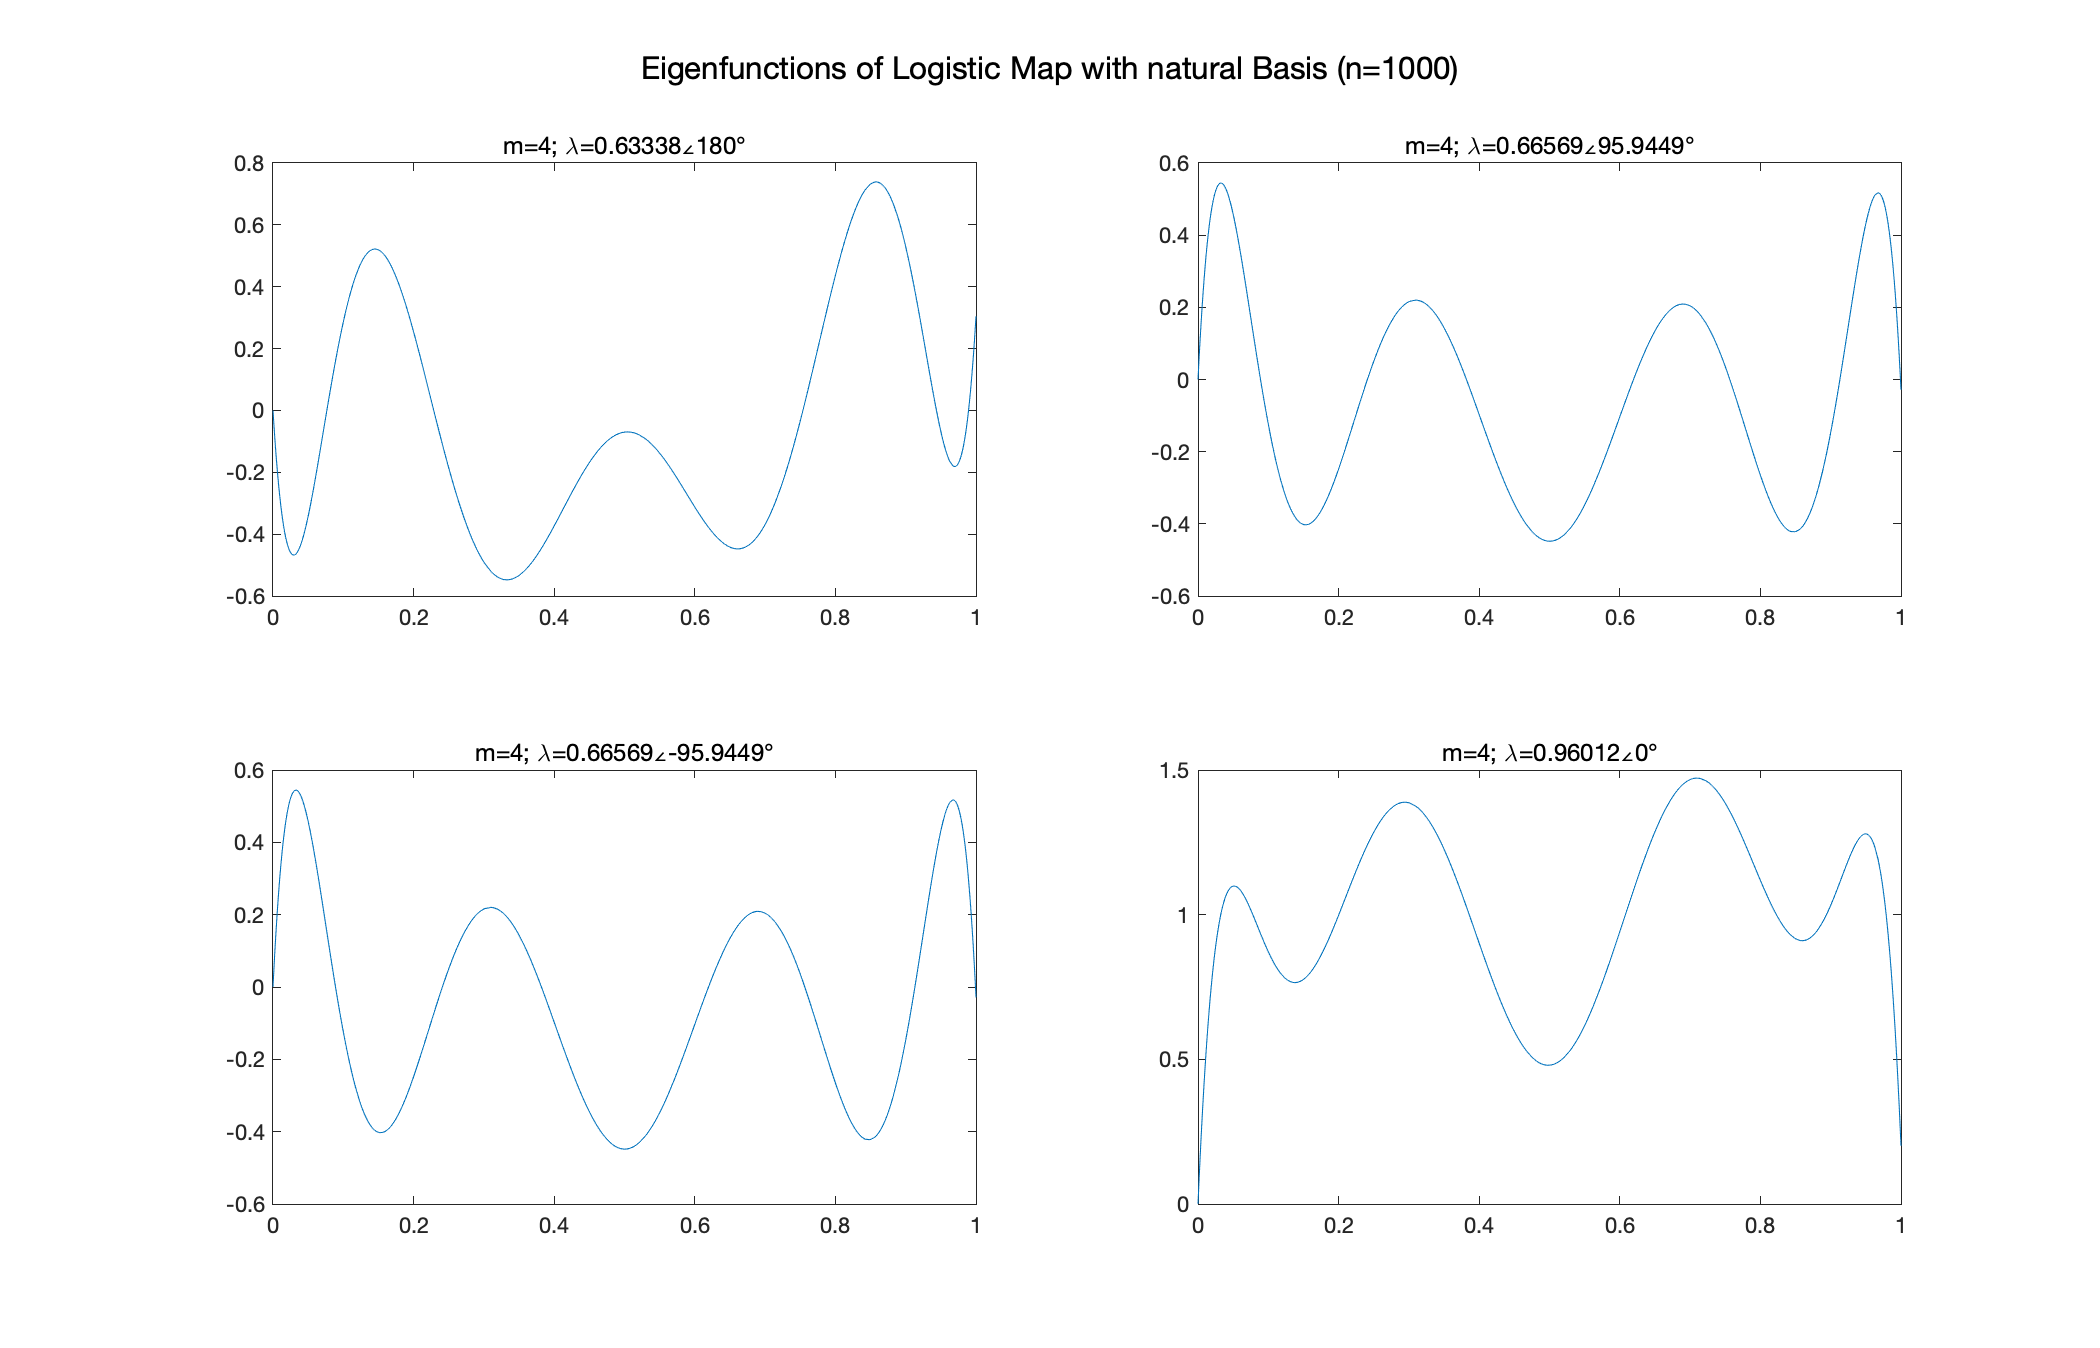
\includegraphics[scale=0.4]{logistic/Logistic_eigen_natural_n1000_m4}
    \caption{自然基函数下Logistic映射的本征函数($m=4$)}
\end{figure}
\begin{figure}
	\centering
	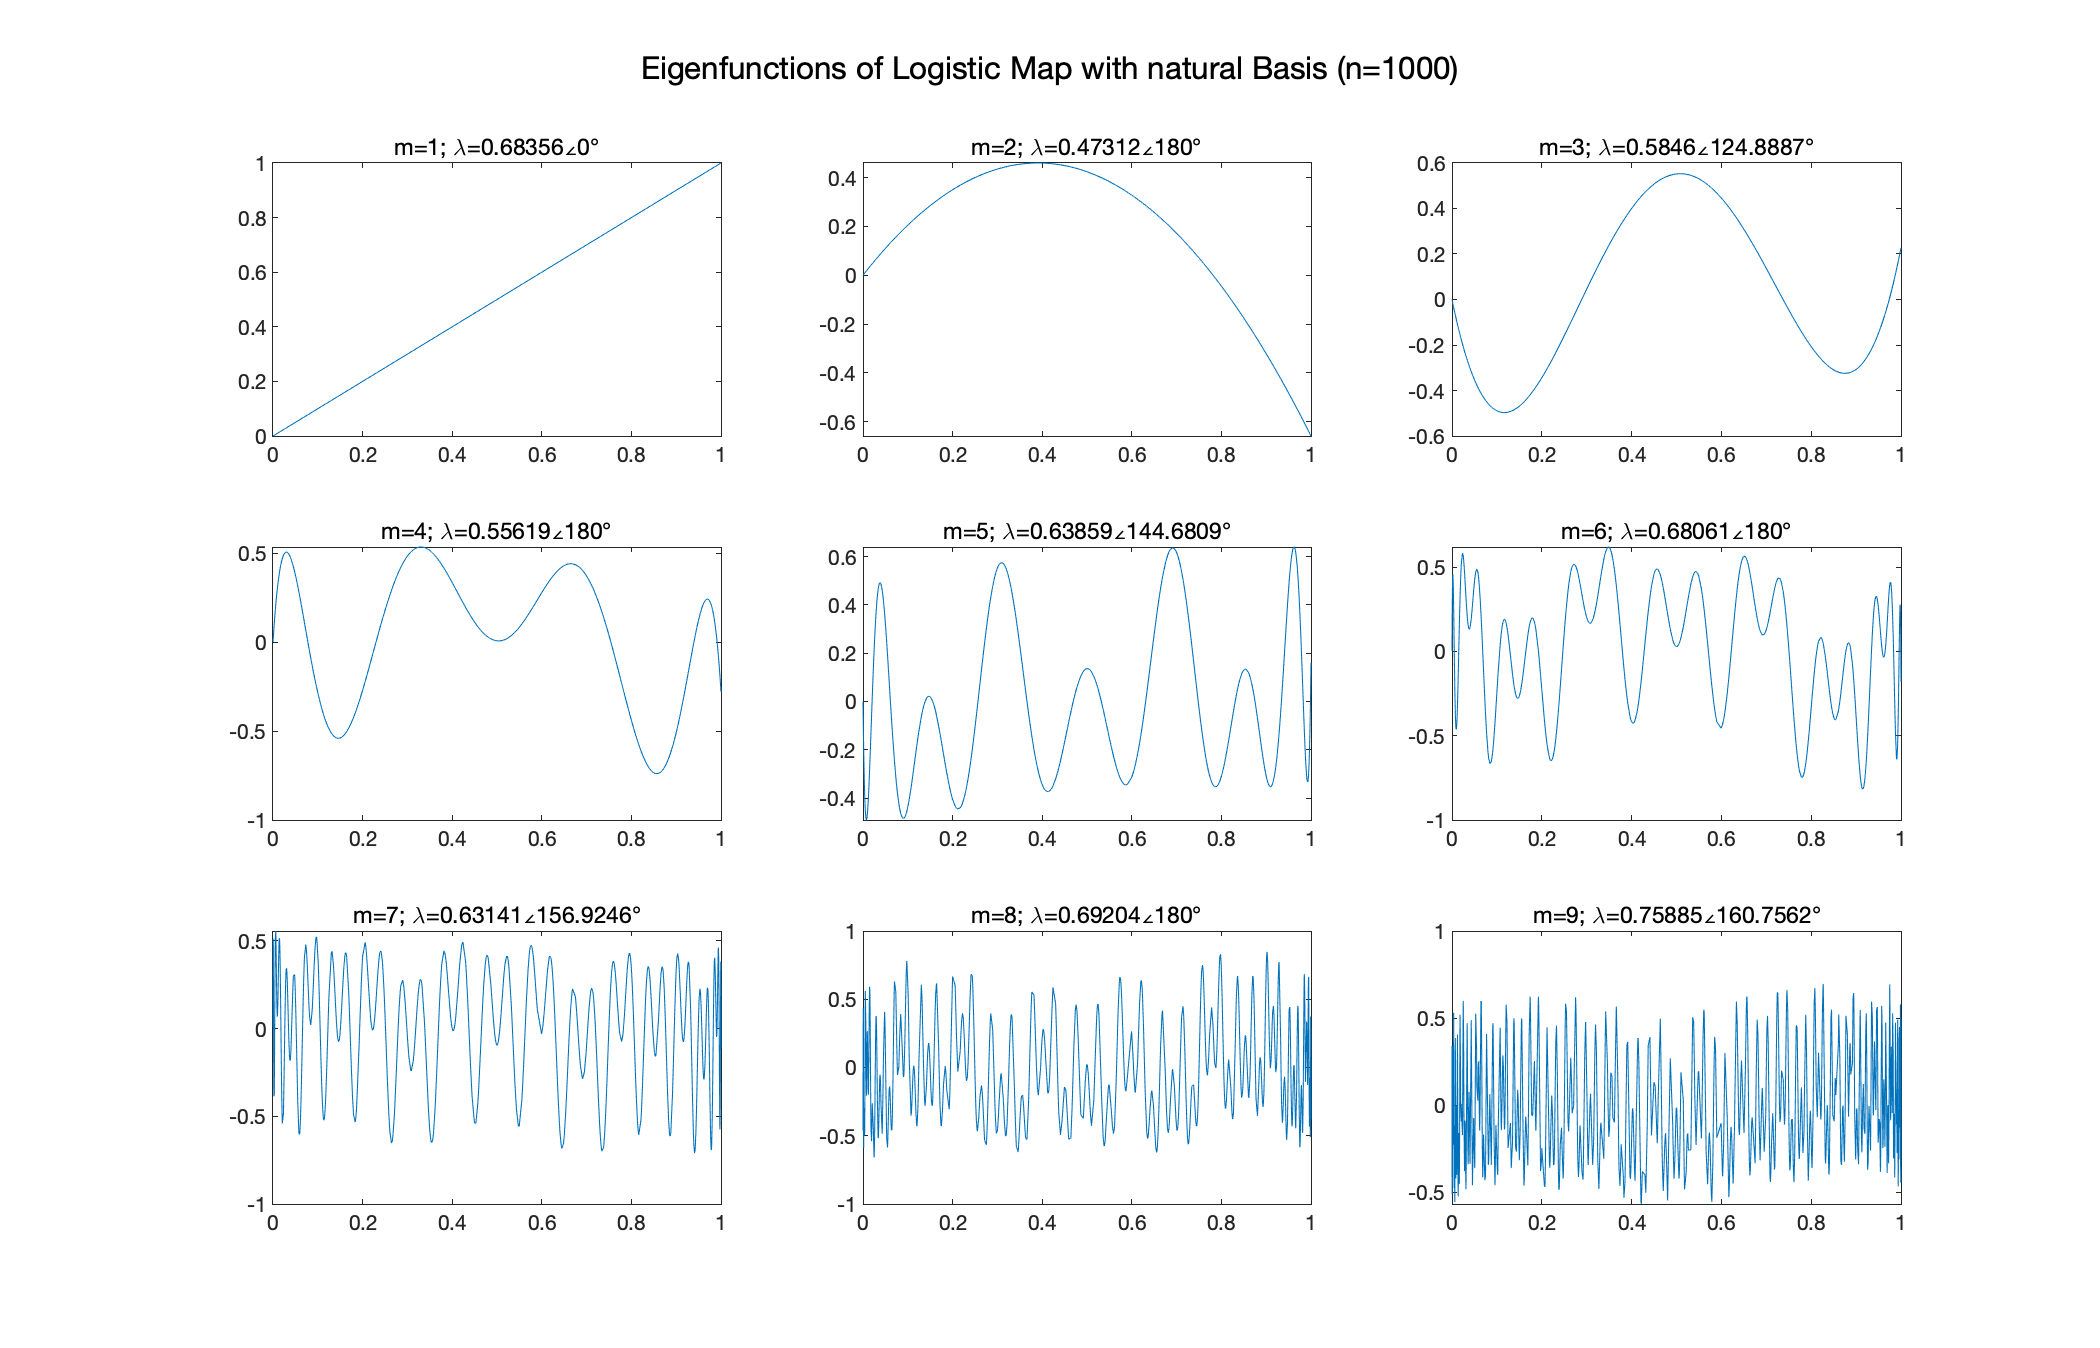
\includegraphics[scale=0.4]{logistic/Logistic_eigen_natural_n1000_m1-2-3-4-5-6-7-8-9}
    \caption{不同基函数数量下Logistic映射的本征函数}
\end{figure}

\subsection{Koopman算符对Logistic映射的相空间划分}
\begin{table}[]
    \centering
    \begin{tabular}{|c|c|}
    \hline
    迭代次数 & 边界点($x=0$) \\ \hline
    1 & 0,\textbf{\underline{1}} \\ \hline
    2 & 0,\textbf{\underline{0.5}},1 \\ \hline
    3 & 0,\textbf{\underline{0.1464}},0.5,\textbf{\underline{0.8536}},1 \\ \hline
    4 & 0,\textbf{\underline{0.0381}},0.1464,\textbf{\underline{0.3087}},0.5,\textbf{\underline{0.6913}},0.8536,\textbf{\underline{0.9619}},1 \\ \hline
    5 & \begin{tabular}[c]{@{}l@{}}0,\textbf{\underline{0.0096}},0.0381,\textbf{\underline{0.0843}},0.1464,\textbf{\underline{0.2222}},0.3087,\textbf{\underline{0.4024}},\\ 0.5,\textbf{\underline{0.5975}},0.6913,\textbf{\underline{0.7778}},0.8536,\textbf{\underline{0.9157}},0.9619,\textbf{\underline{0.9904}},1\end{tabular} \\ \hline
    \end{tabular}
    \caption{Logistic映射的边界点($x=0$)}
\end{table}

\begin{figure}
	\centering
	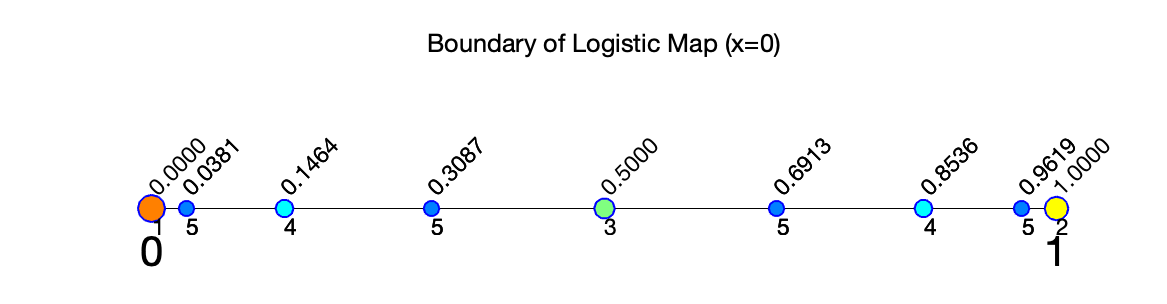
\includegraphics[scale=0.8]{logistic/Logistic_boundarys_x0}
    \caption{Logistic映射的边界点($x=0$)}
\end{figure}

\begin{table}[]
    \centering
    \begin{tabular}{|c|c|}
    \hline
    迭代次数 & 边界点($x=\frac{3}{4}$) \\ \hline
    0 & 0.75 \\ \hline
    1 & \textbf{\underline{0.25}},0.75 \\ \hline
    2 & \textbf{\underline{0.0670}},0.25,0.75,\textbf{\underline{0.9330}} \\ \hline
    3 & \textbf{\underline{0.0170}},0.0670,0.25,\textbf{\underline{0.3706}},\textbf{\underline{0.6294}},0.75,0.9330,\textbf{\underline{0.9830}} \\ \hline
    4 & \begin{tabular}[c]{@{}l@{}}\textbf{\underline{0.0043}},0.0170,0.0670,\textbf{\underline{0.1033}},\textbf{\underline{0.1956}},0.25,0.3706,\textbf{\underline{0.4347}},\\ \textbf{\underline{0.5653}},0.6294,0.75,\textbf{\underline{0.8044}},\textbf{\underline{0.8967}},0.9330,0.9830,\textbf{\underline{0.9957}}\end{tabular} \\ \hline
    \end{tabular}
    \caption{Logistic映射的边界点($x=\frac{3}{4}$)}
\end{table}

\begin{figure}
	\centering
	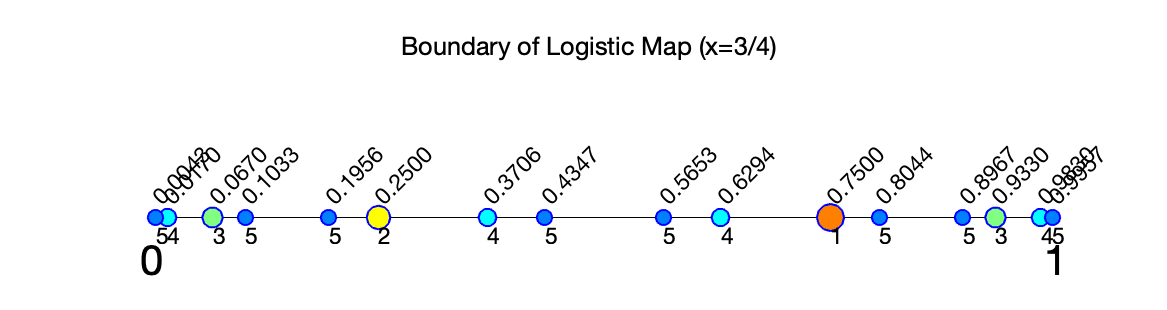
\includegraphics[scale=0.8]{logistic/Logistic_boundarys_x3-4}
    \caption{Logistic映射的边界点($x=\frac{3}{4}$)}
\end{figure}

\begin{figure}
    \centering%[2,3,4,5,8,10,15,20]
    \subfloat[m=2]{
      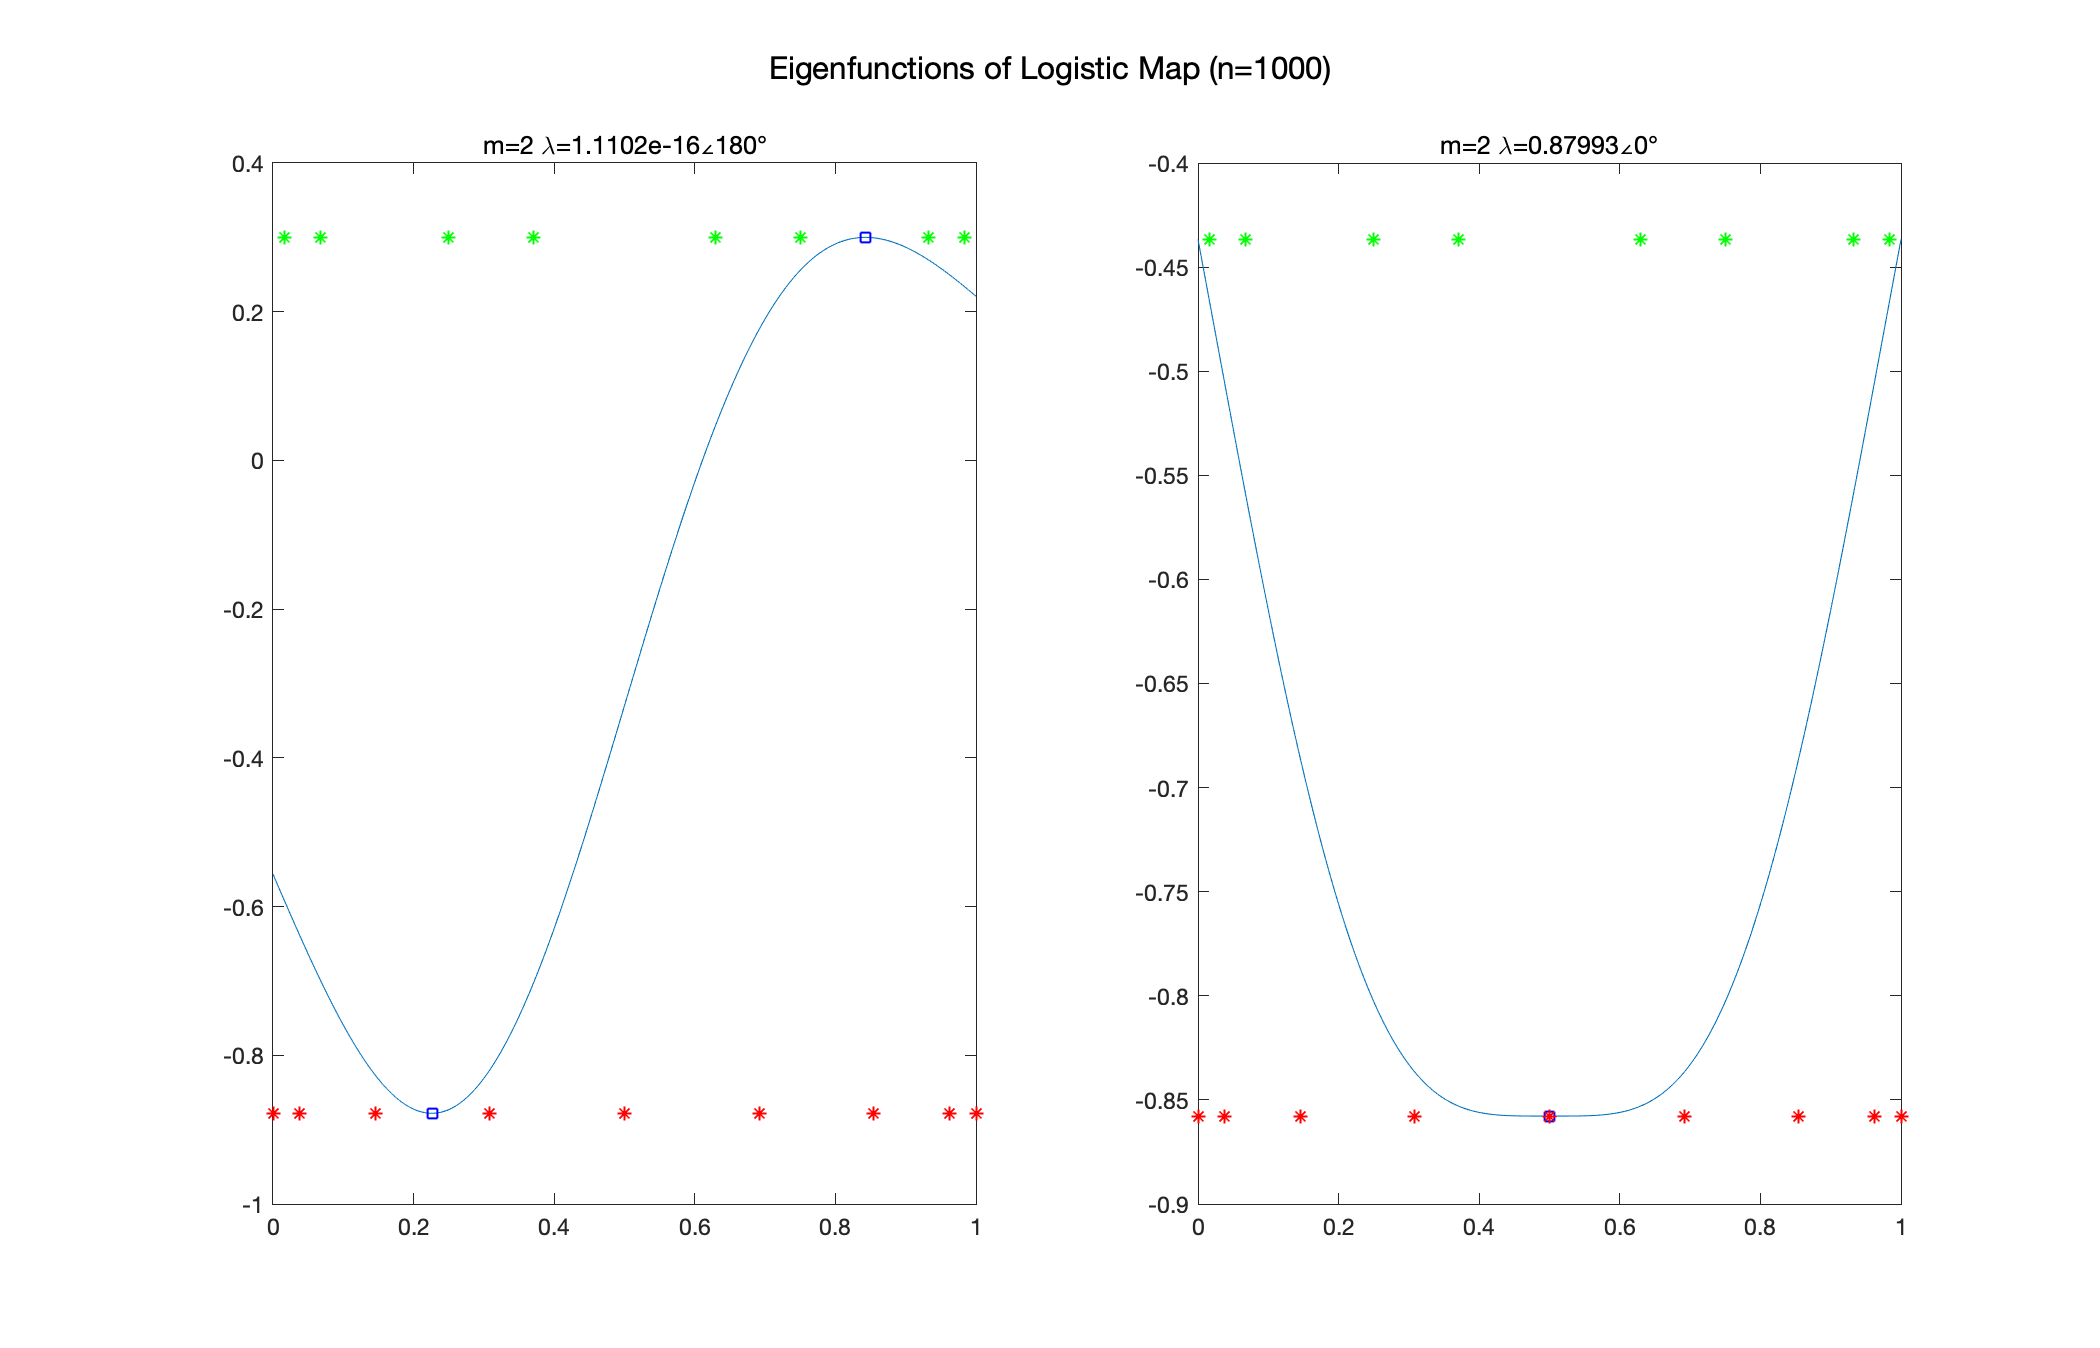
\includegraphics[scale=0.2]{logistic/noise/Logistic_eigen_noise_n1000m2d0}}
    \subfloat[m=3]{
      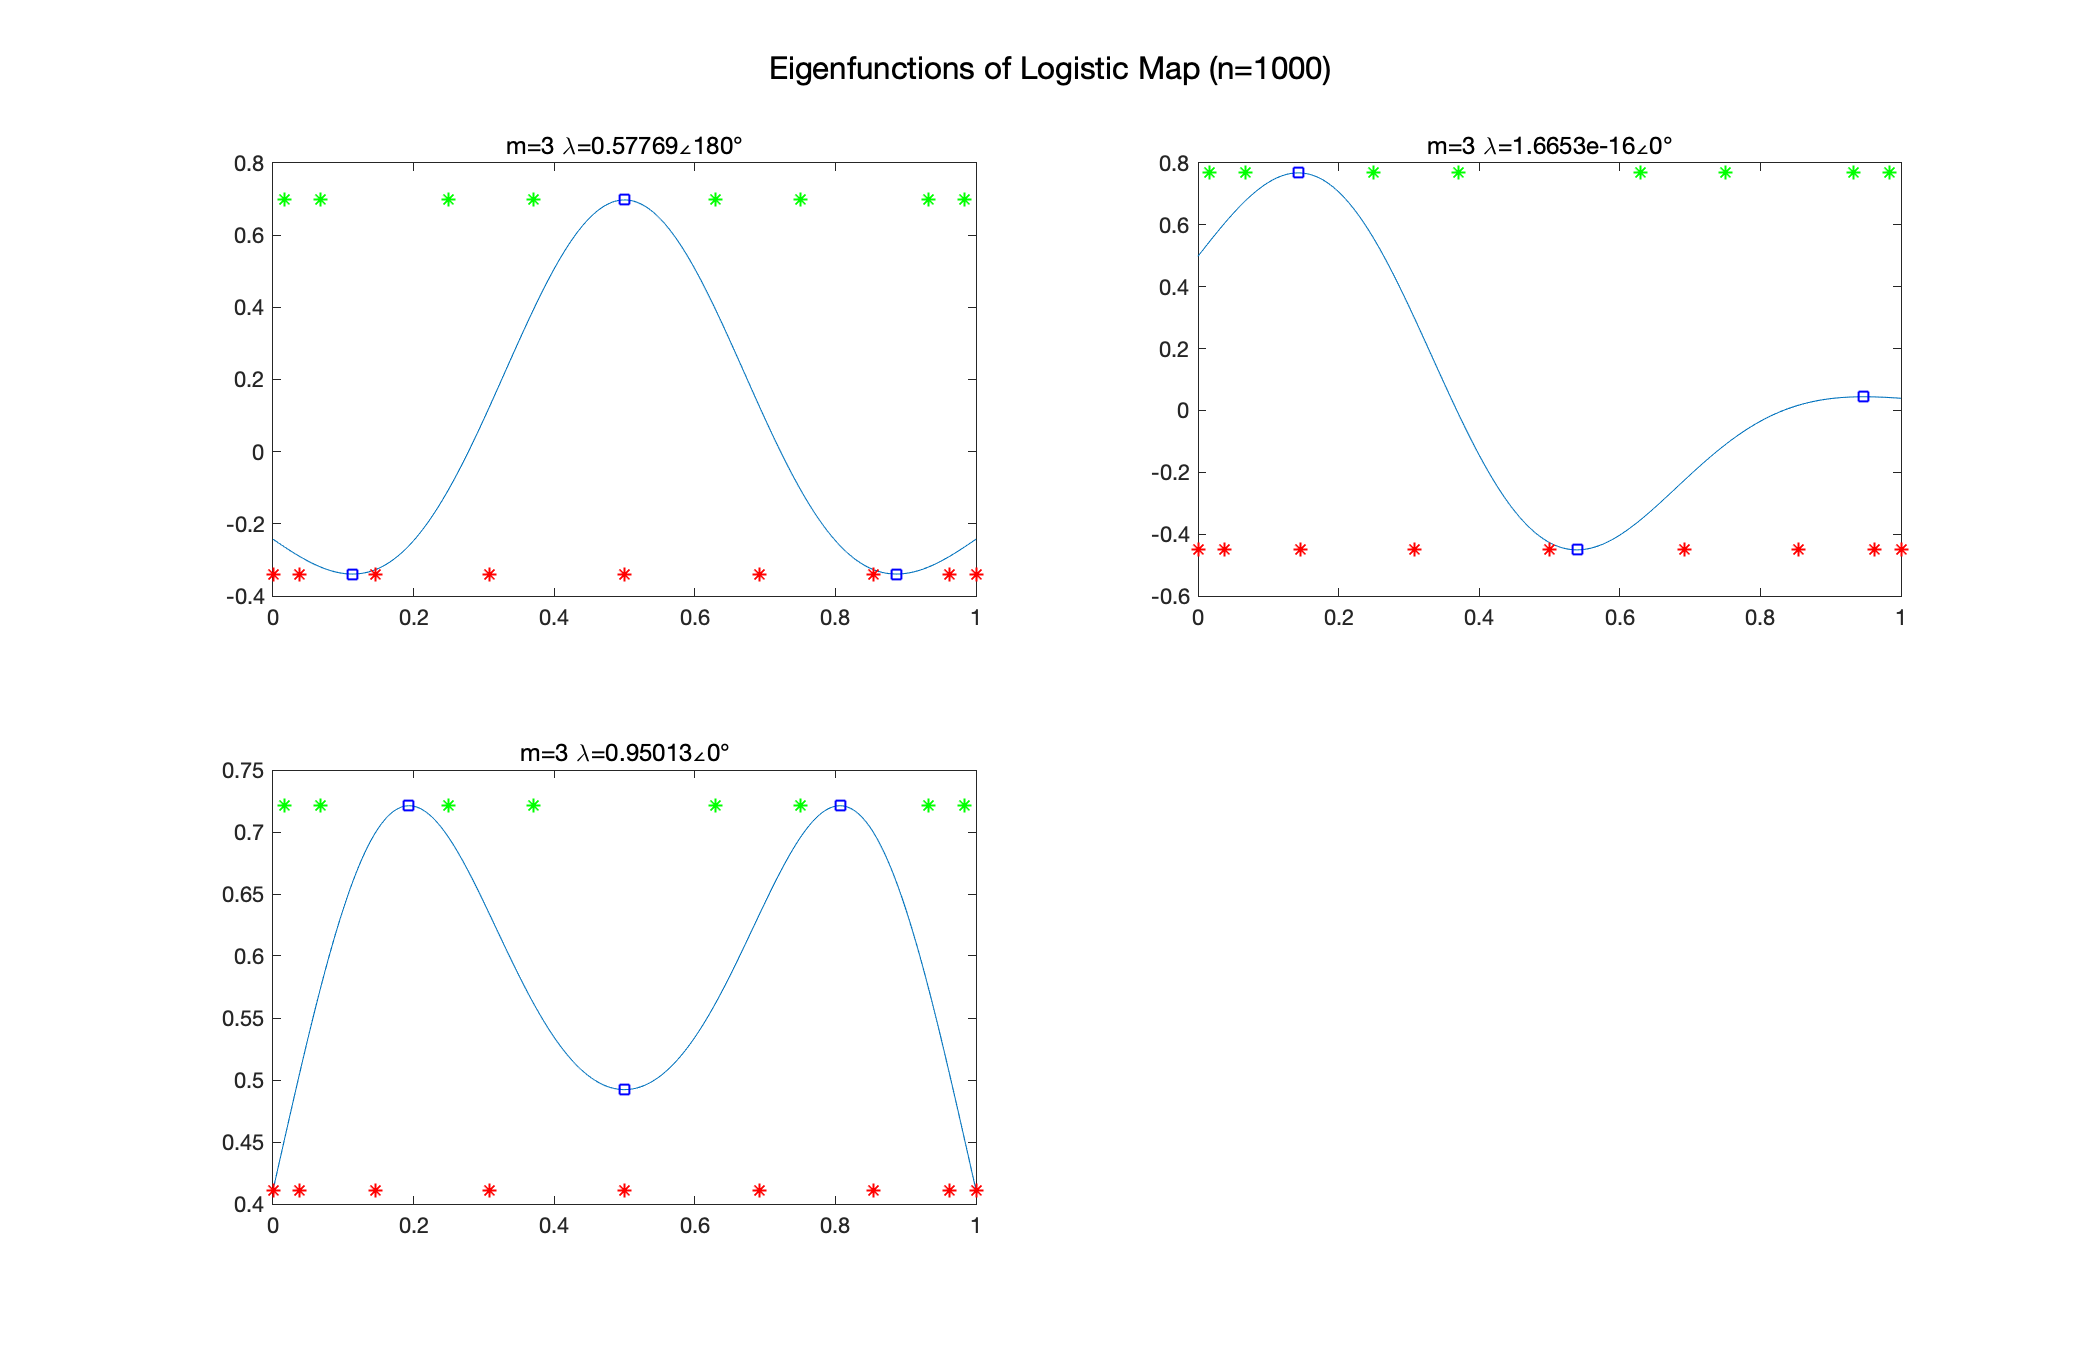
\includegraphics[scale=0.2]{logistic/noise/Logistic_eigen_noise_n1000m3d0}}
      \\
    \subfloat[m=4]{
      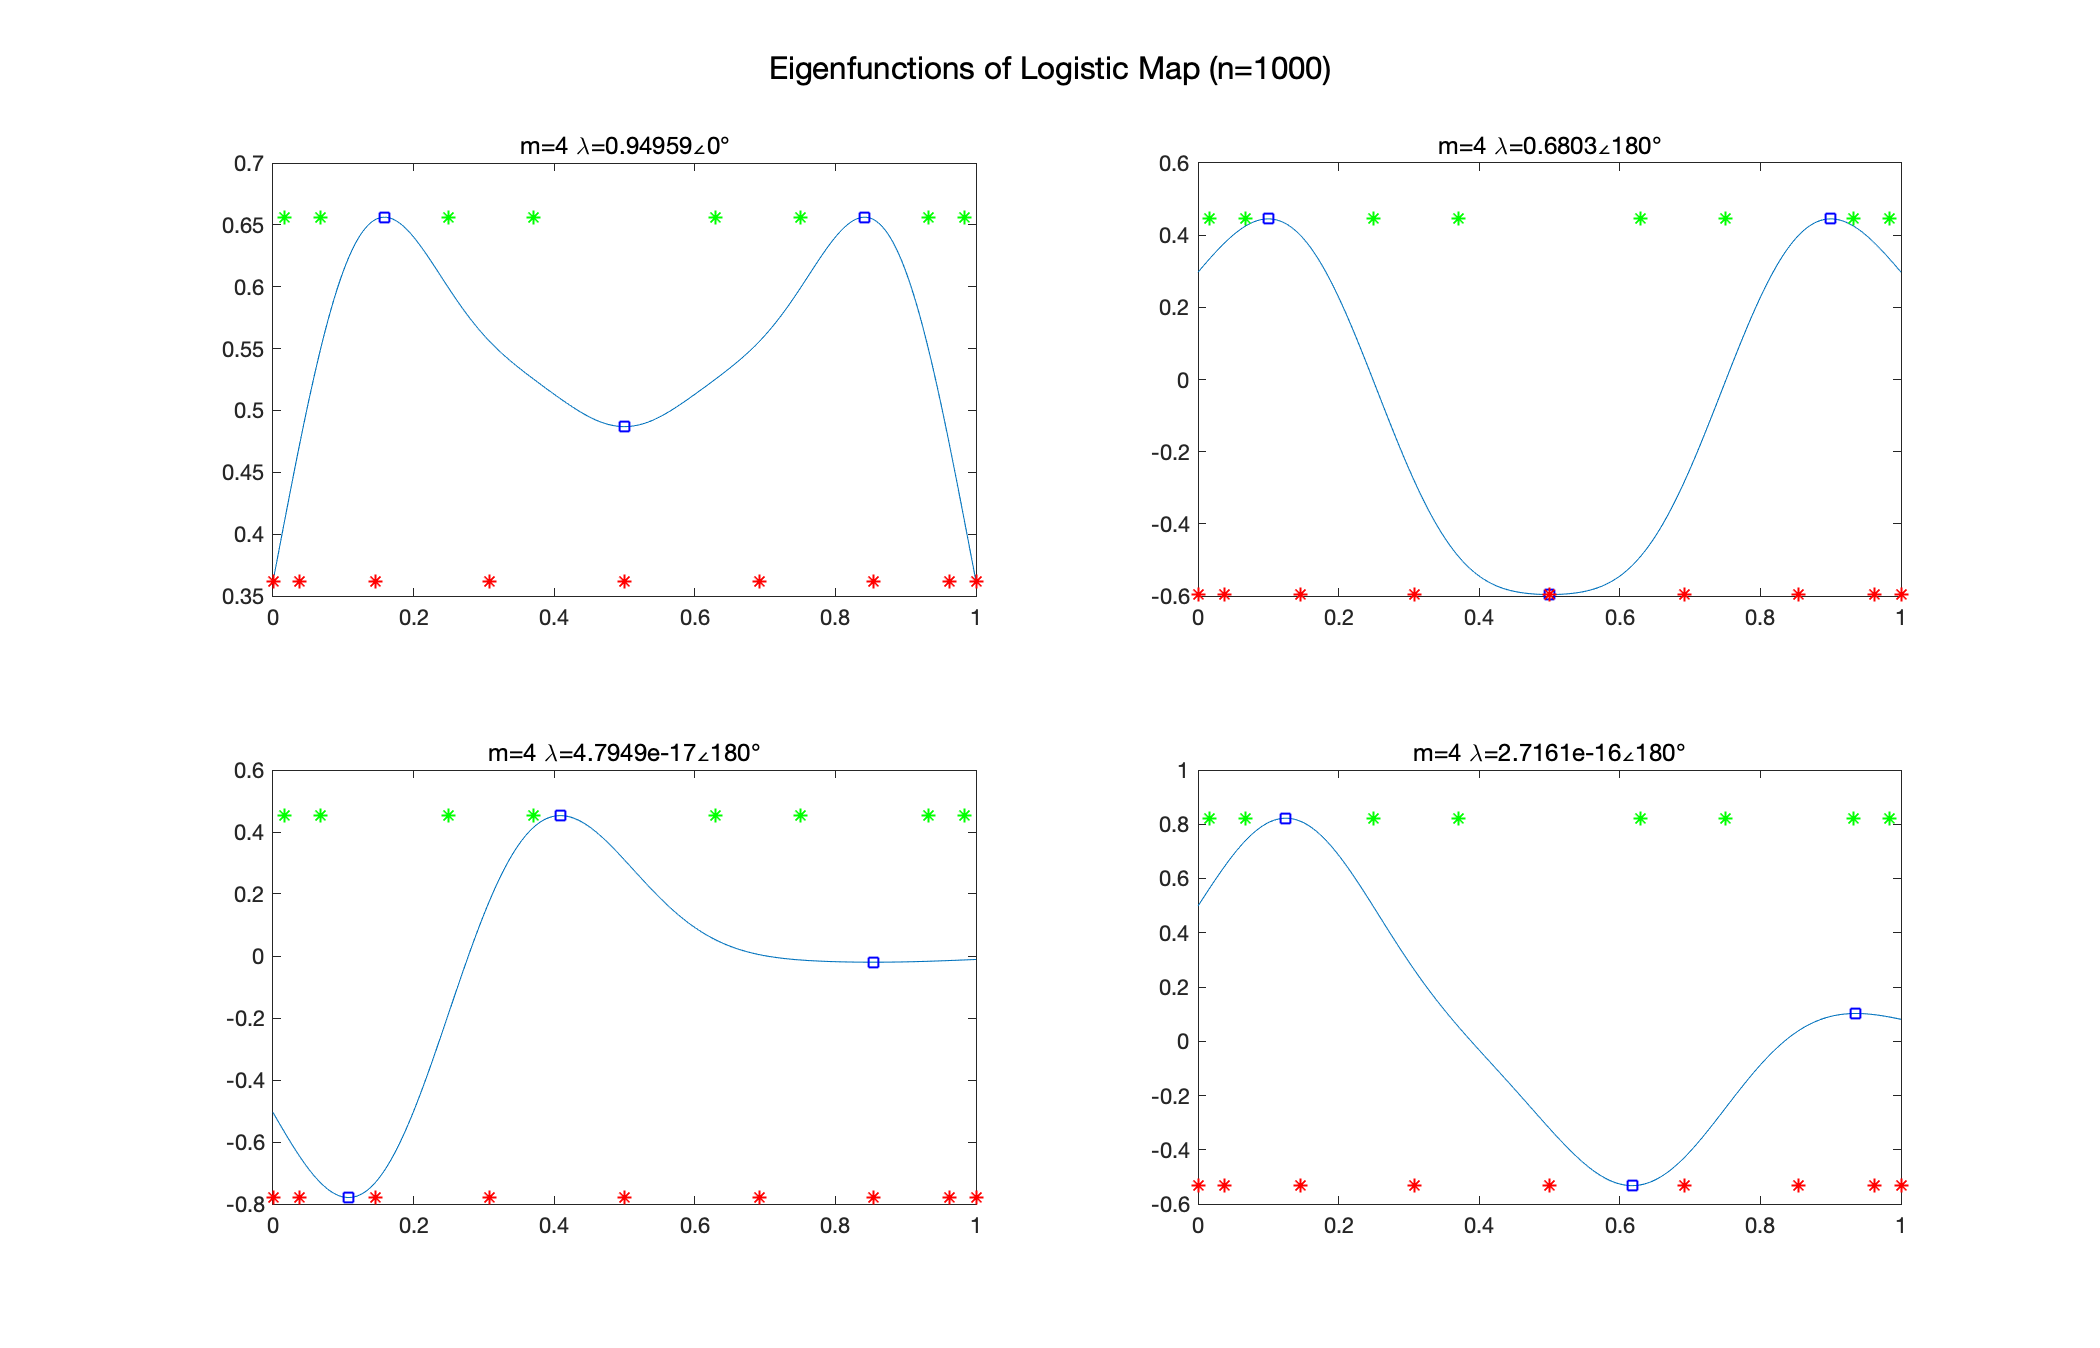
\includegraphics[scale=0.2]{logistic/noise/Logistic_eigen_noise_n1000m4d0}}
    \subfloat[m=5]{
      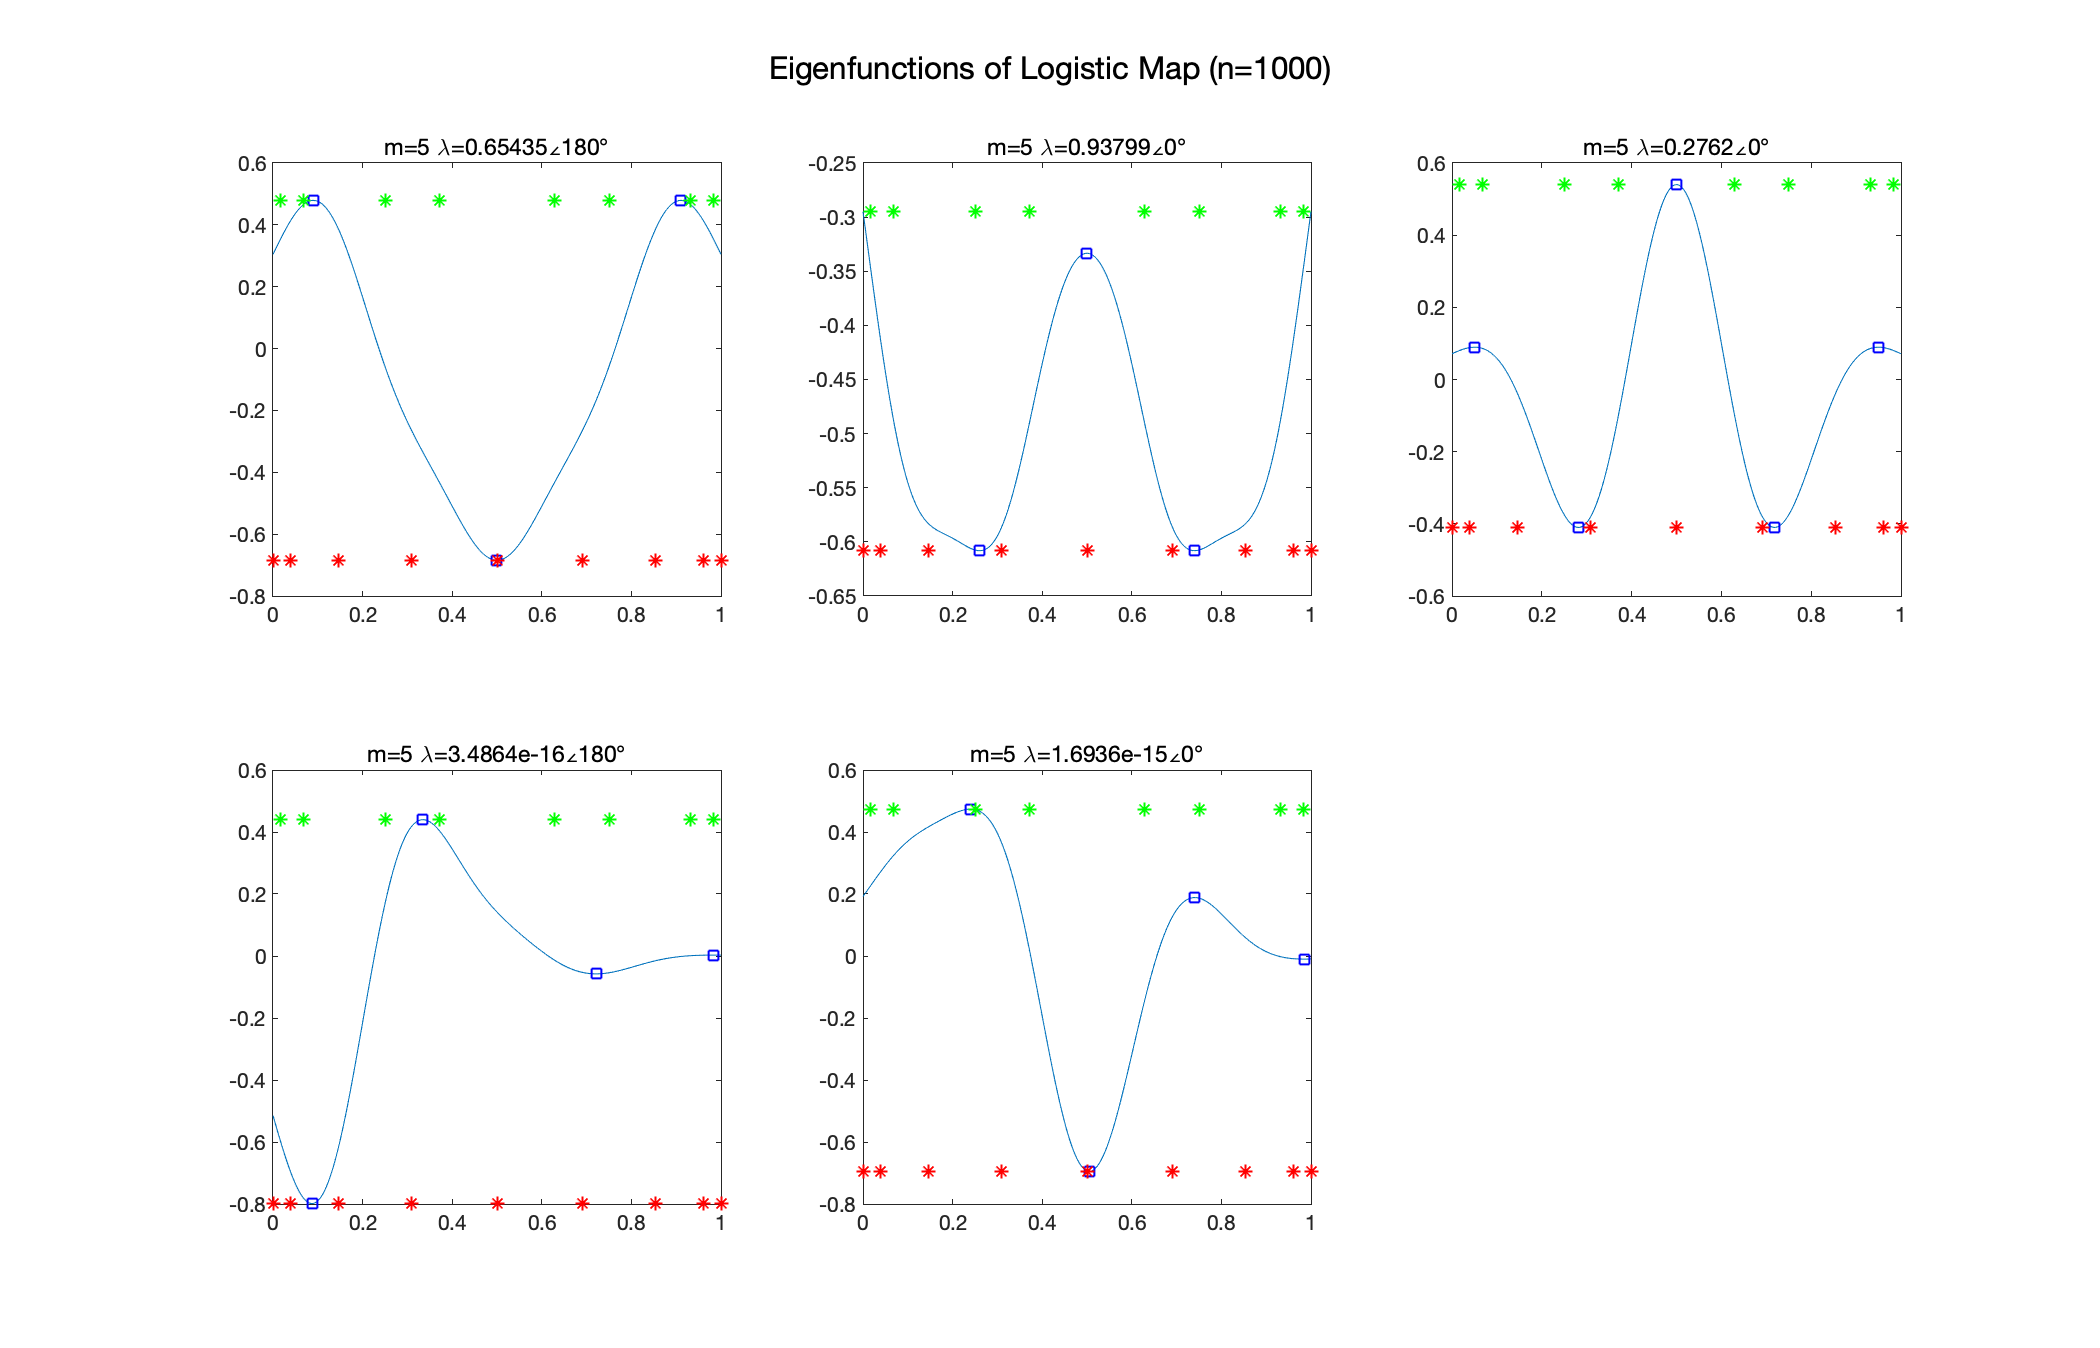
\includegraphics[scale=0.2]{logistic/noise/Logistic_eigen_noise_n1000m5d0}}
      \\
    \subfloat[m=8]{
      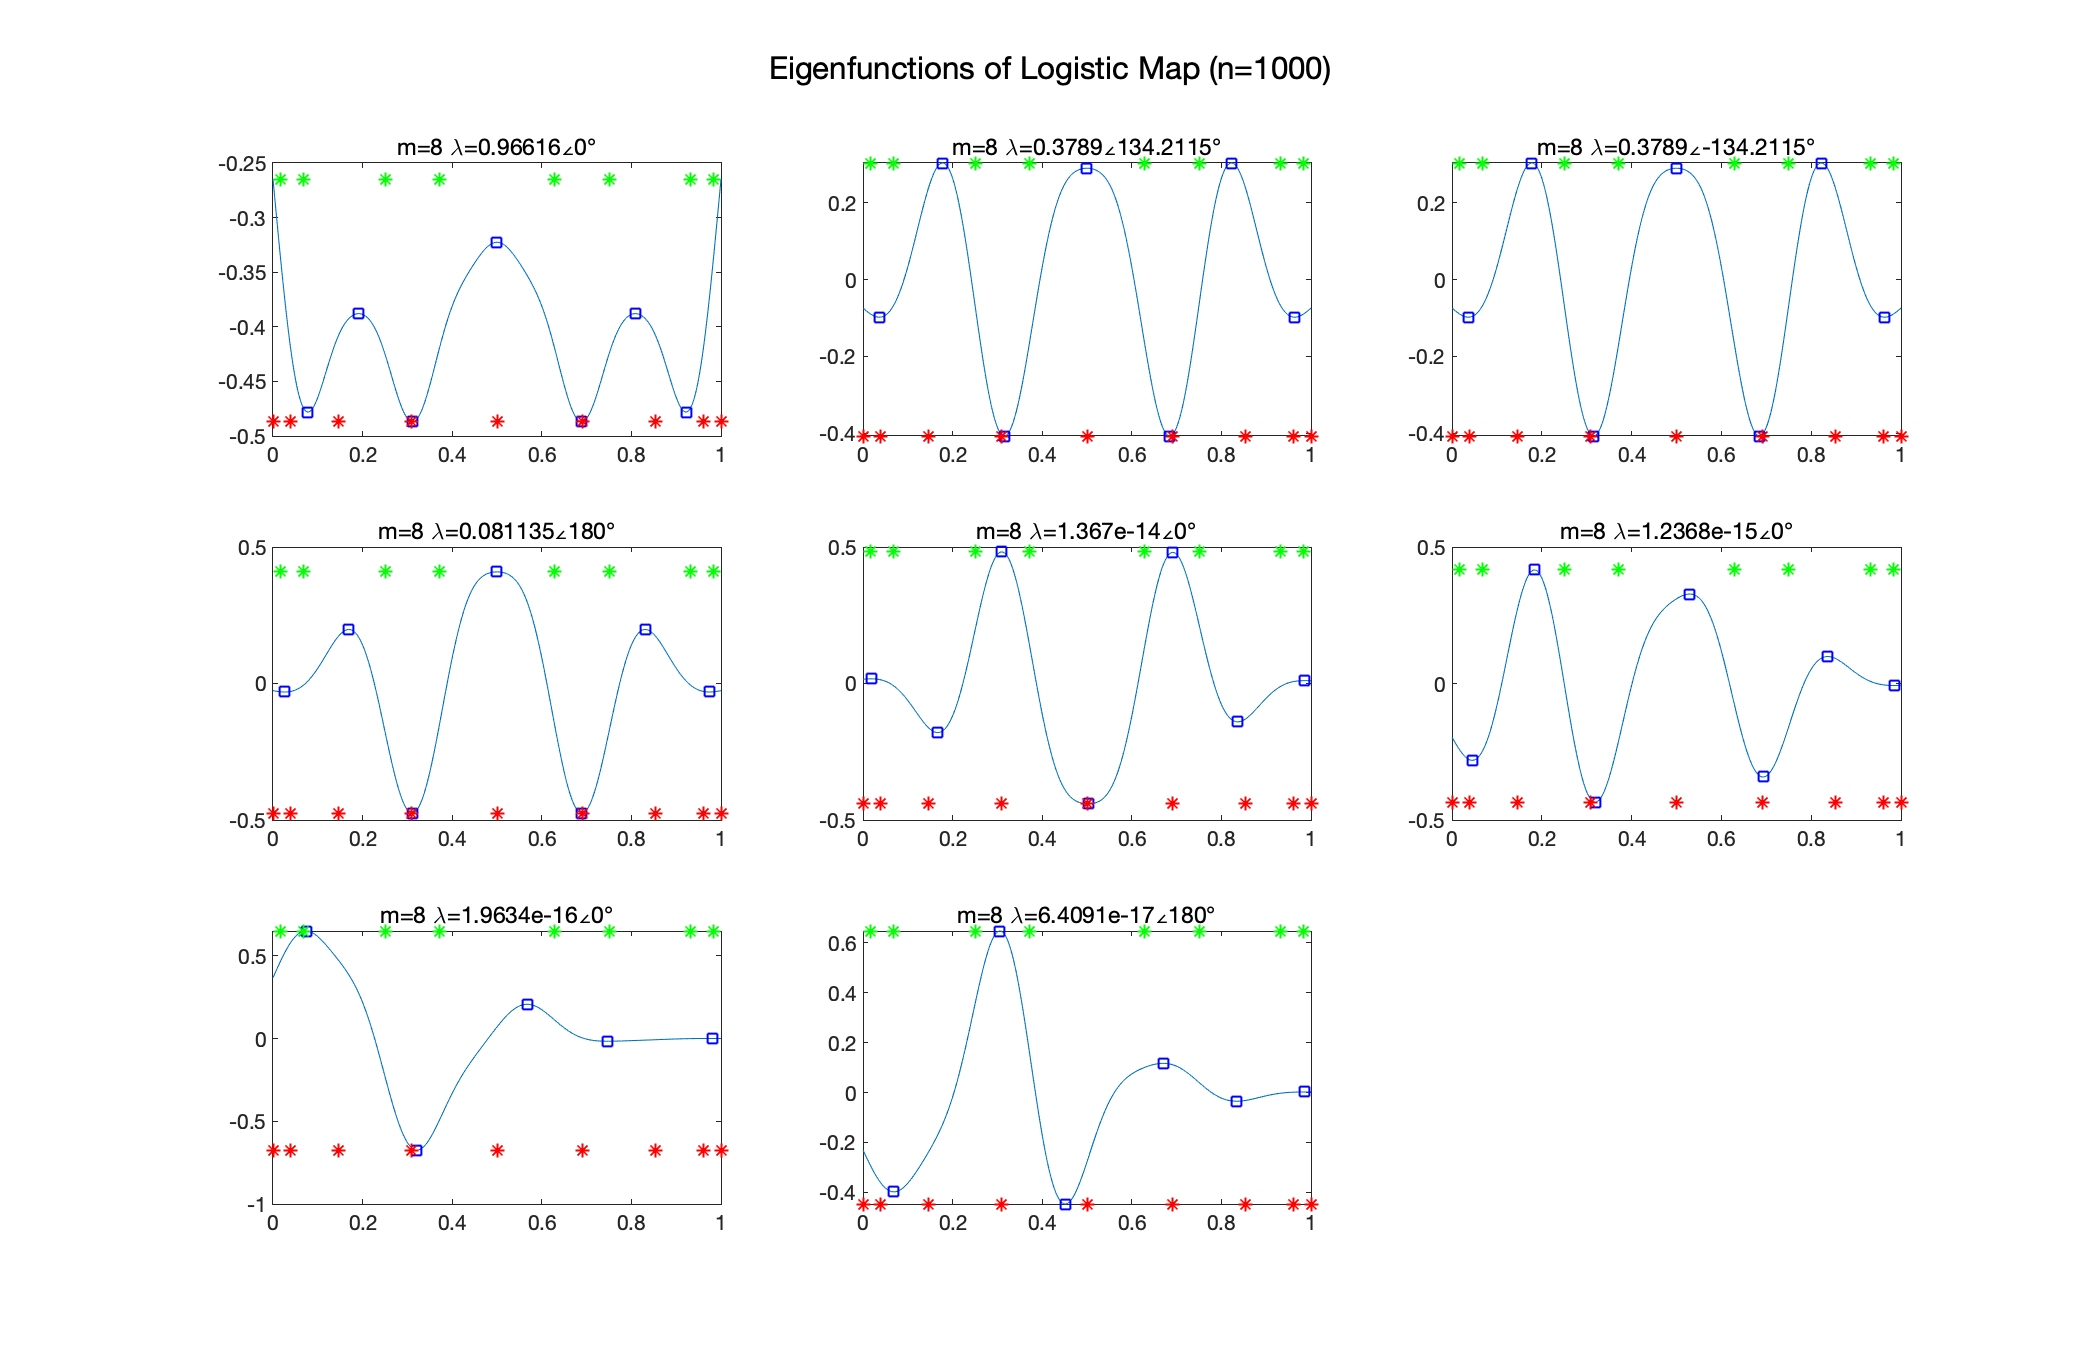
\includegraphics[scale=0.2]{logistic/noise/Logistic_eigen_noise_n1000m8d0}}
    \subfloat[m=10]{
      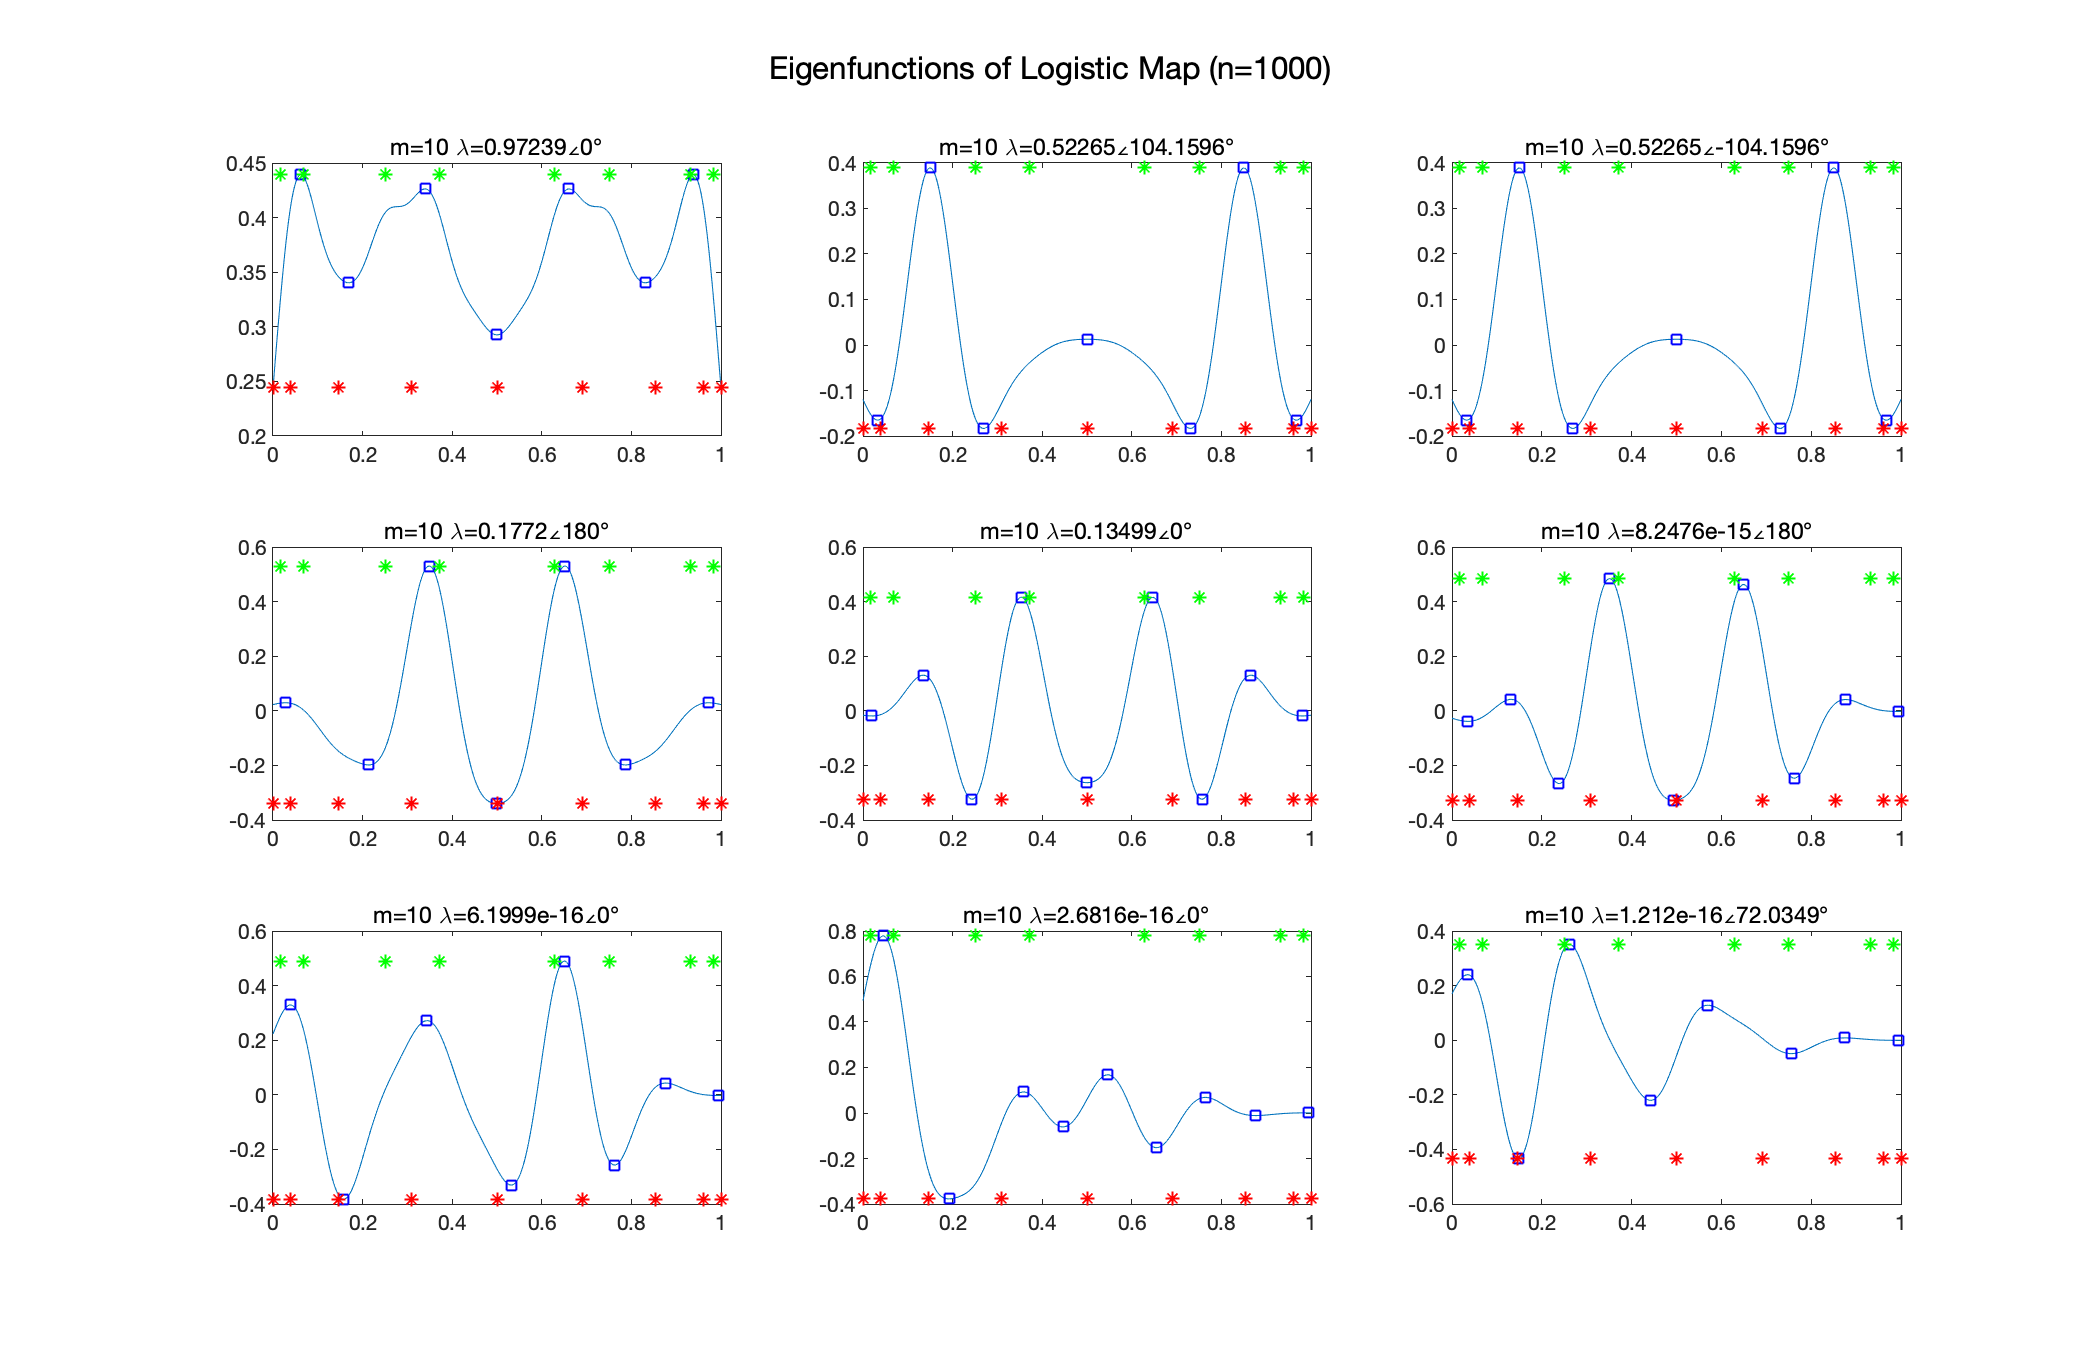
\includegraphics[scale=0.2]{logistic/noise/Logistic_eigen_noise_n1000m10d0}}
      \\
    \subfloat[m=15]{
      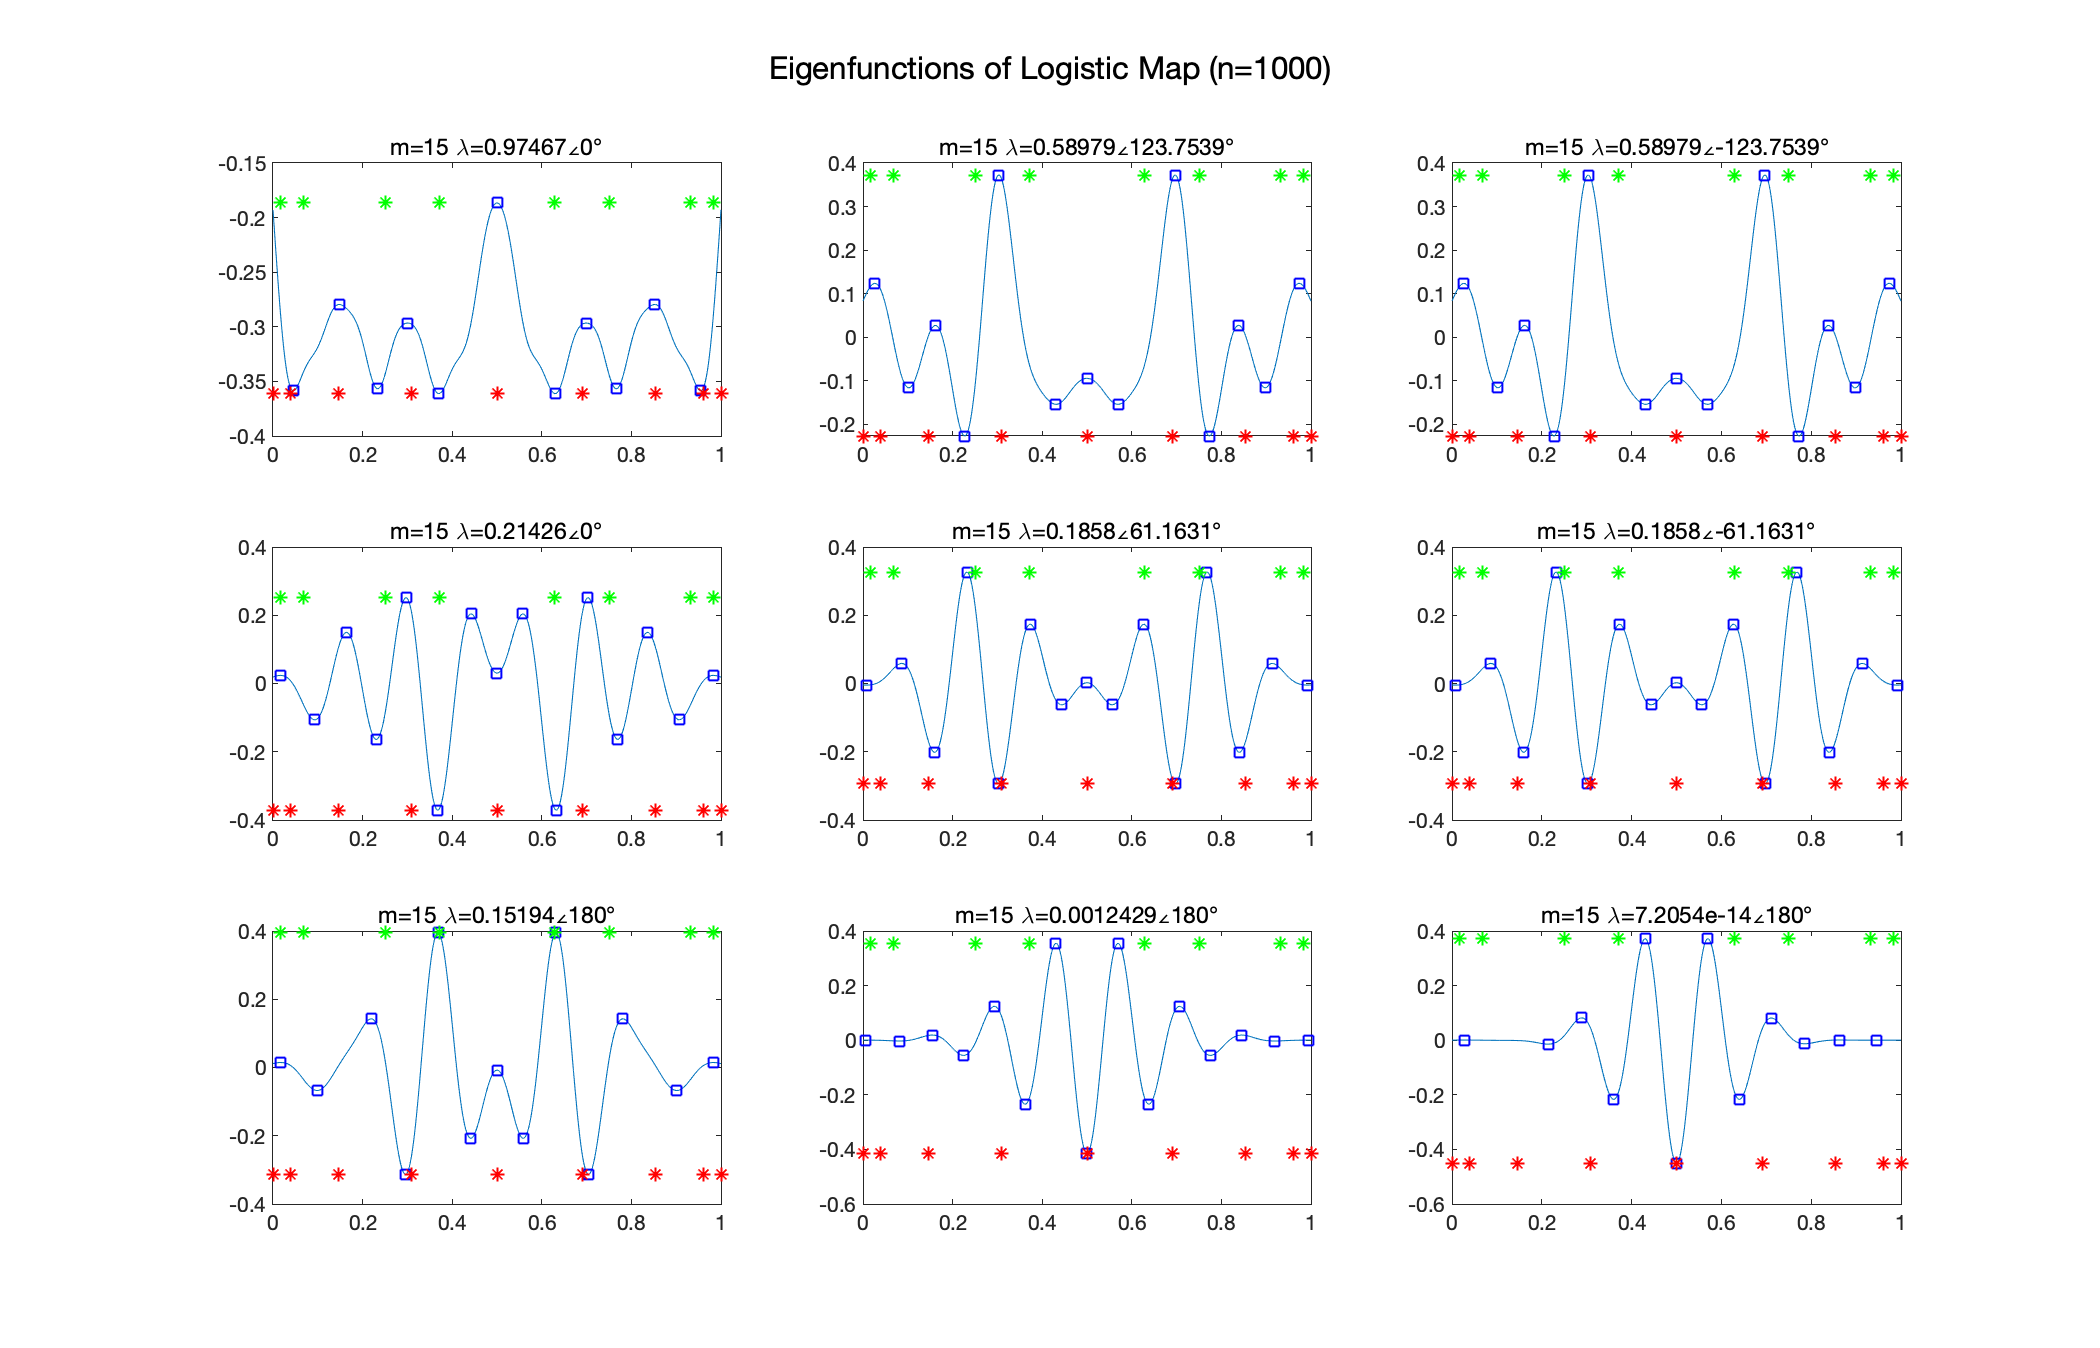
\includegraphics[scale=0.2]{logistic/noise/Logistic_eigen_noise_n1000m15d0}}
    \subfloat[m=20]{
      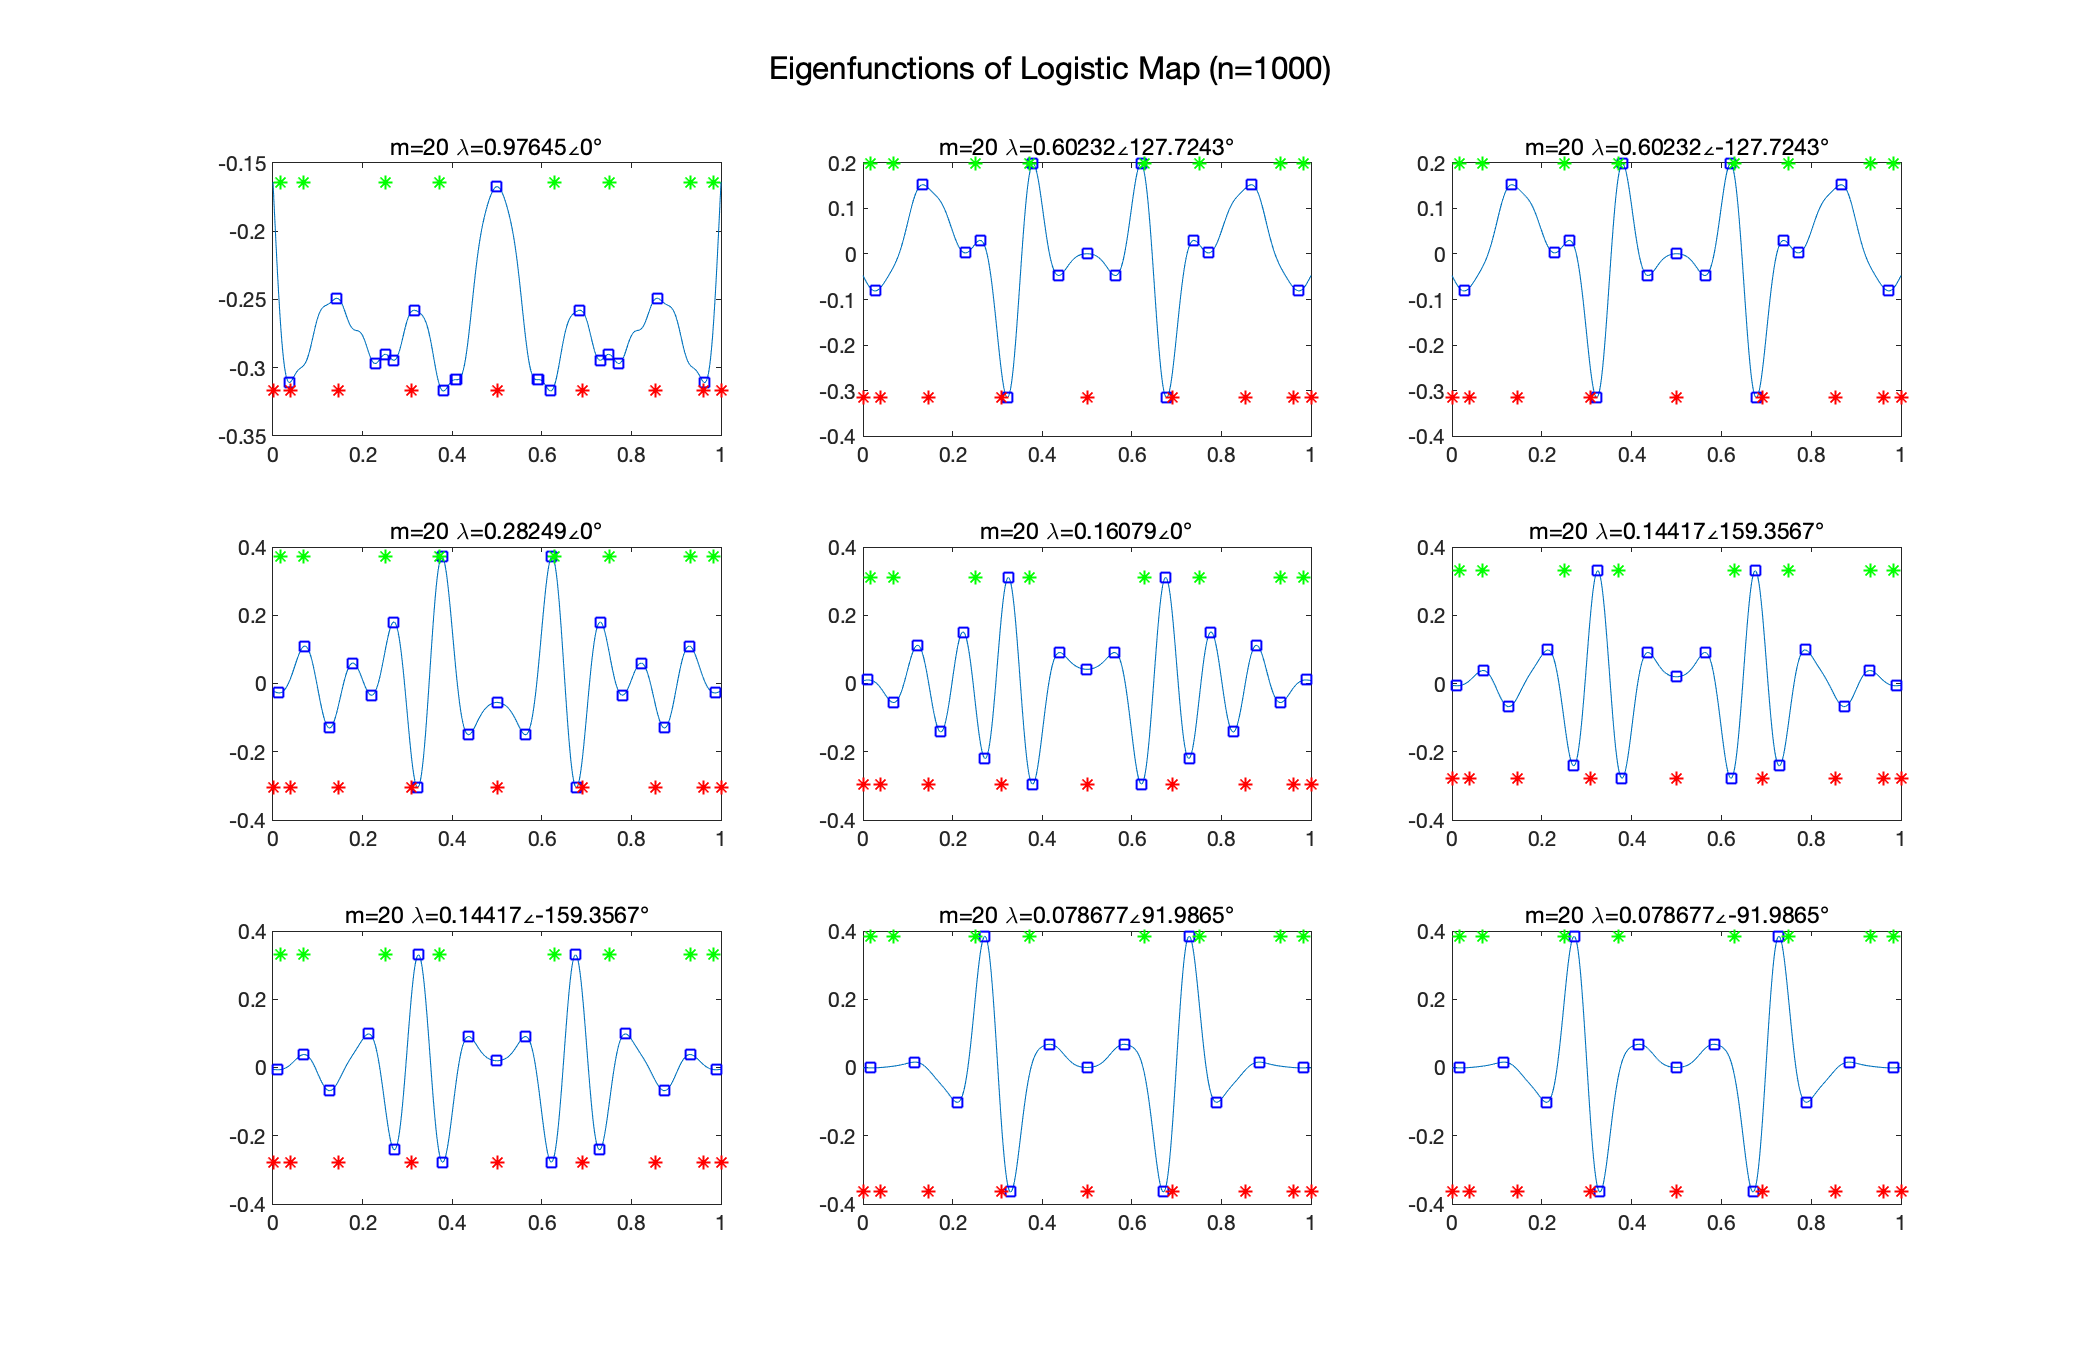
\includegraphics[scale=0.2]{logistic/noise/Logistic_eigen_noise_n1000m20d0}}
      \\
    \caption{Logistic映射的边界点与本征函数}
  \end{figure}

\subsection{更多的讨论}
\subsubsection{噪声对Koopman算符的影响}


\begin{figure}
    \centering
    \subfloat[noise=0]{
      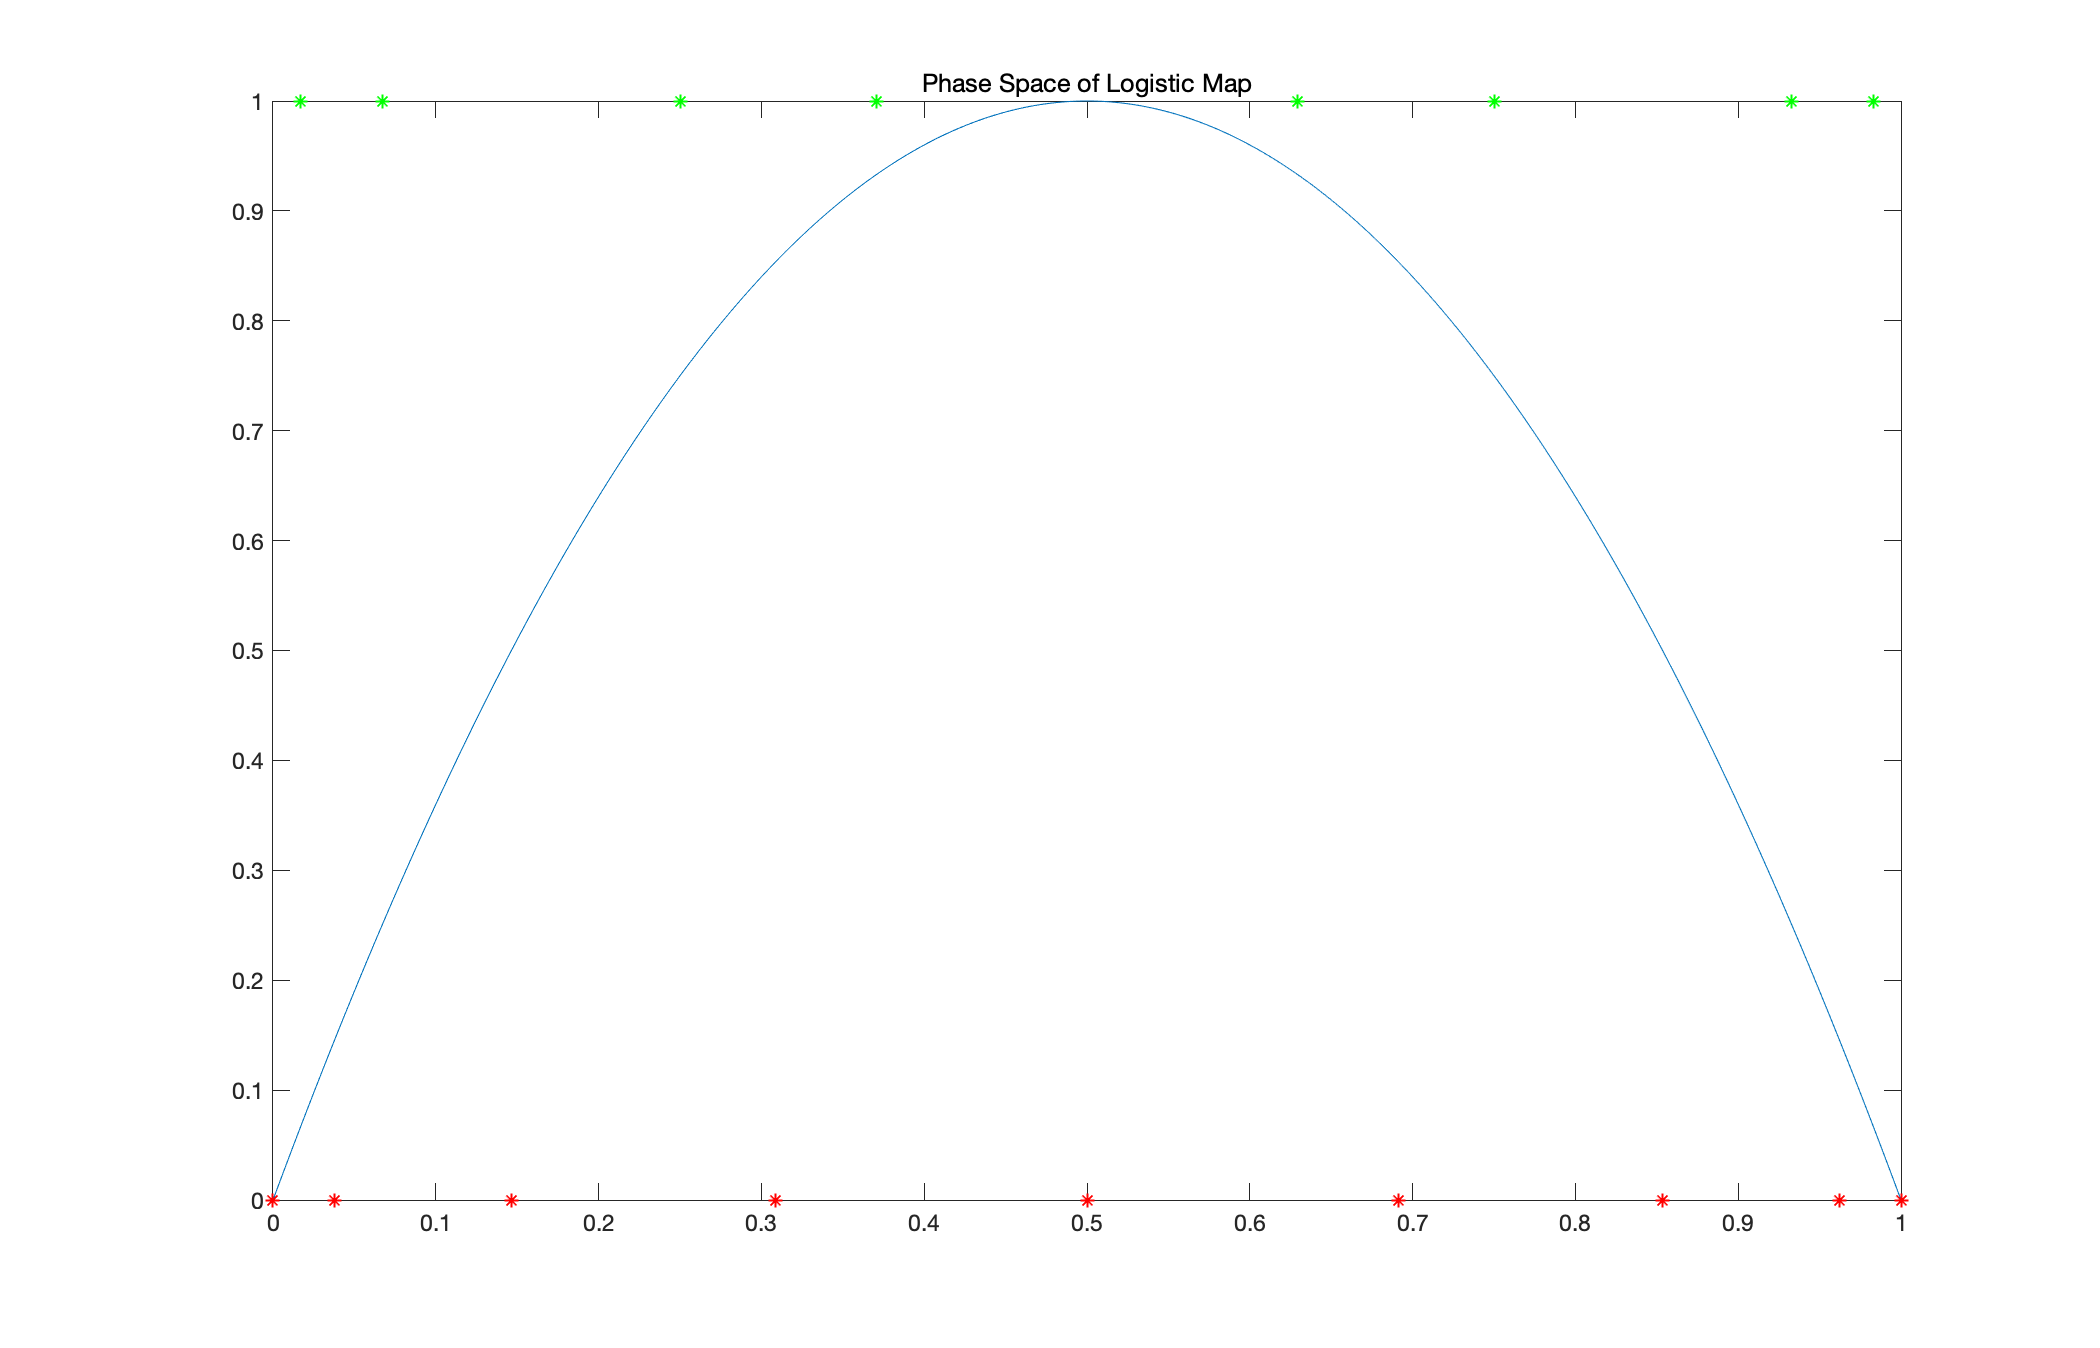
\includegraphics[scale=0.13]{logistic/noise/Logistic_noise_phase_d0}}
    \subfloat[noise=0.001]{
      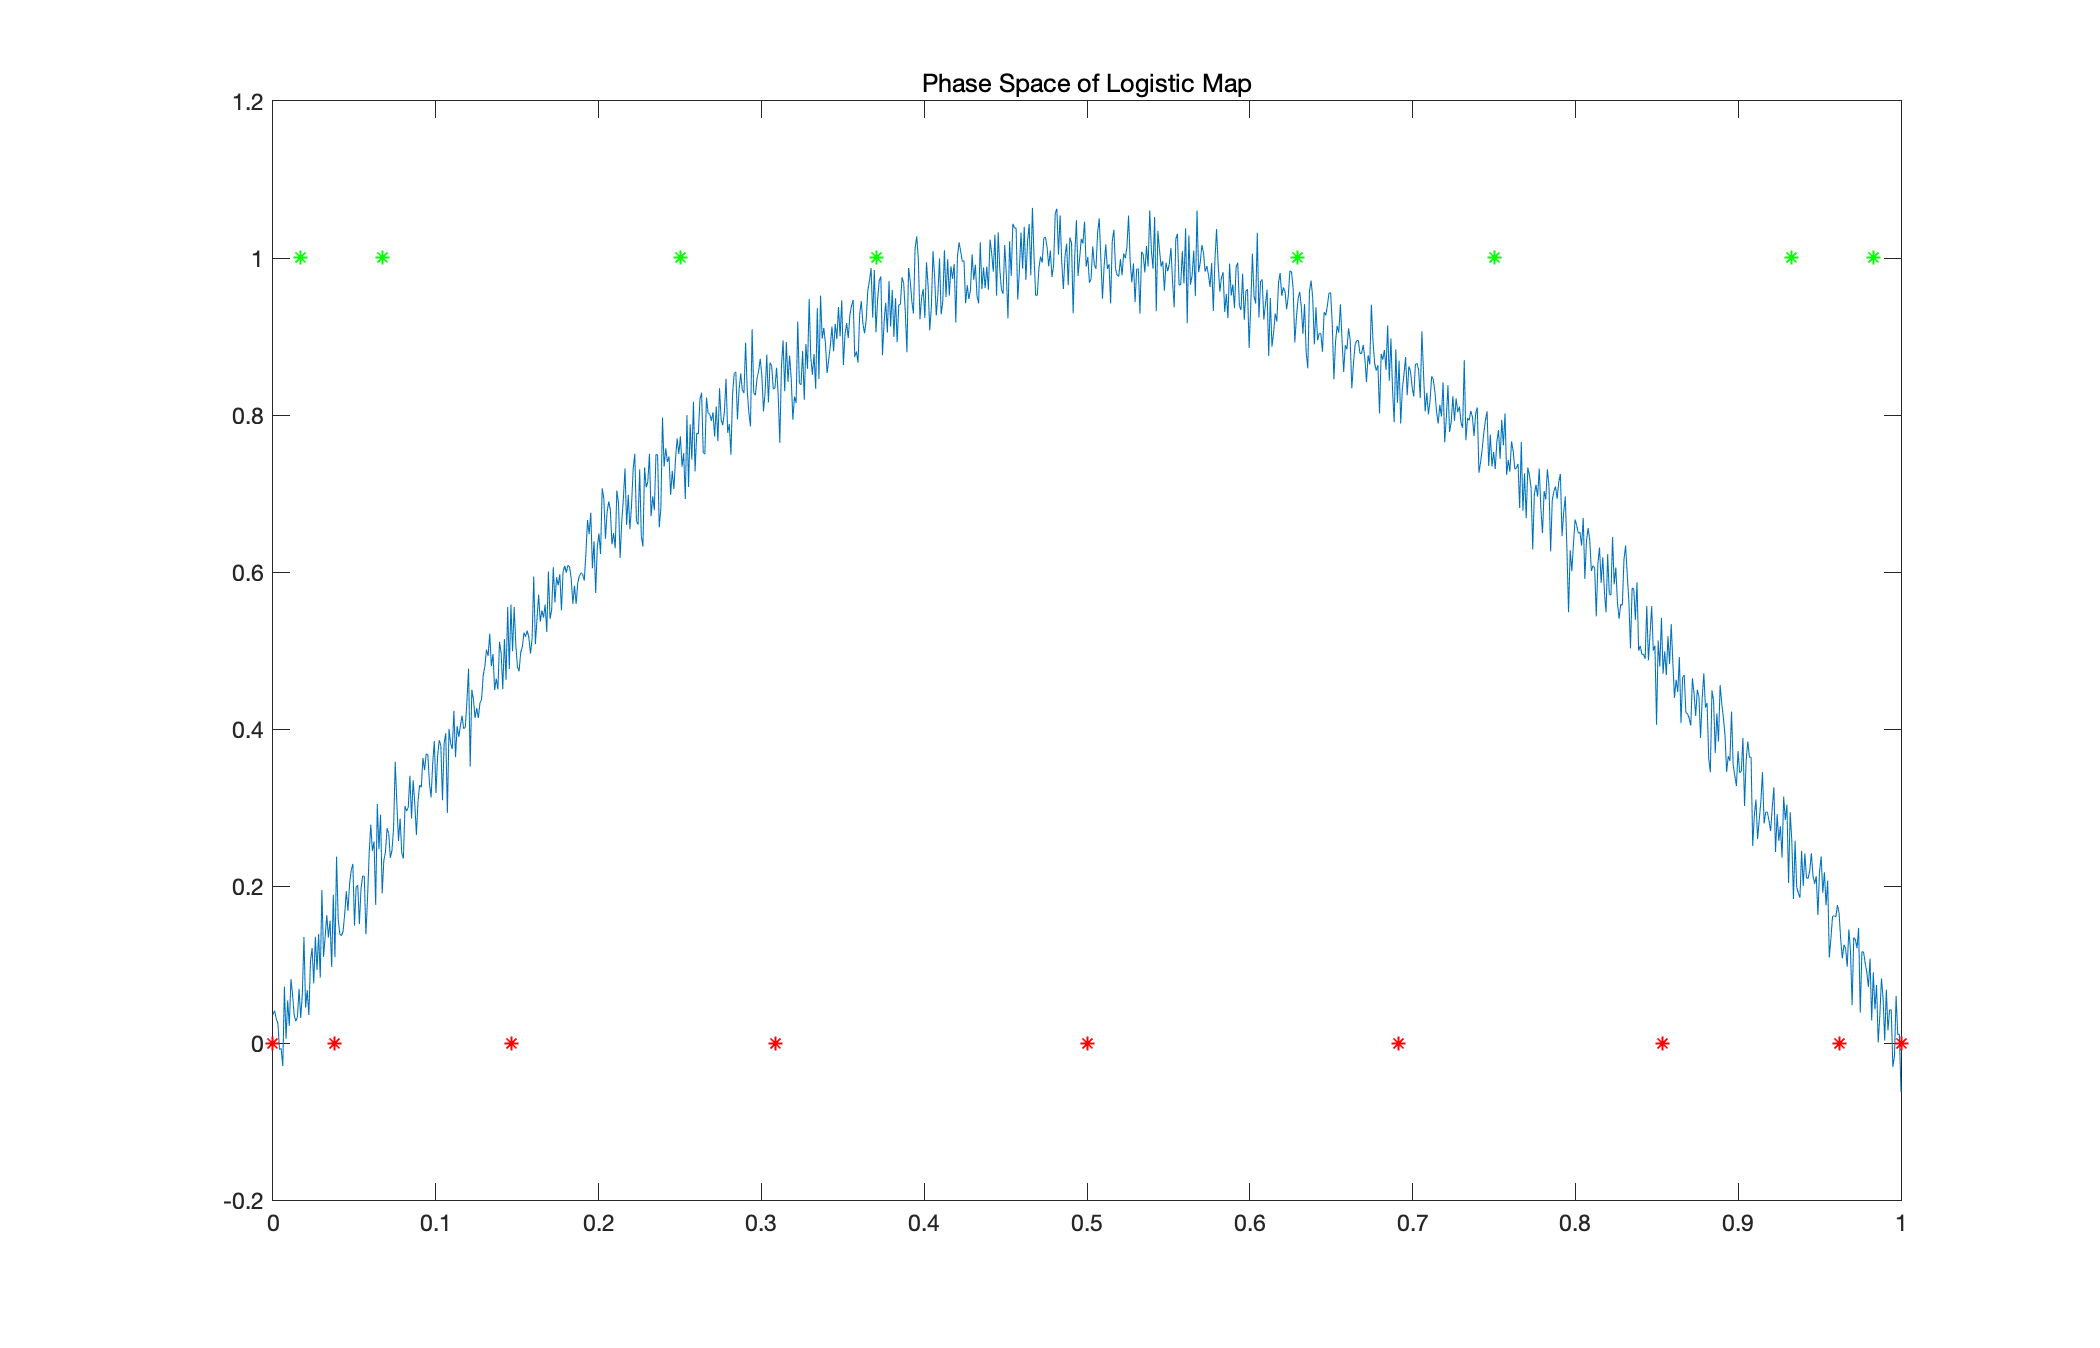
\includegraphics[scale=0.13]{logistic/noise/Logistic_noise_phase_d0-001}}
    \subfloat[noise=0.01]{
      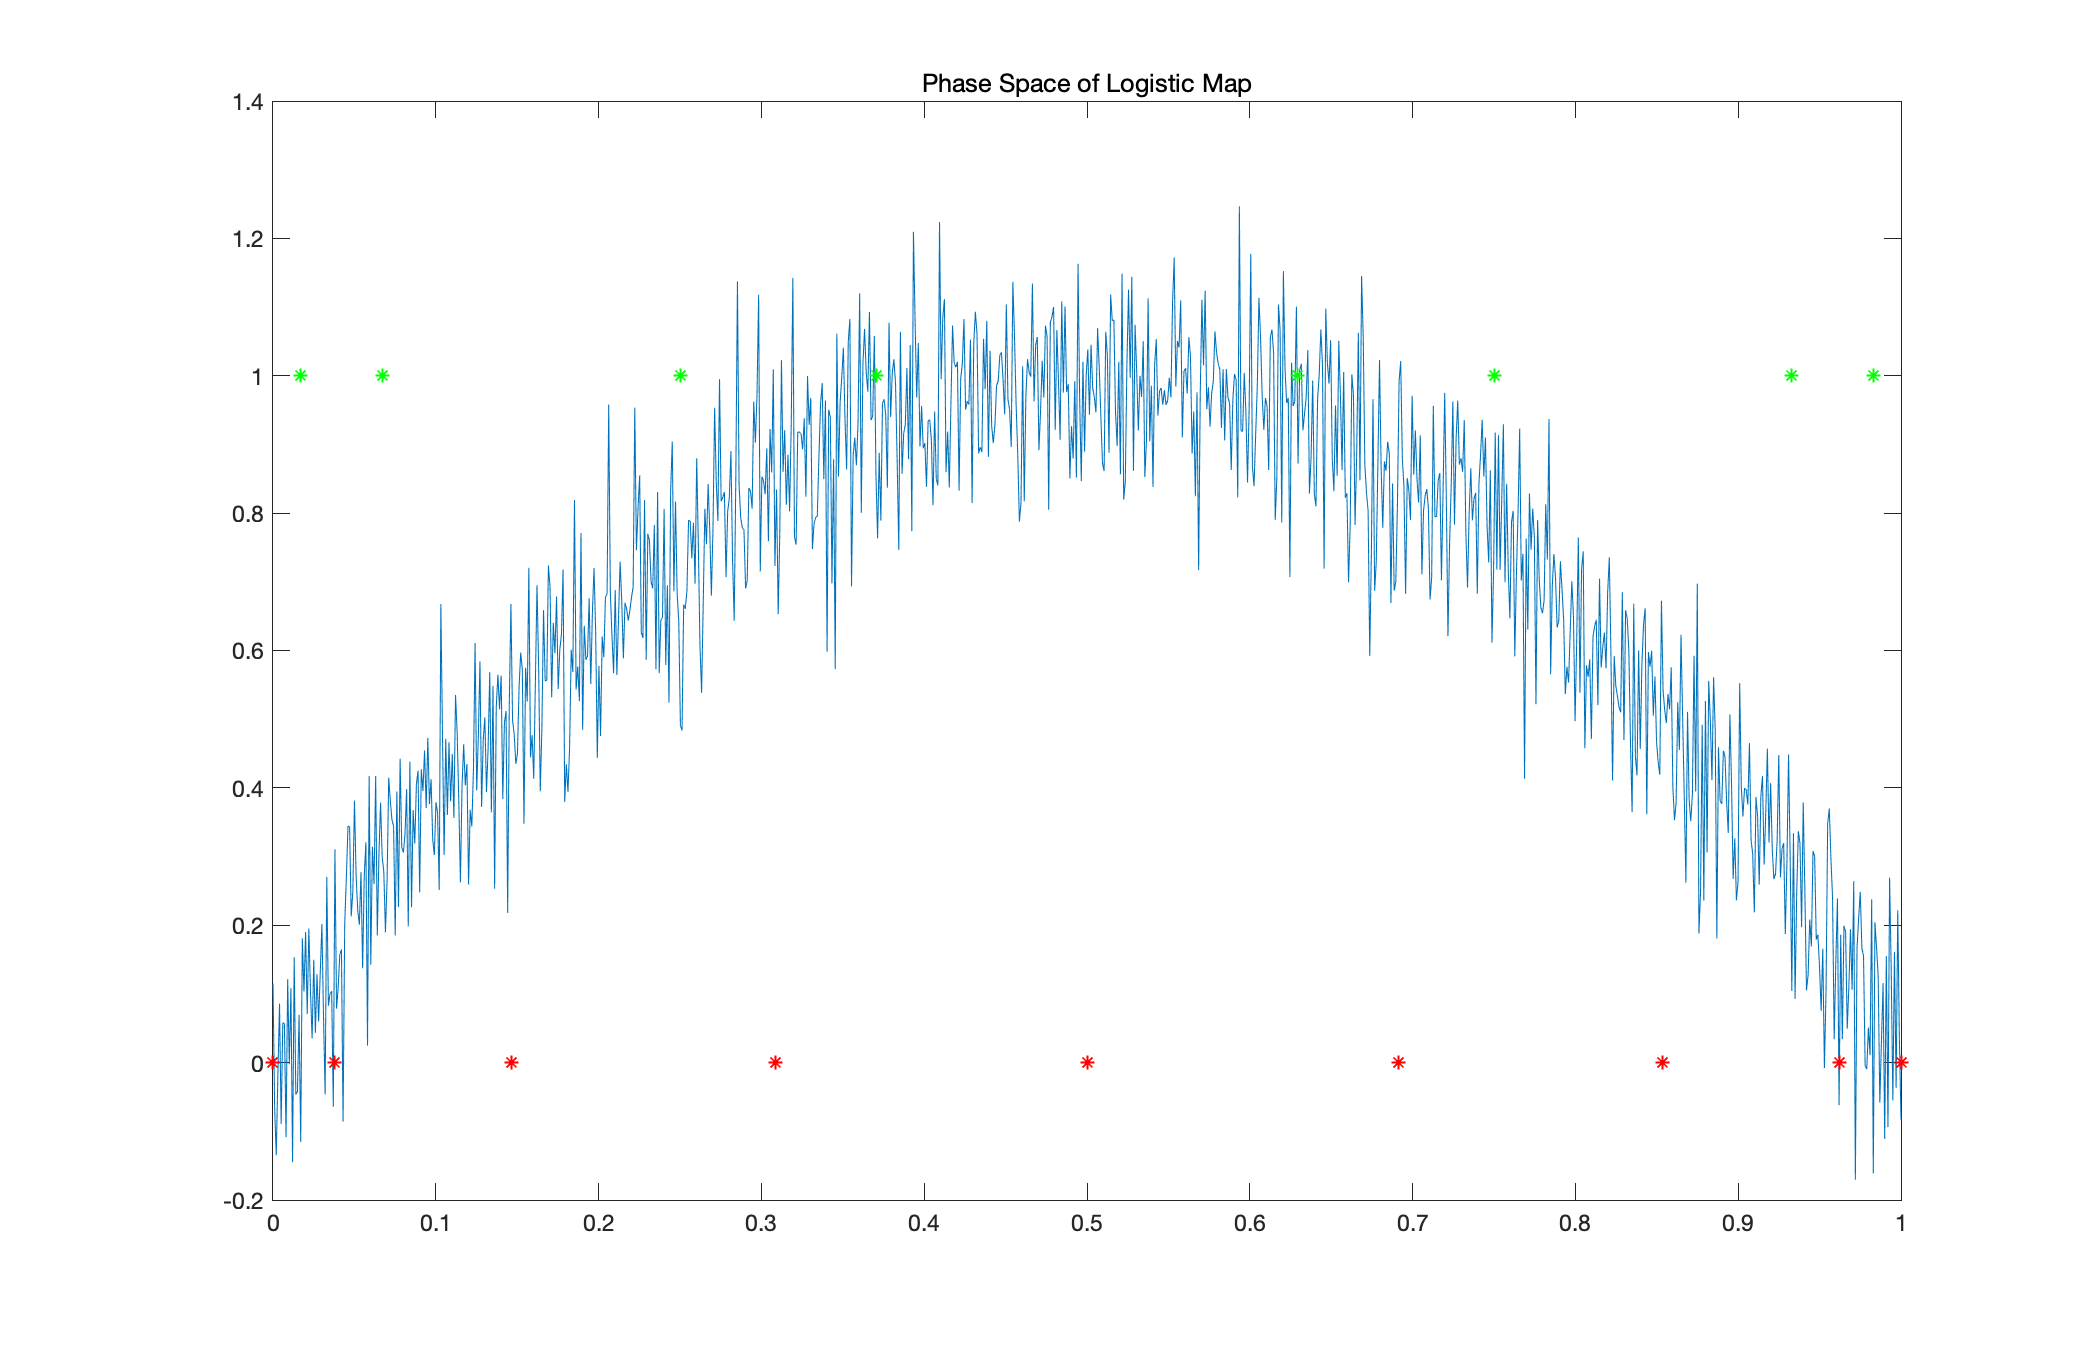
\includegraphics[scale=0.13]{logistic/noise/Logistic_noise_phase_d0-01}}
    \caption{Logistic映射不同噪声下的相空间}
  \end{figure}
  
  \begin{figure}
    \centering%[2,3,4,5,8,10,15,20]
    \subfloat[m=2]{
      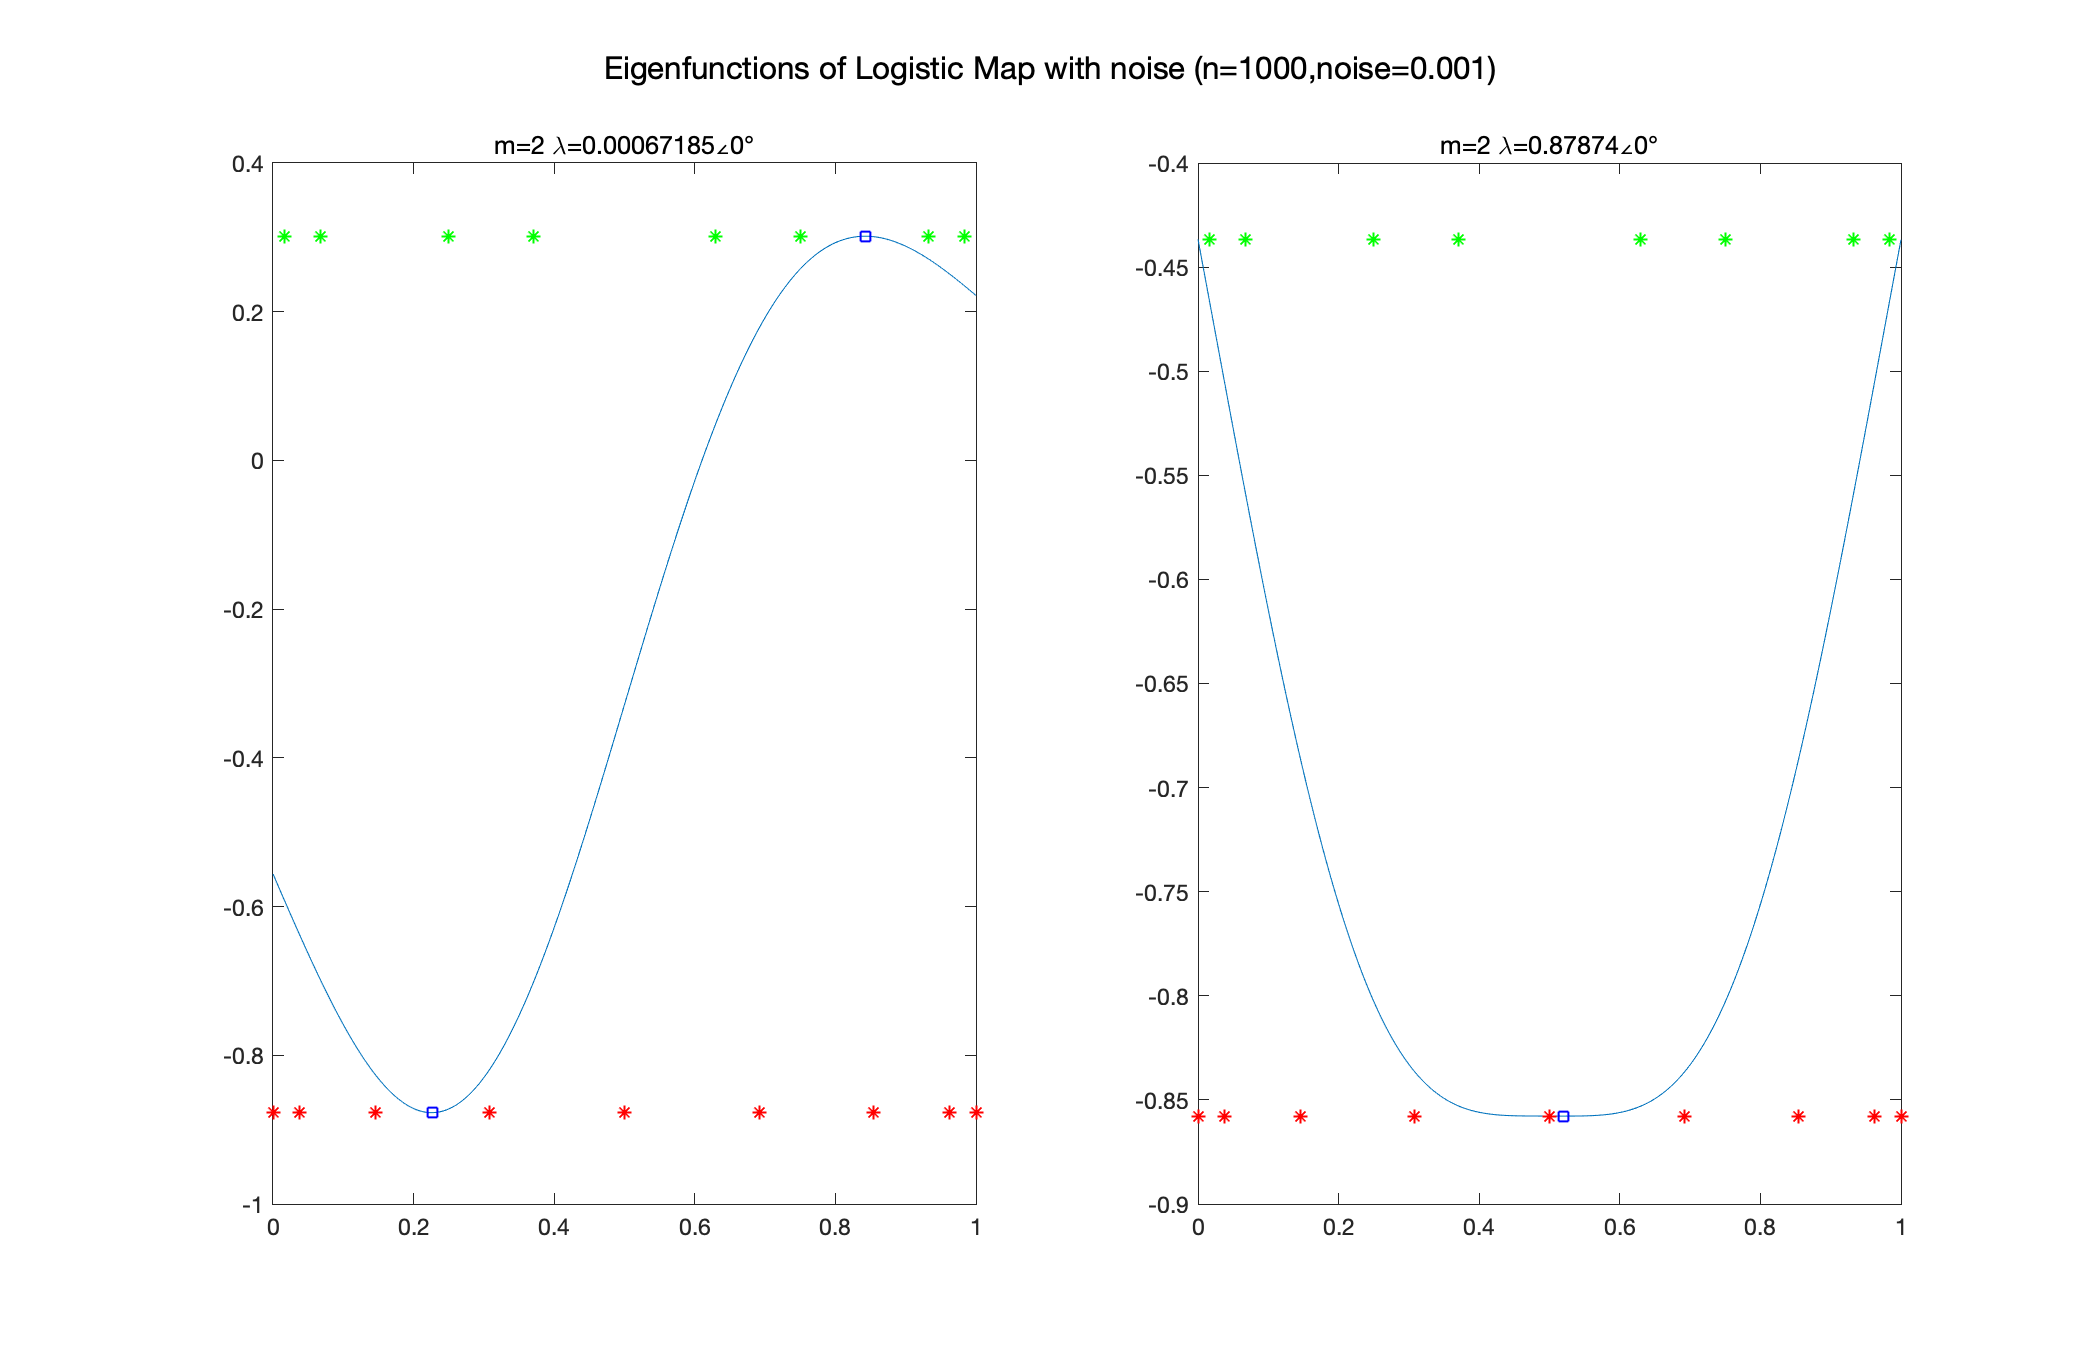
\includegraphics[scale=0.2]{logistic/noise/Logistic_eigen_noise_n1000m2d0-001}}
    \subfloat[m=3]{
      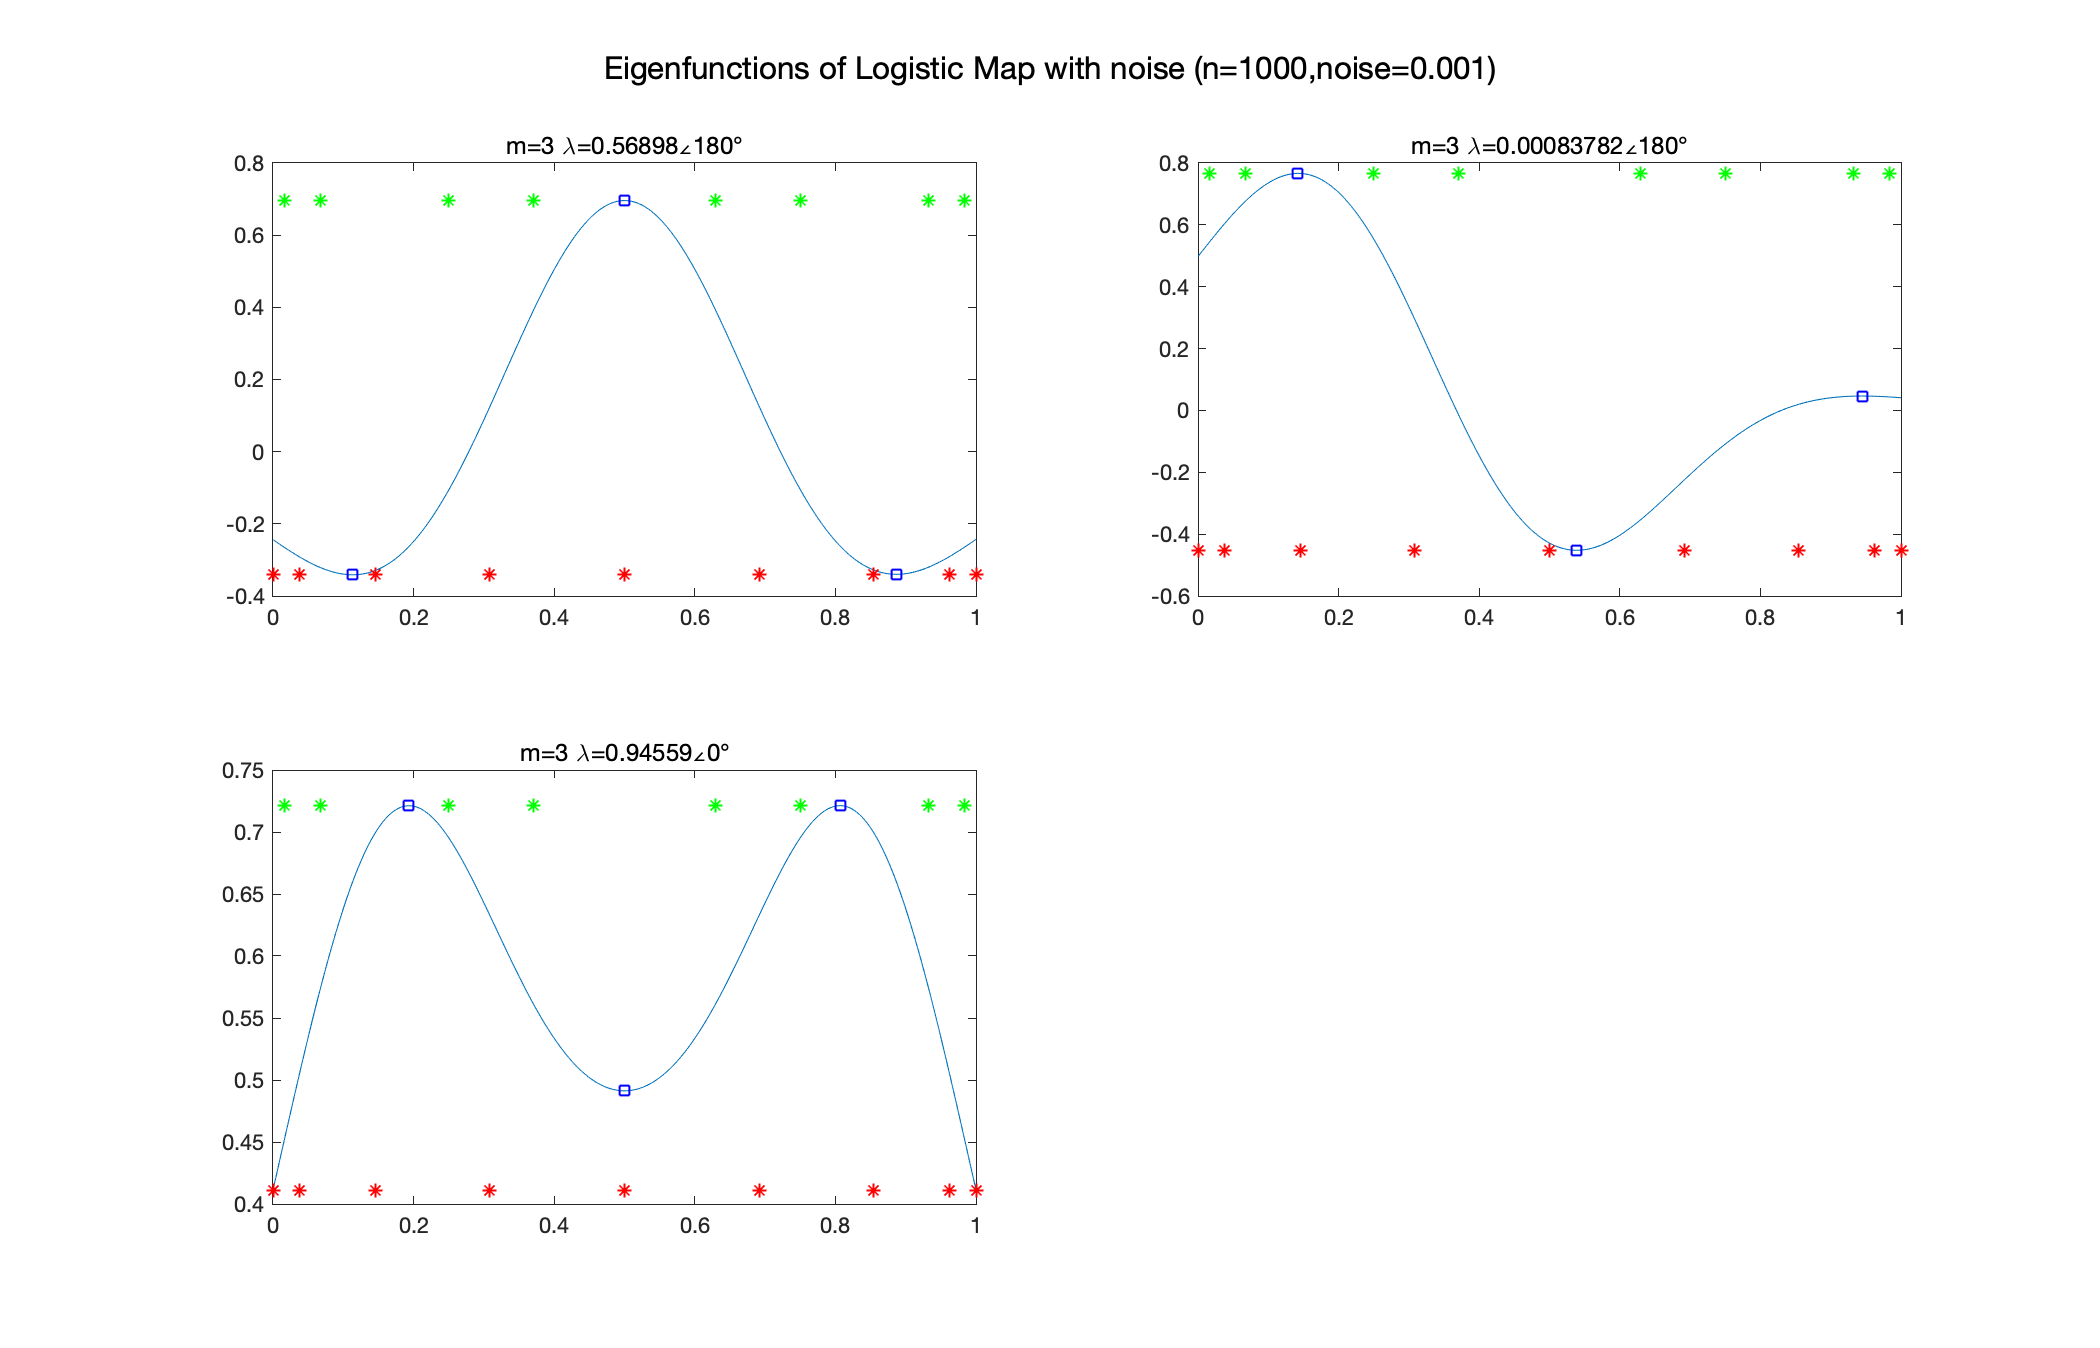
\includegraphics[scale=0.2]{logistic/noise/Logistic_eigen_noise_n1000m3d0-001}}
      \\
    \subfloat[m=4]{
      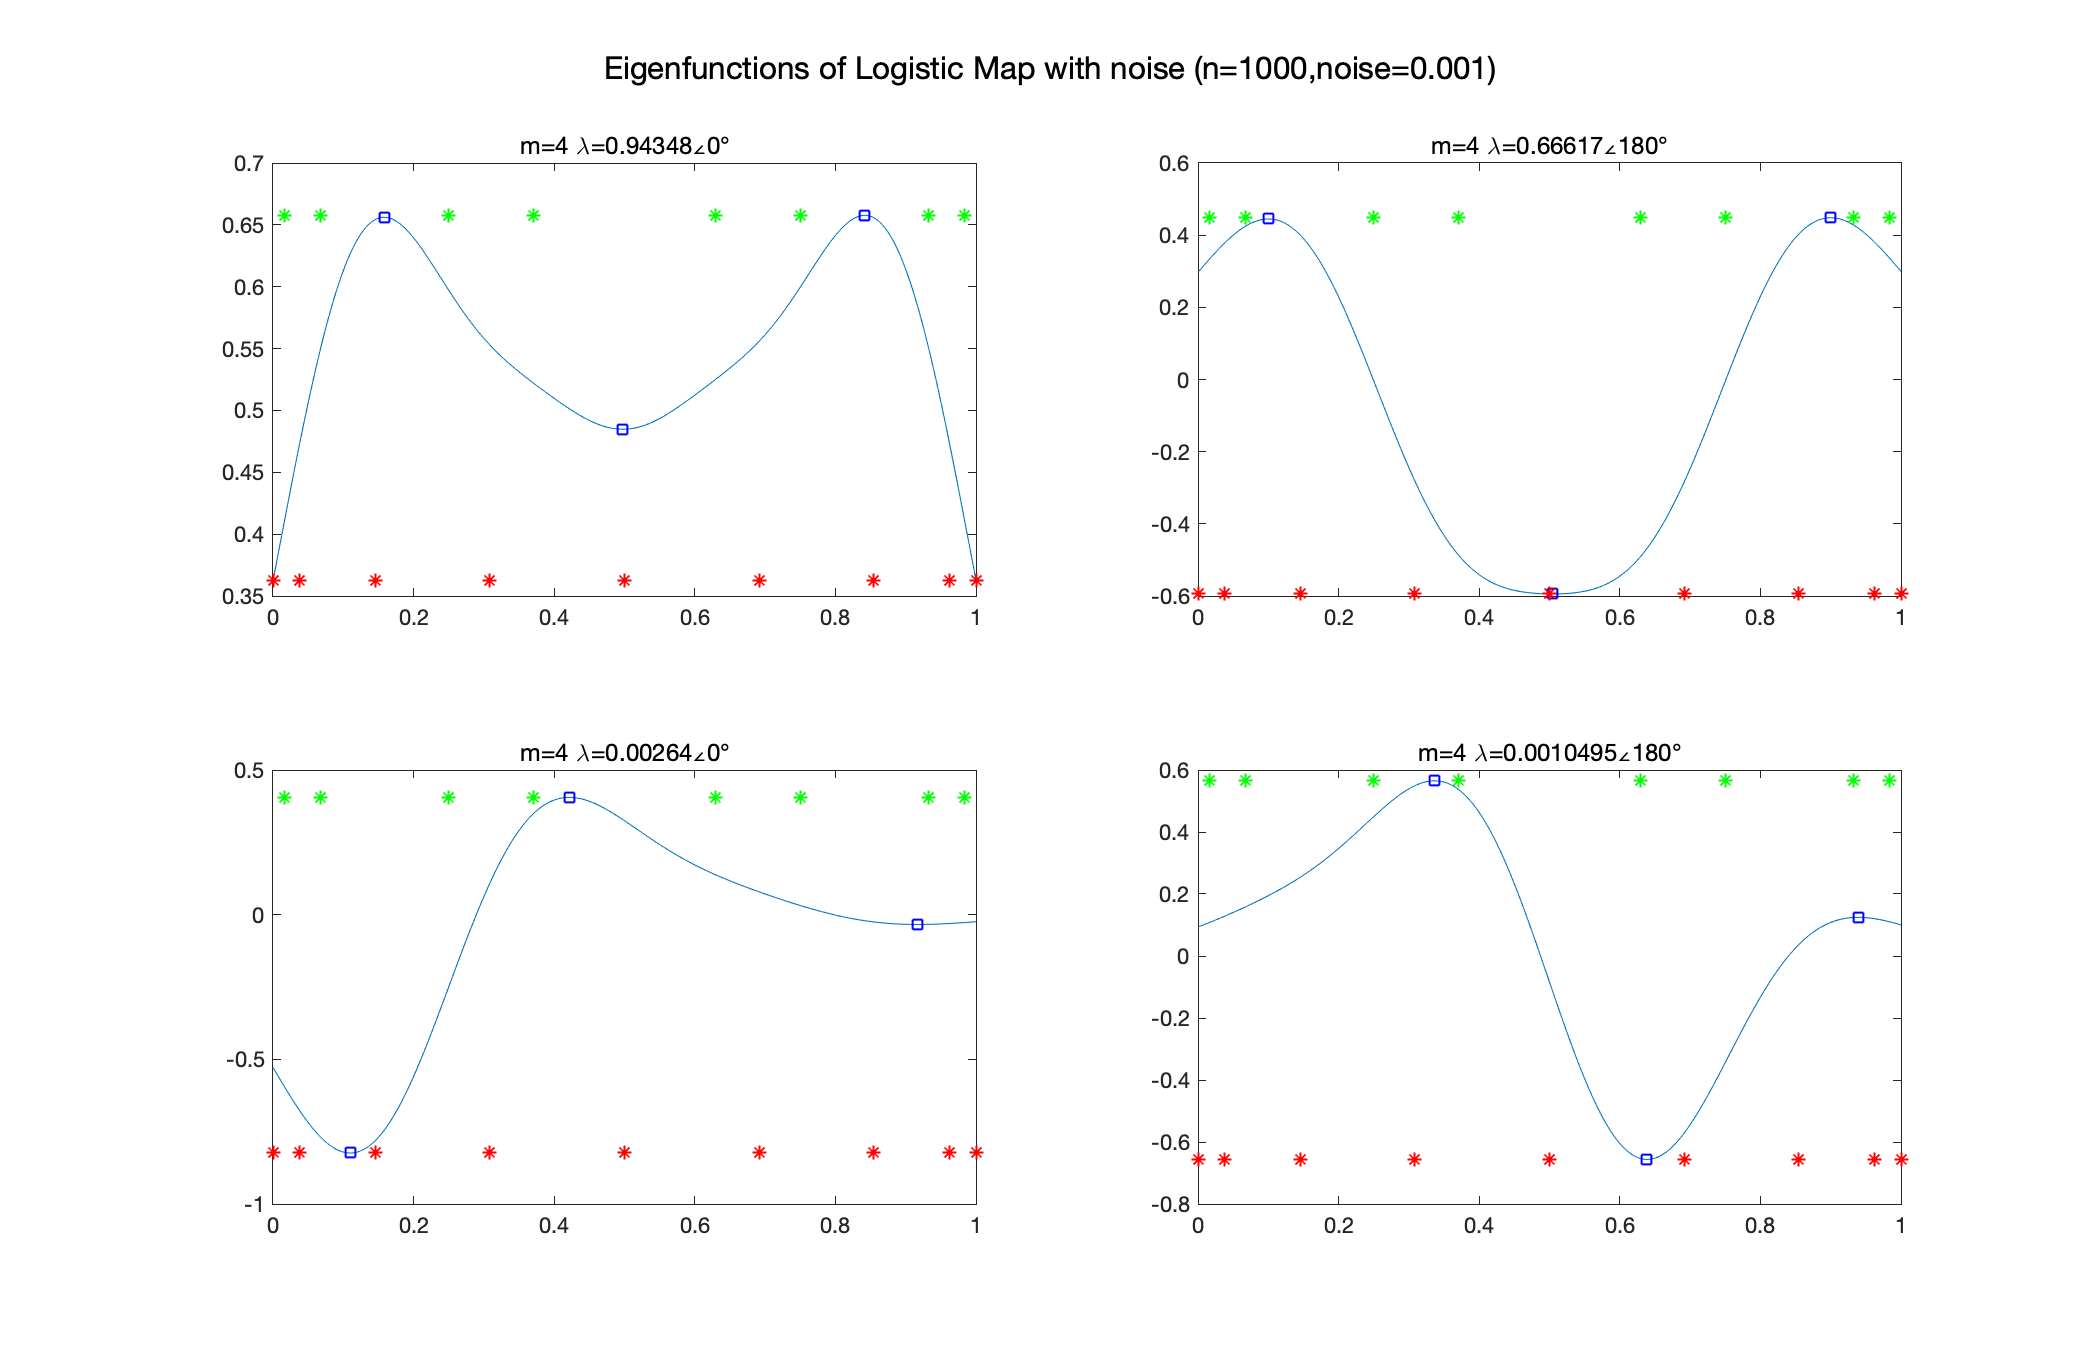
\includegraphics[scale=0.2]{logistic/noise/Logistic_eigen_noise_n1000m4d0-001}}
    \subfloat[m=5]{
      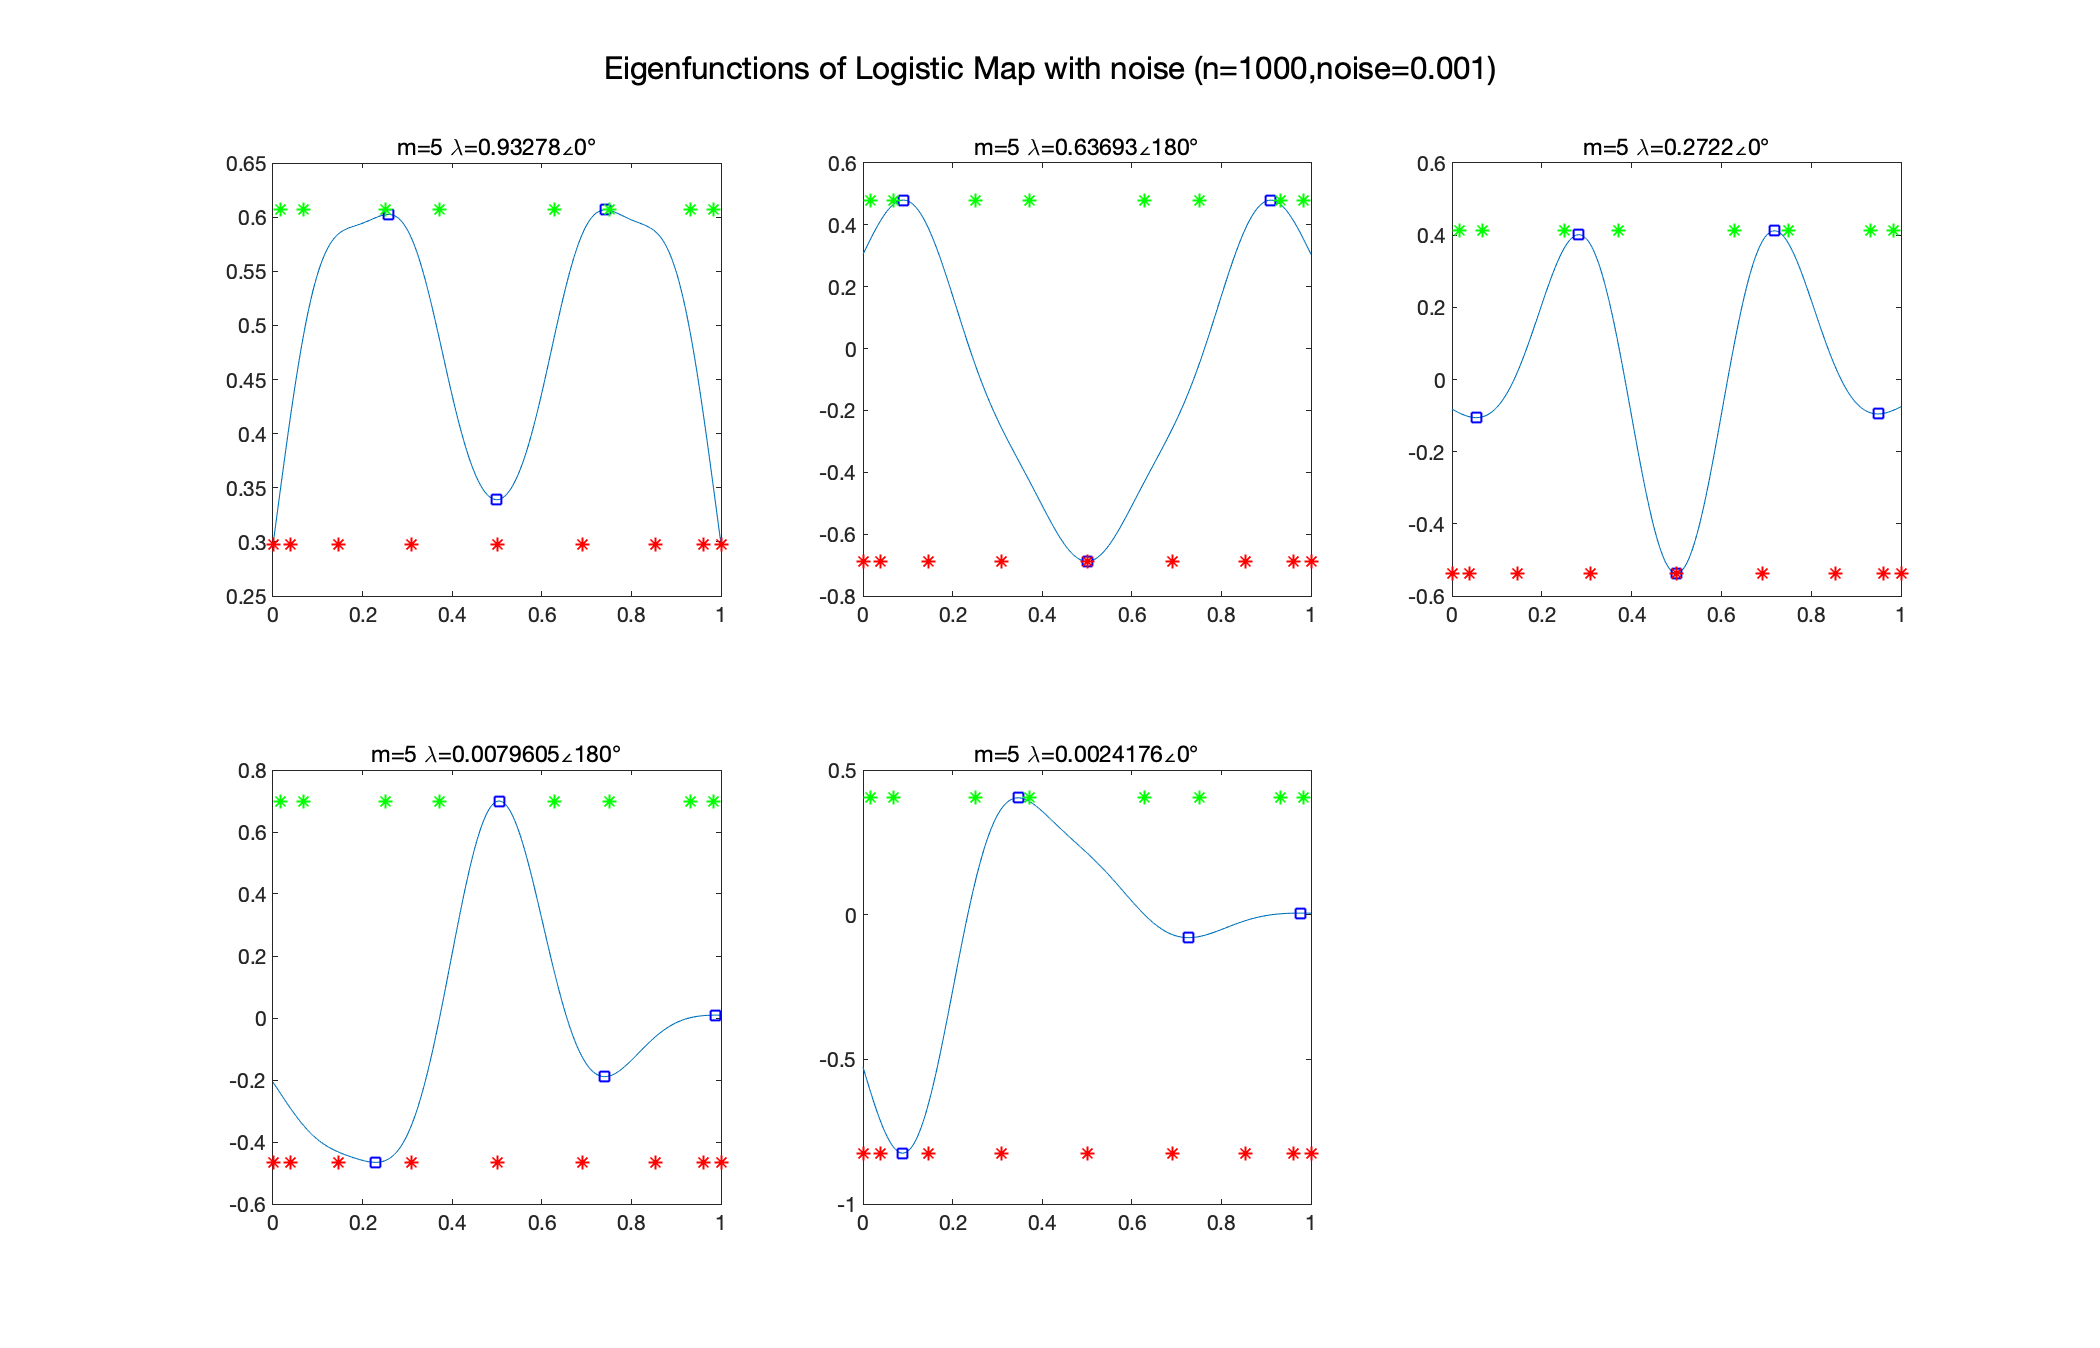
\includegraphics[scale=0.2]{logistic/noise/Logistic_eigen_noise_n1000m5d0-001}}
      \\
    \subfloat[m=8]{
      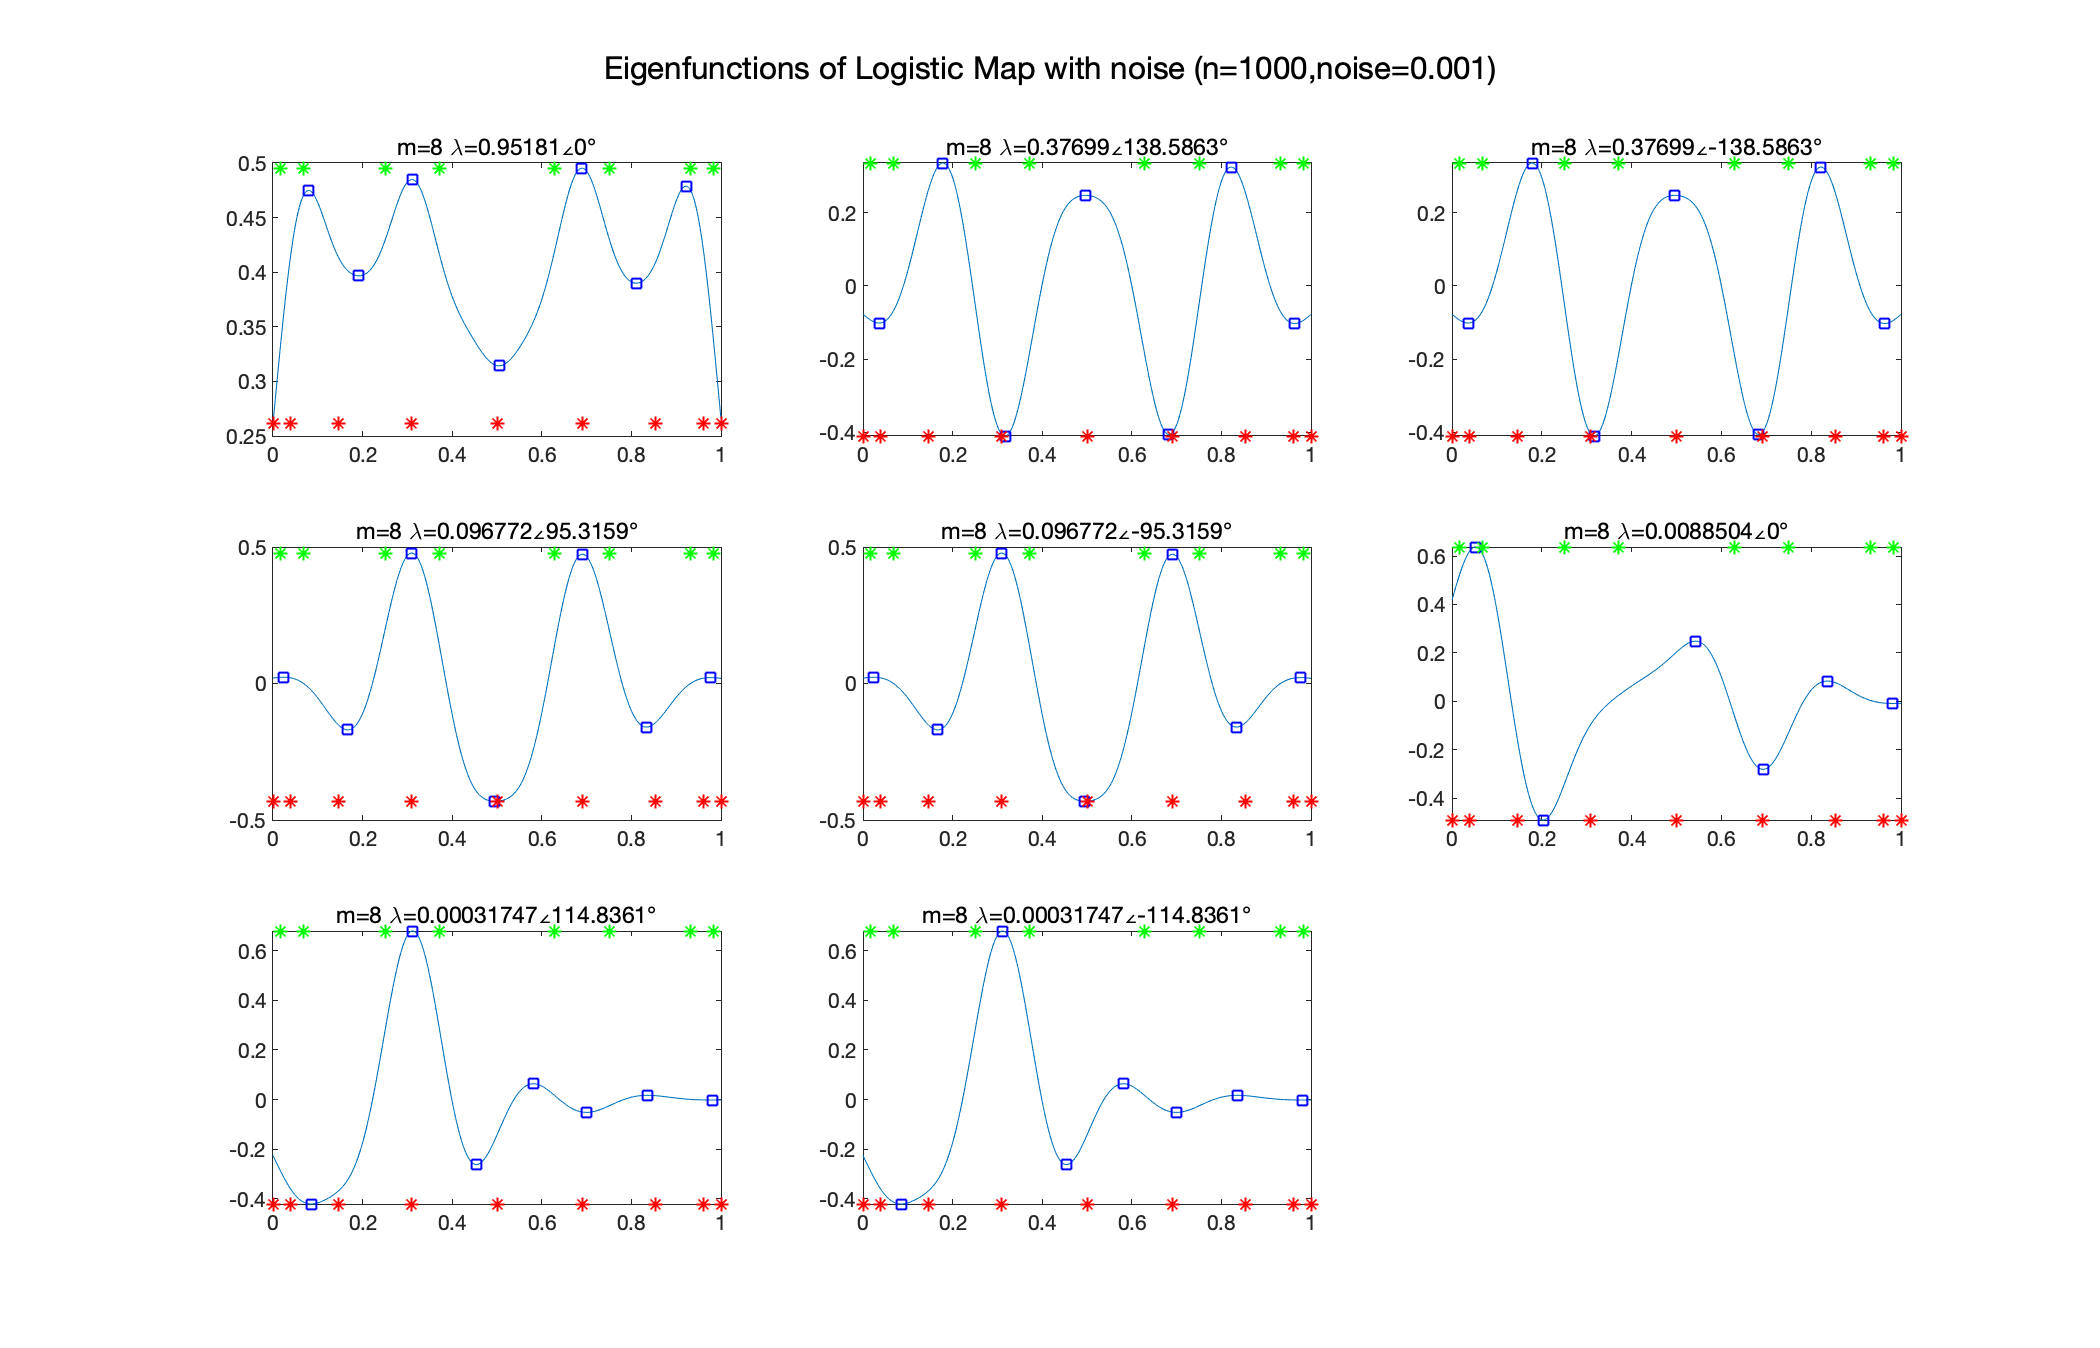
\includegraphics[scale=0.2]{logistic/noise/Logistic_eigen_noise_n1000m8d0-001}}
    \subfloat[m=10]{
      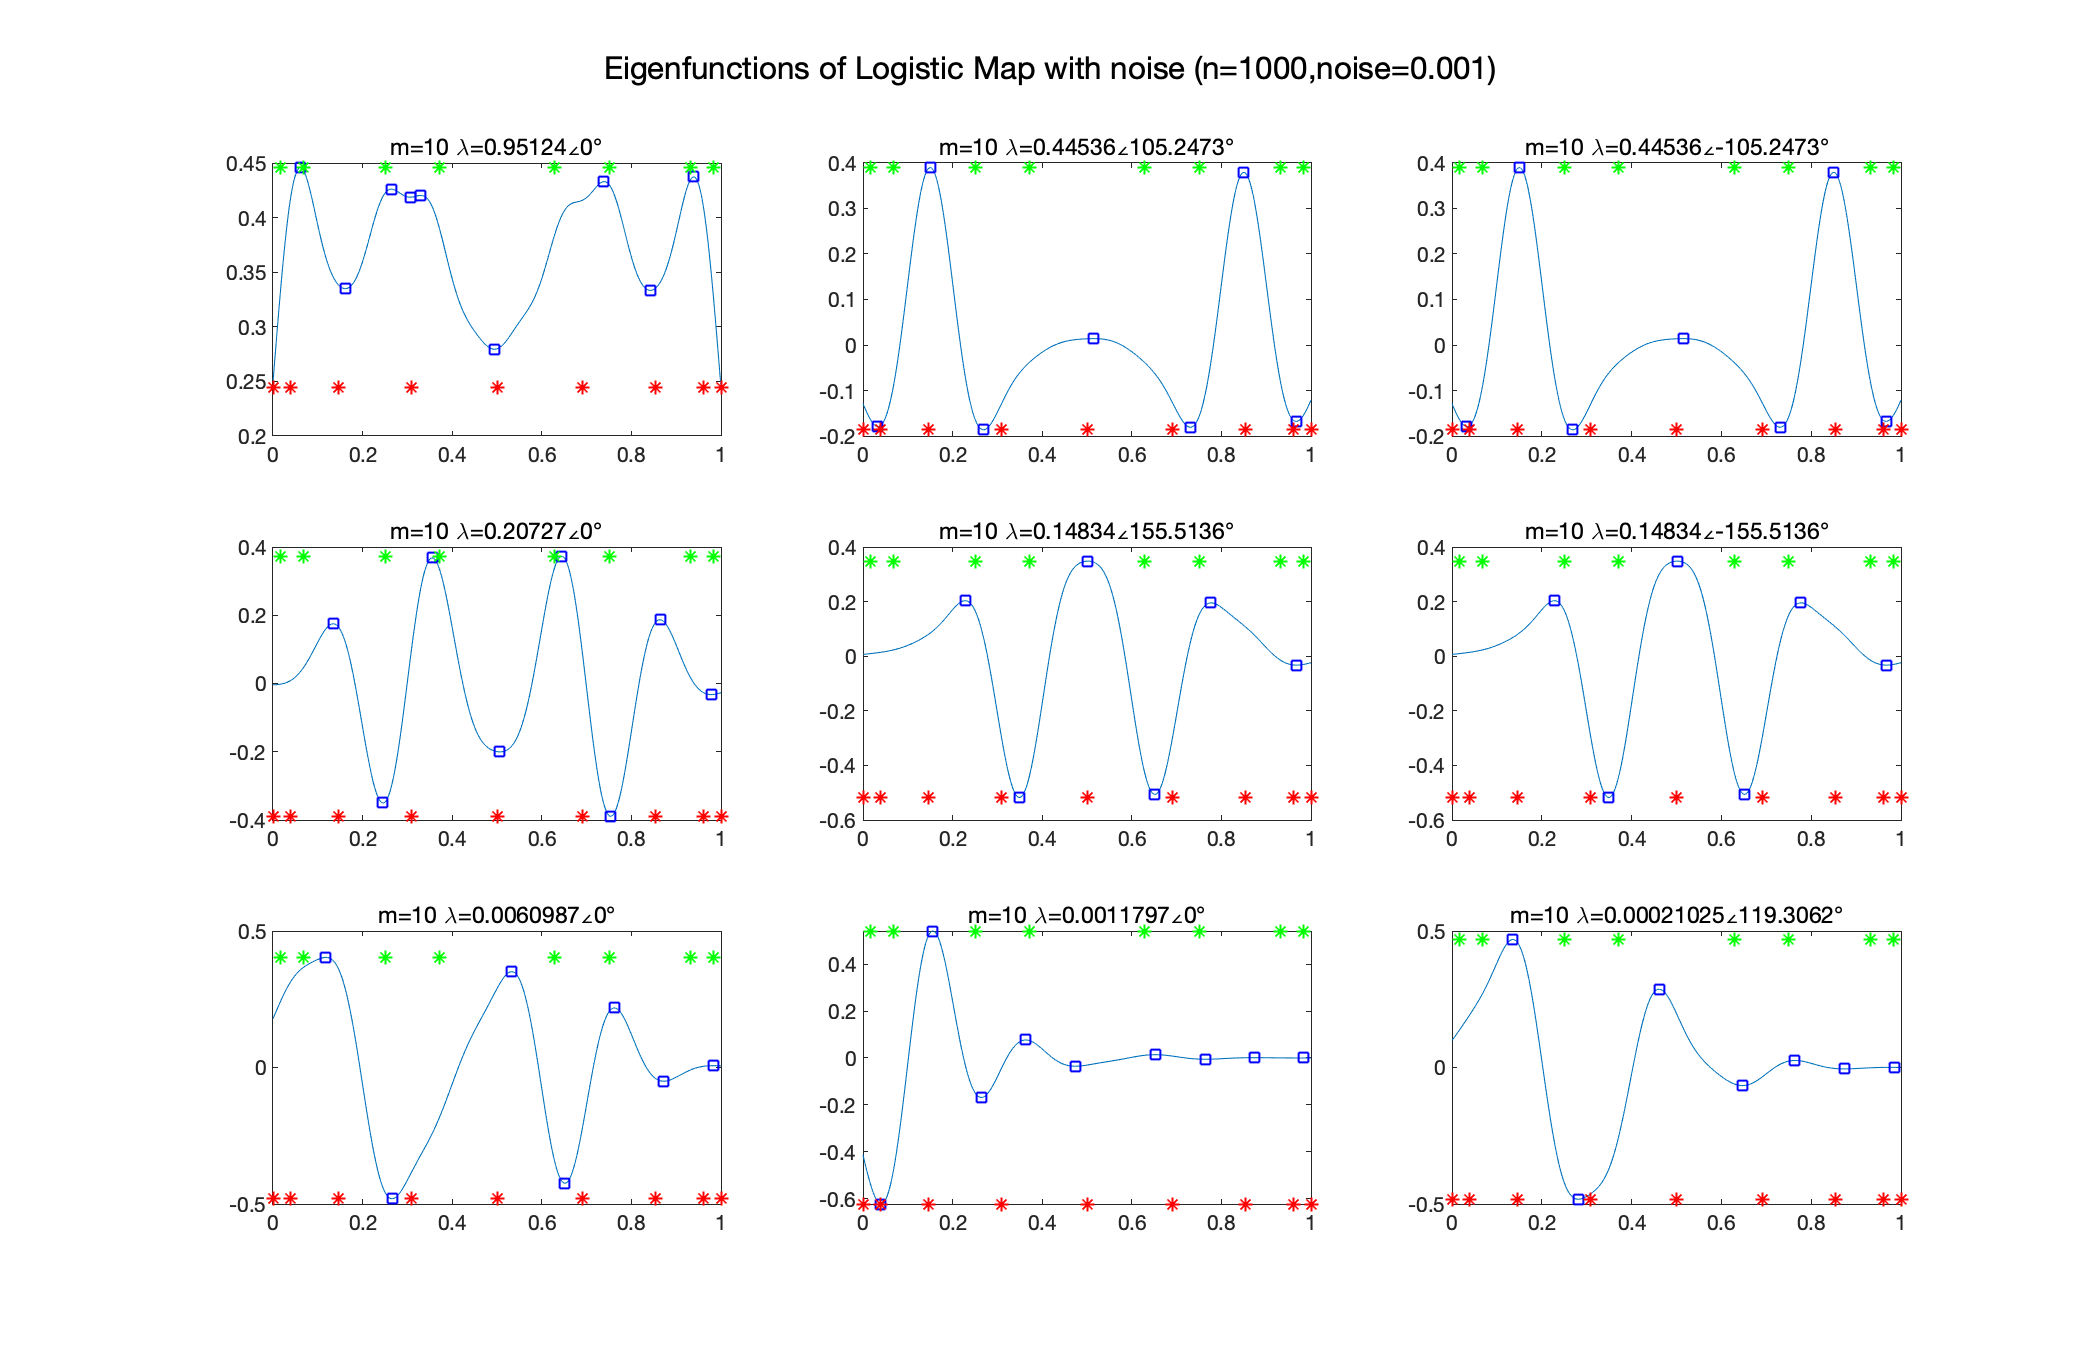
\includegraphics[scale=0.2]{logistic/noise/Logistic_eigen_noise_n1000m10d0-001}}
      \\
    \subfloat[m=15]{
      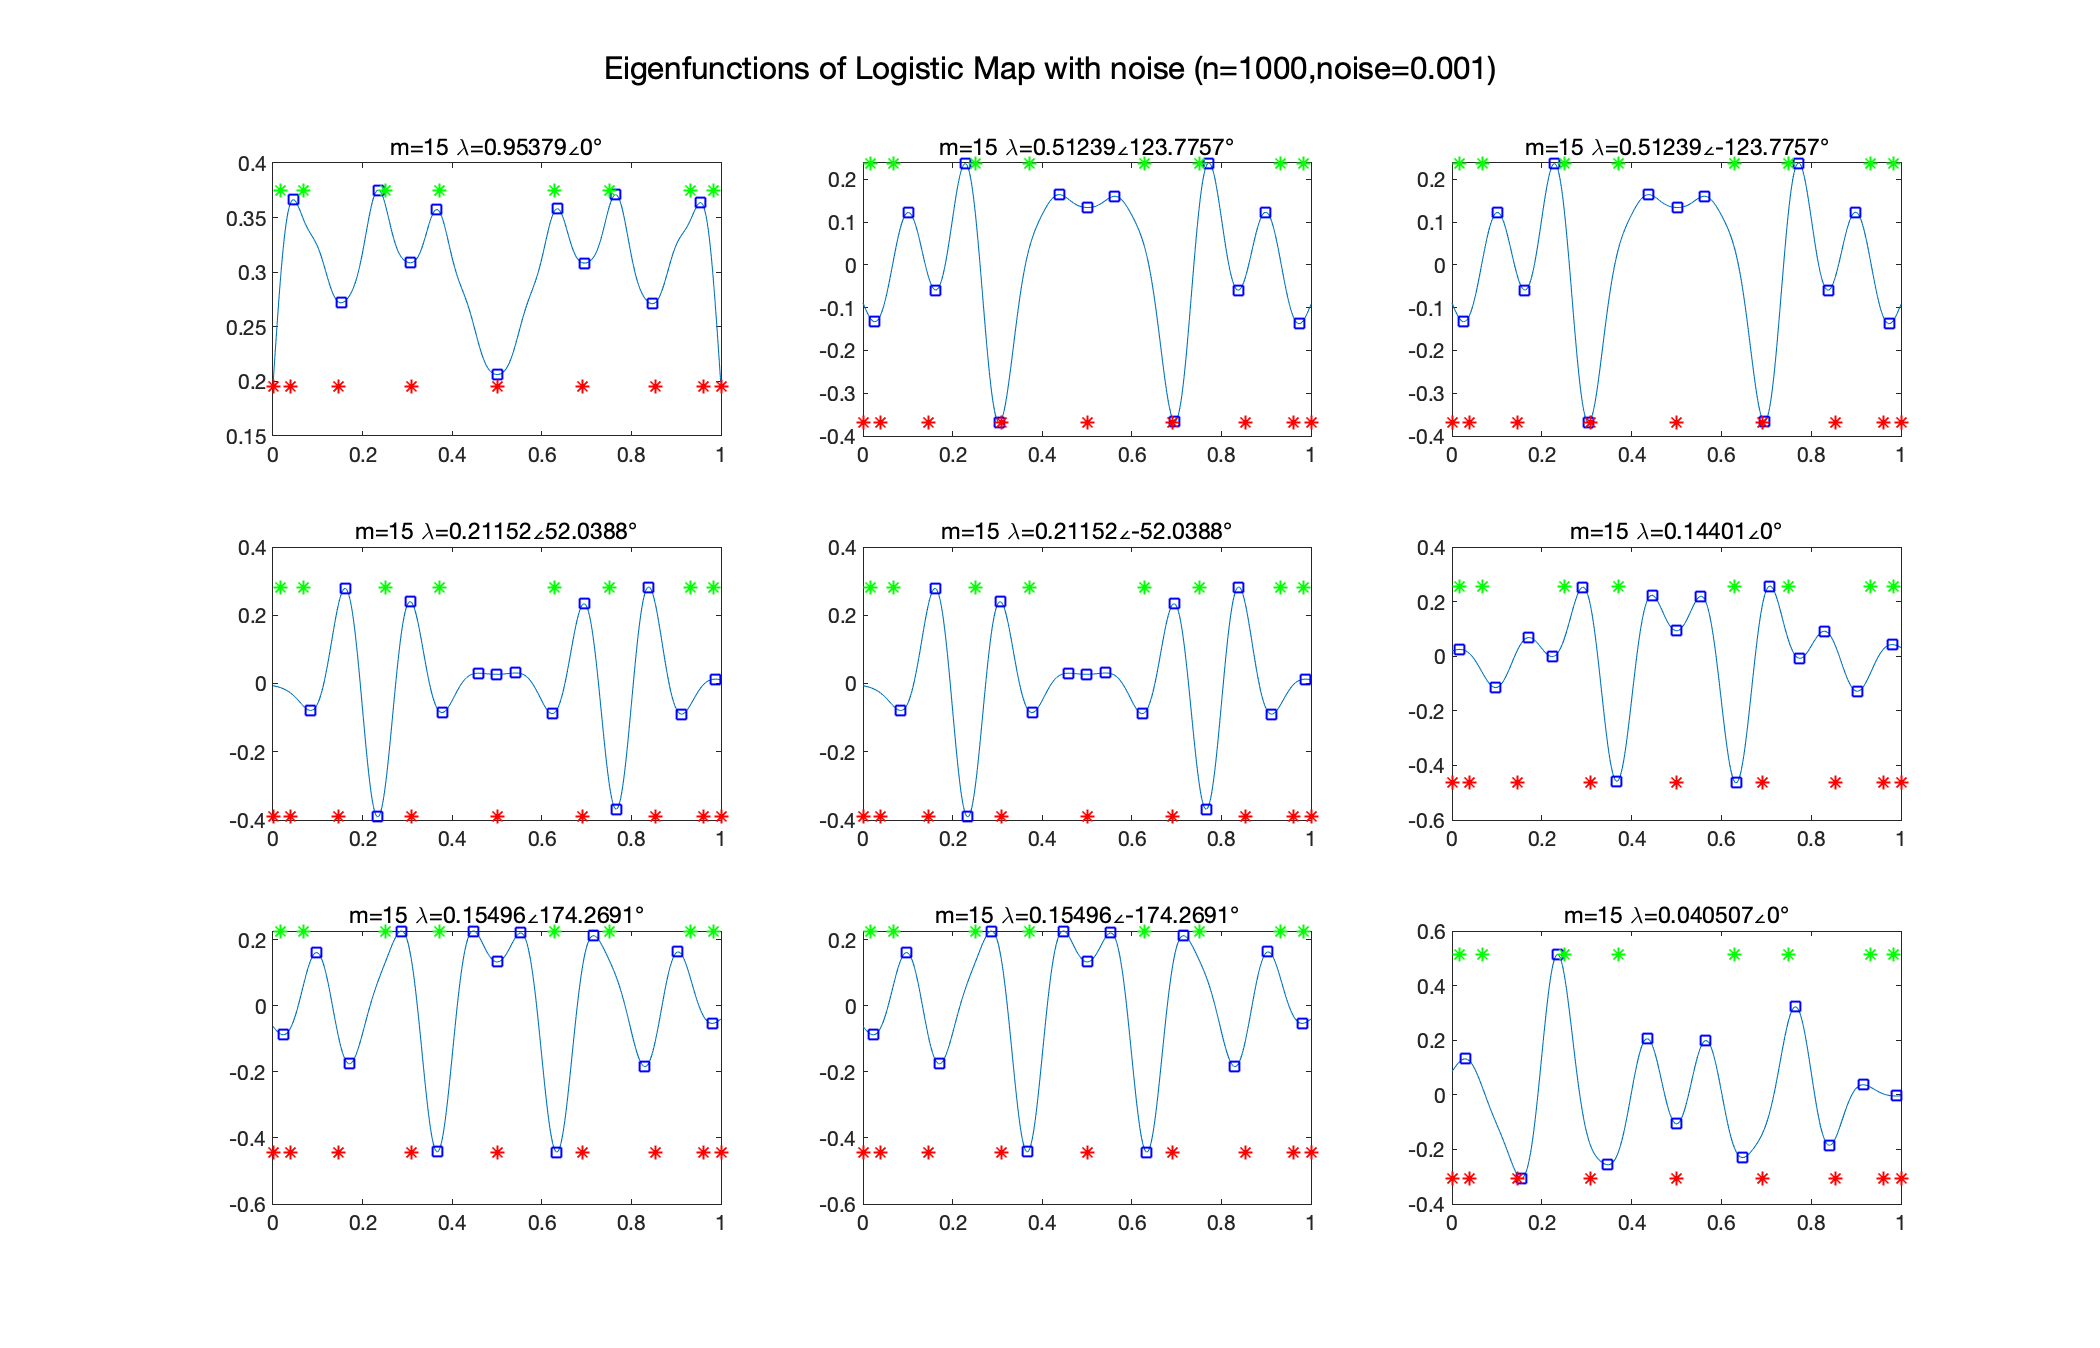
\includegraphics[scale=0.2]{logistic/noise/Logistic_eigen_noise_n1000m15d0-001}}
    \subfloat[m=20]{
      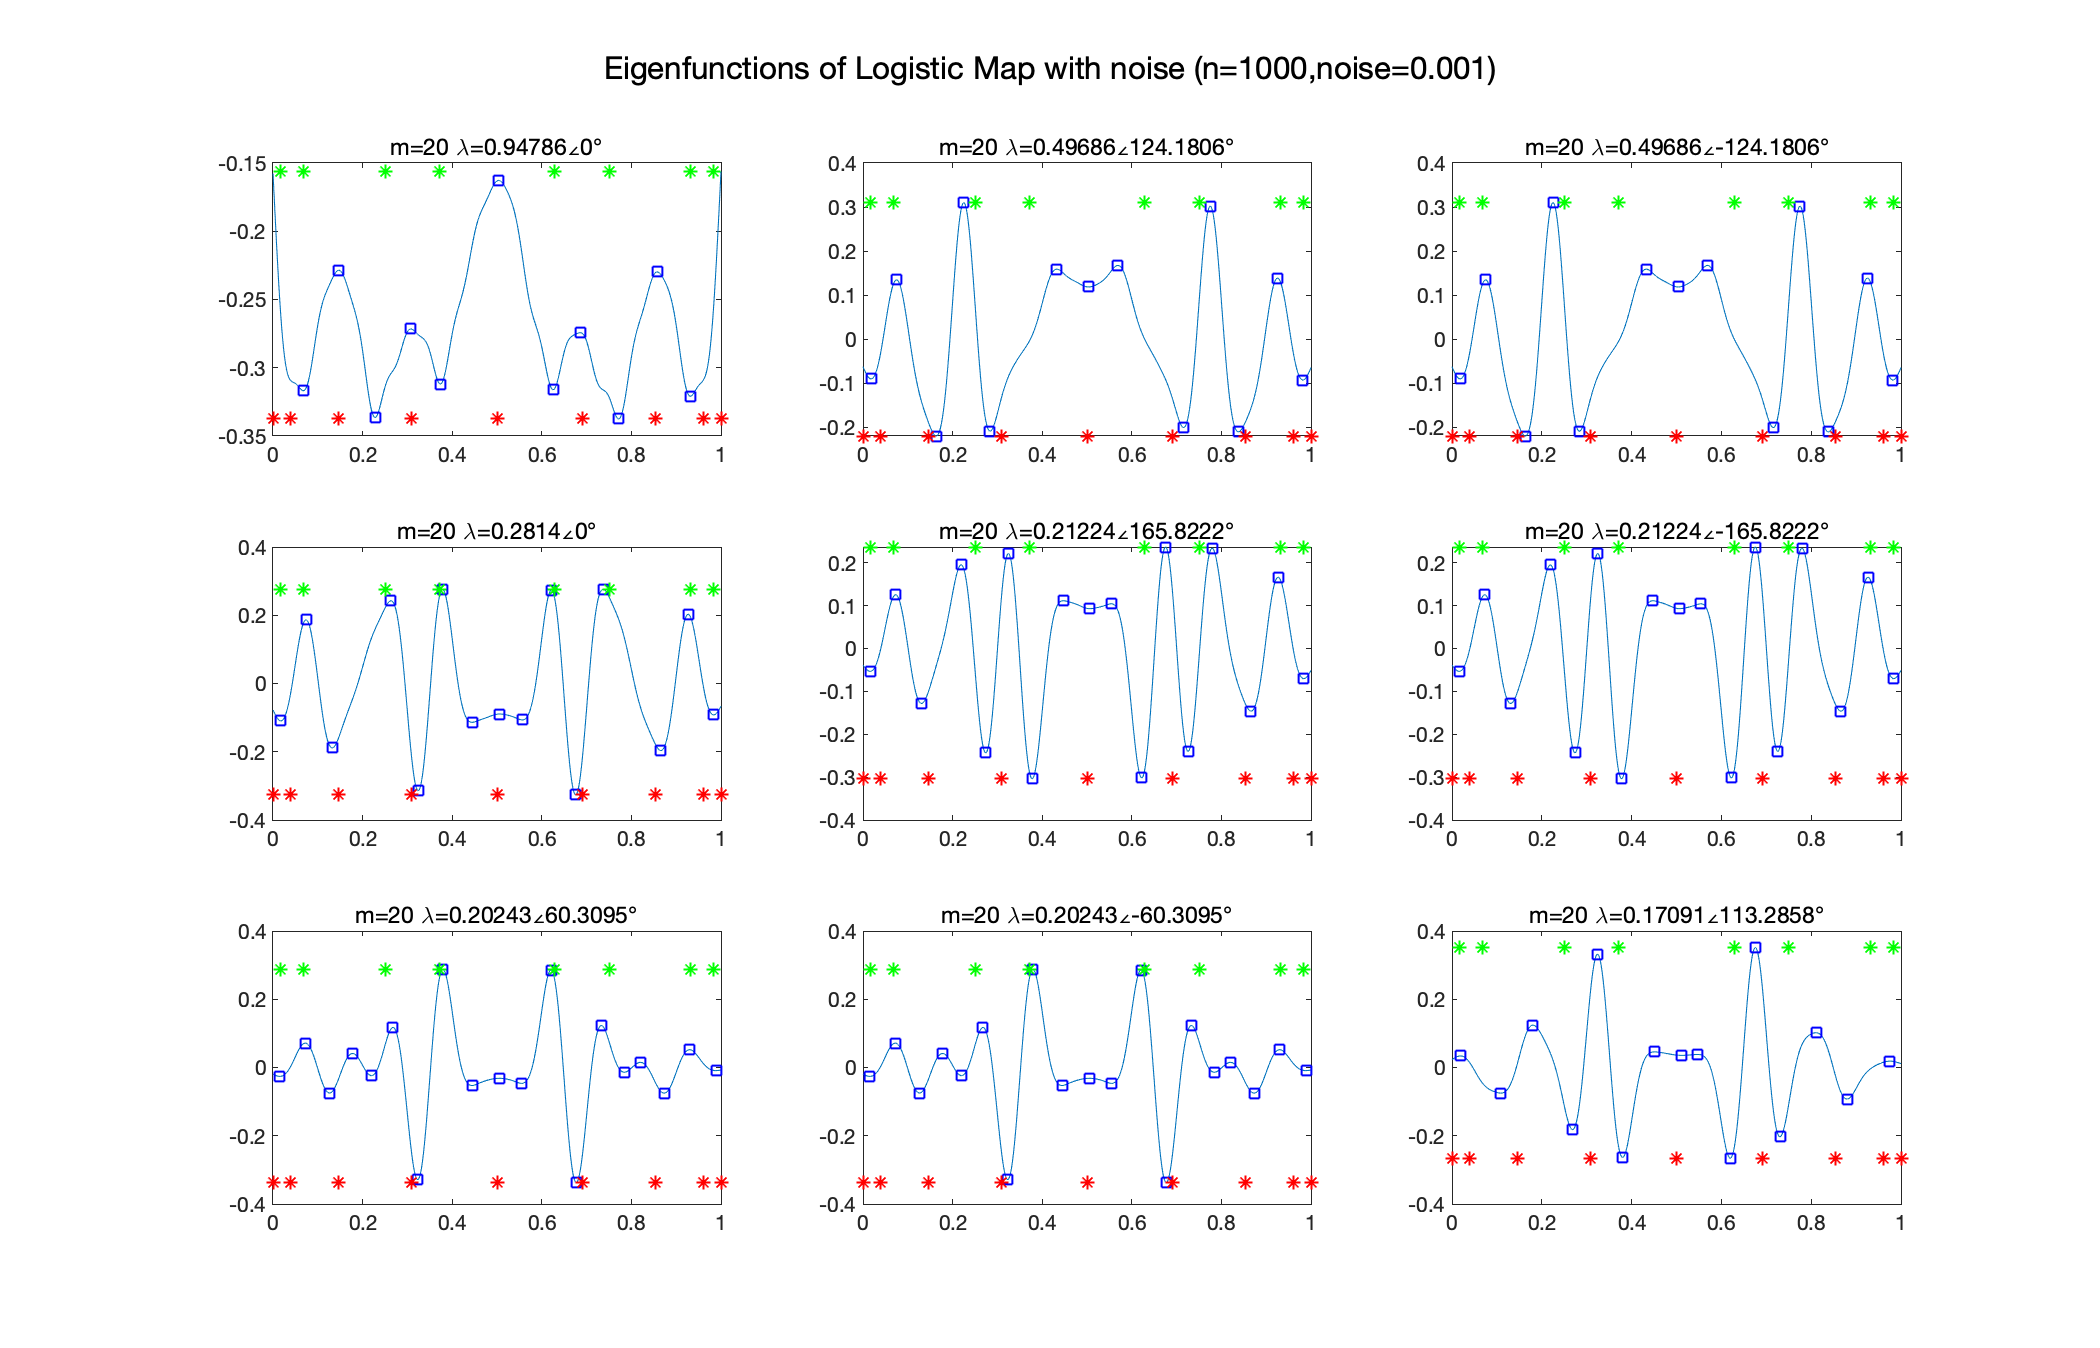
\includegraphics[scale=0.2]{logistic/noise/Logistic_eigen_noise_n1000m20d0-001}}
      \\
    \caption{Logistic射的边界点与本征函数($noise=0.001$)}
  \end{figure}
  
  \begin{figure}
    \centering%[2,3,4,5,8,10,15,20]
    \subfloat[m=2]{
      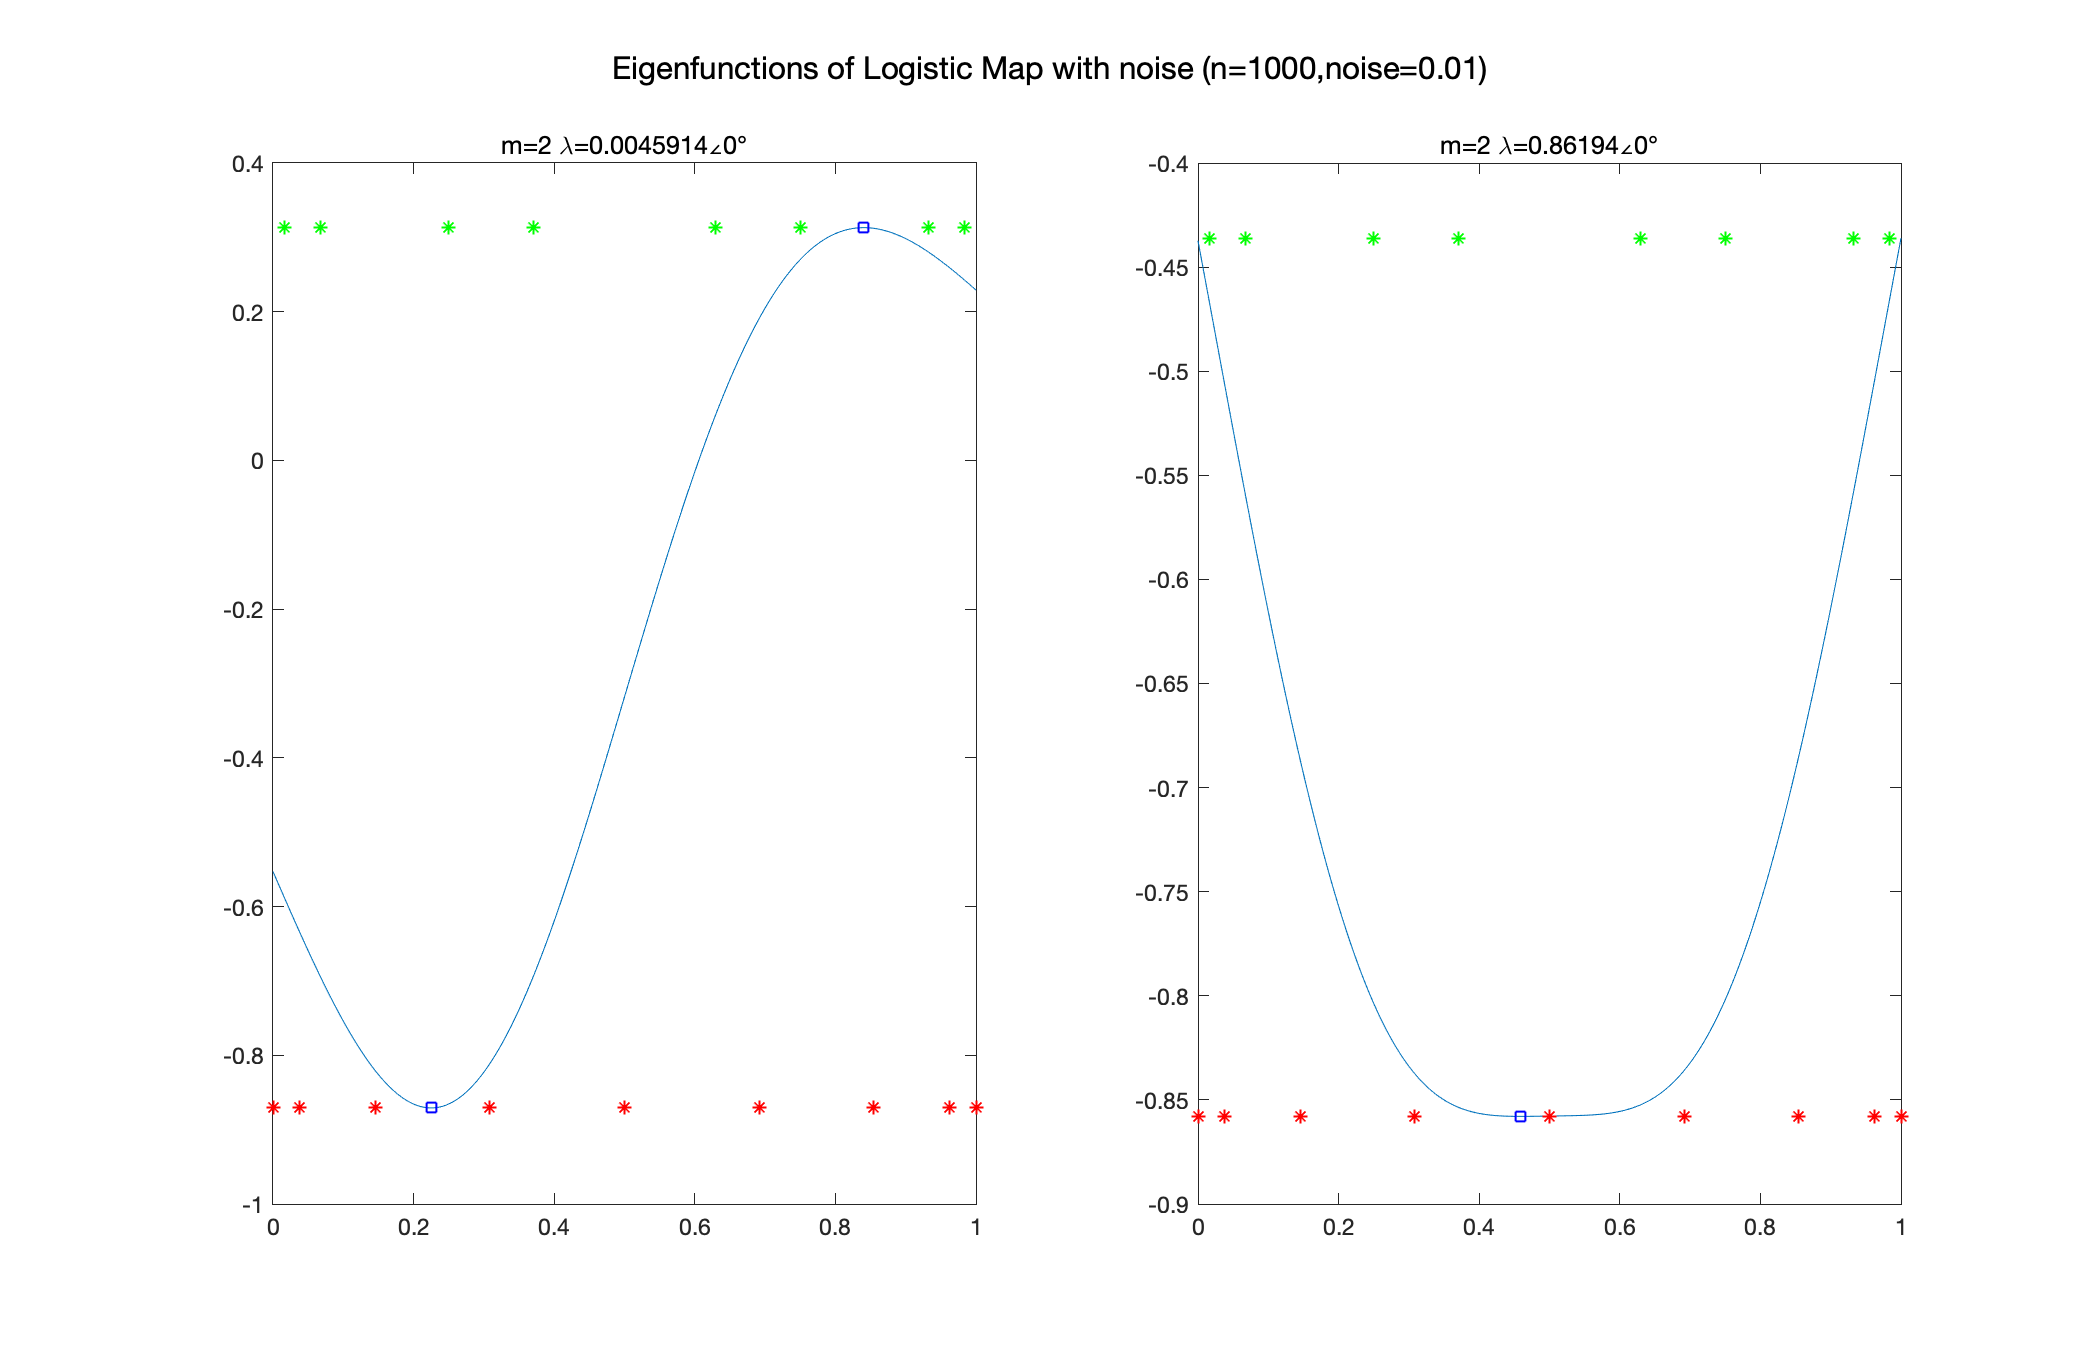
\includegraphics[scale=0.2]{logistic/noise/Logistic_eigen_noise_n1000m2d0-01}}
    \subfloat[m=3]{
      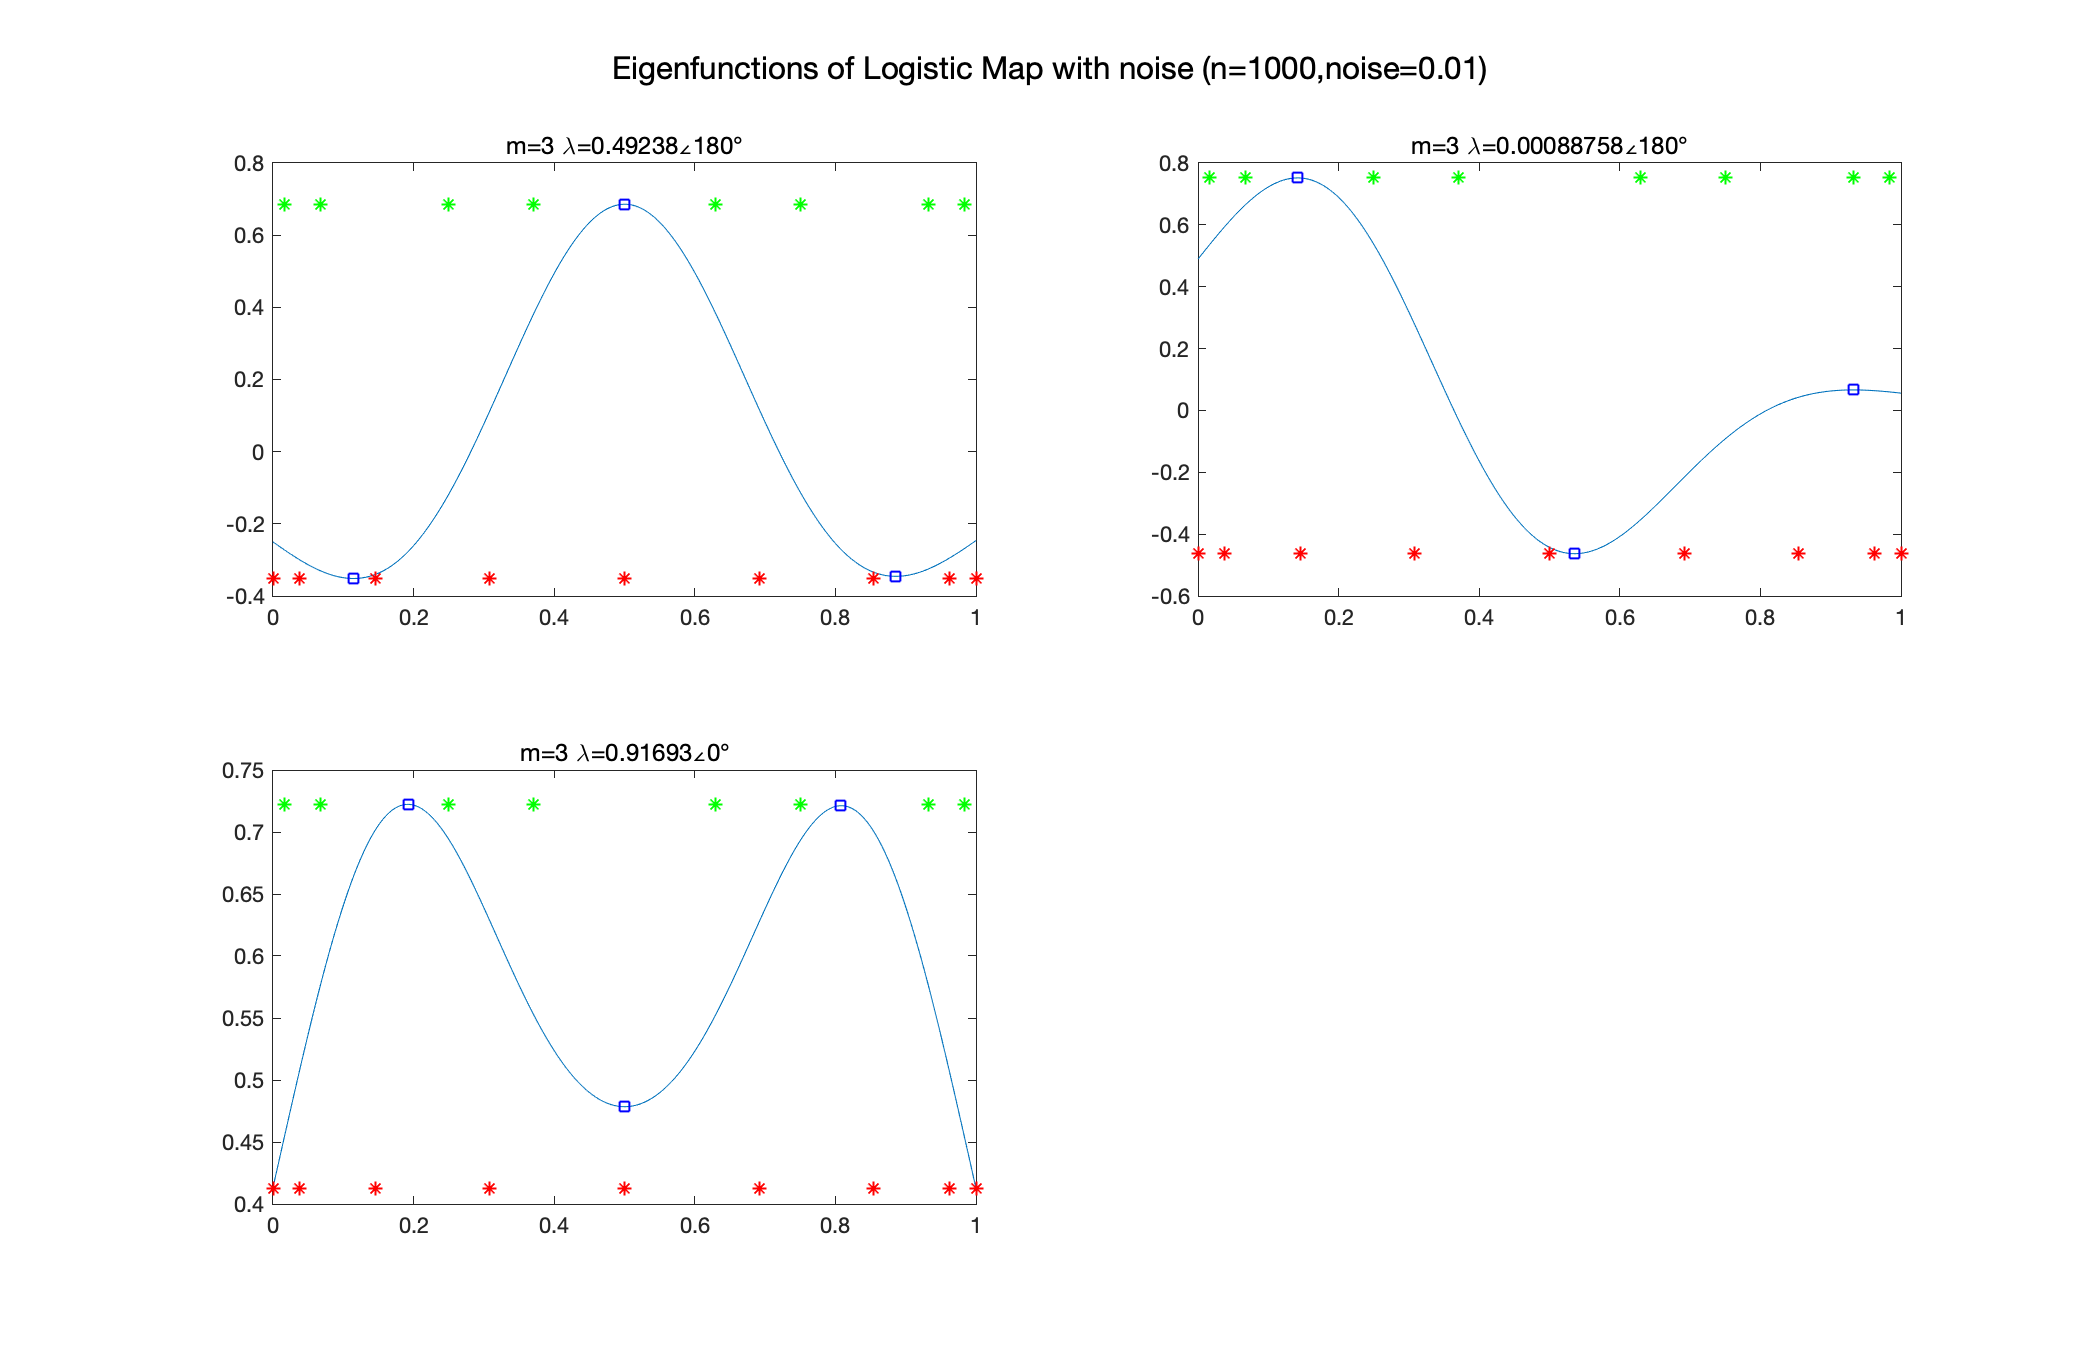
\includegraphics[scale=0.2]{logistic/noise/Logistic_eigen_noise_n1000m3d0-01}}
      \\
    \subfloat[m=4]{
      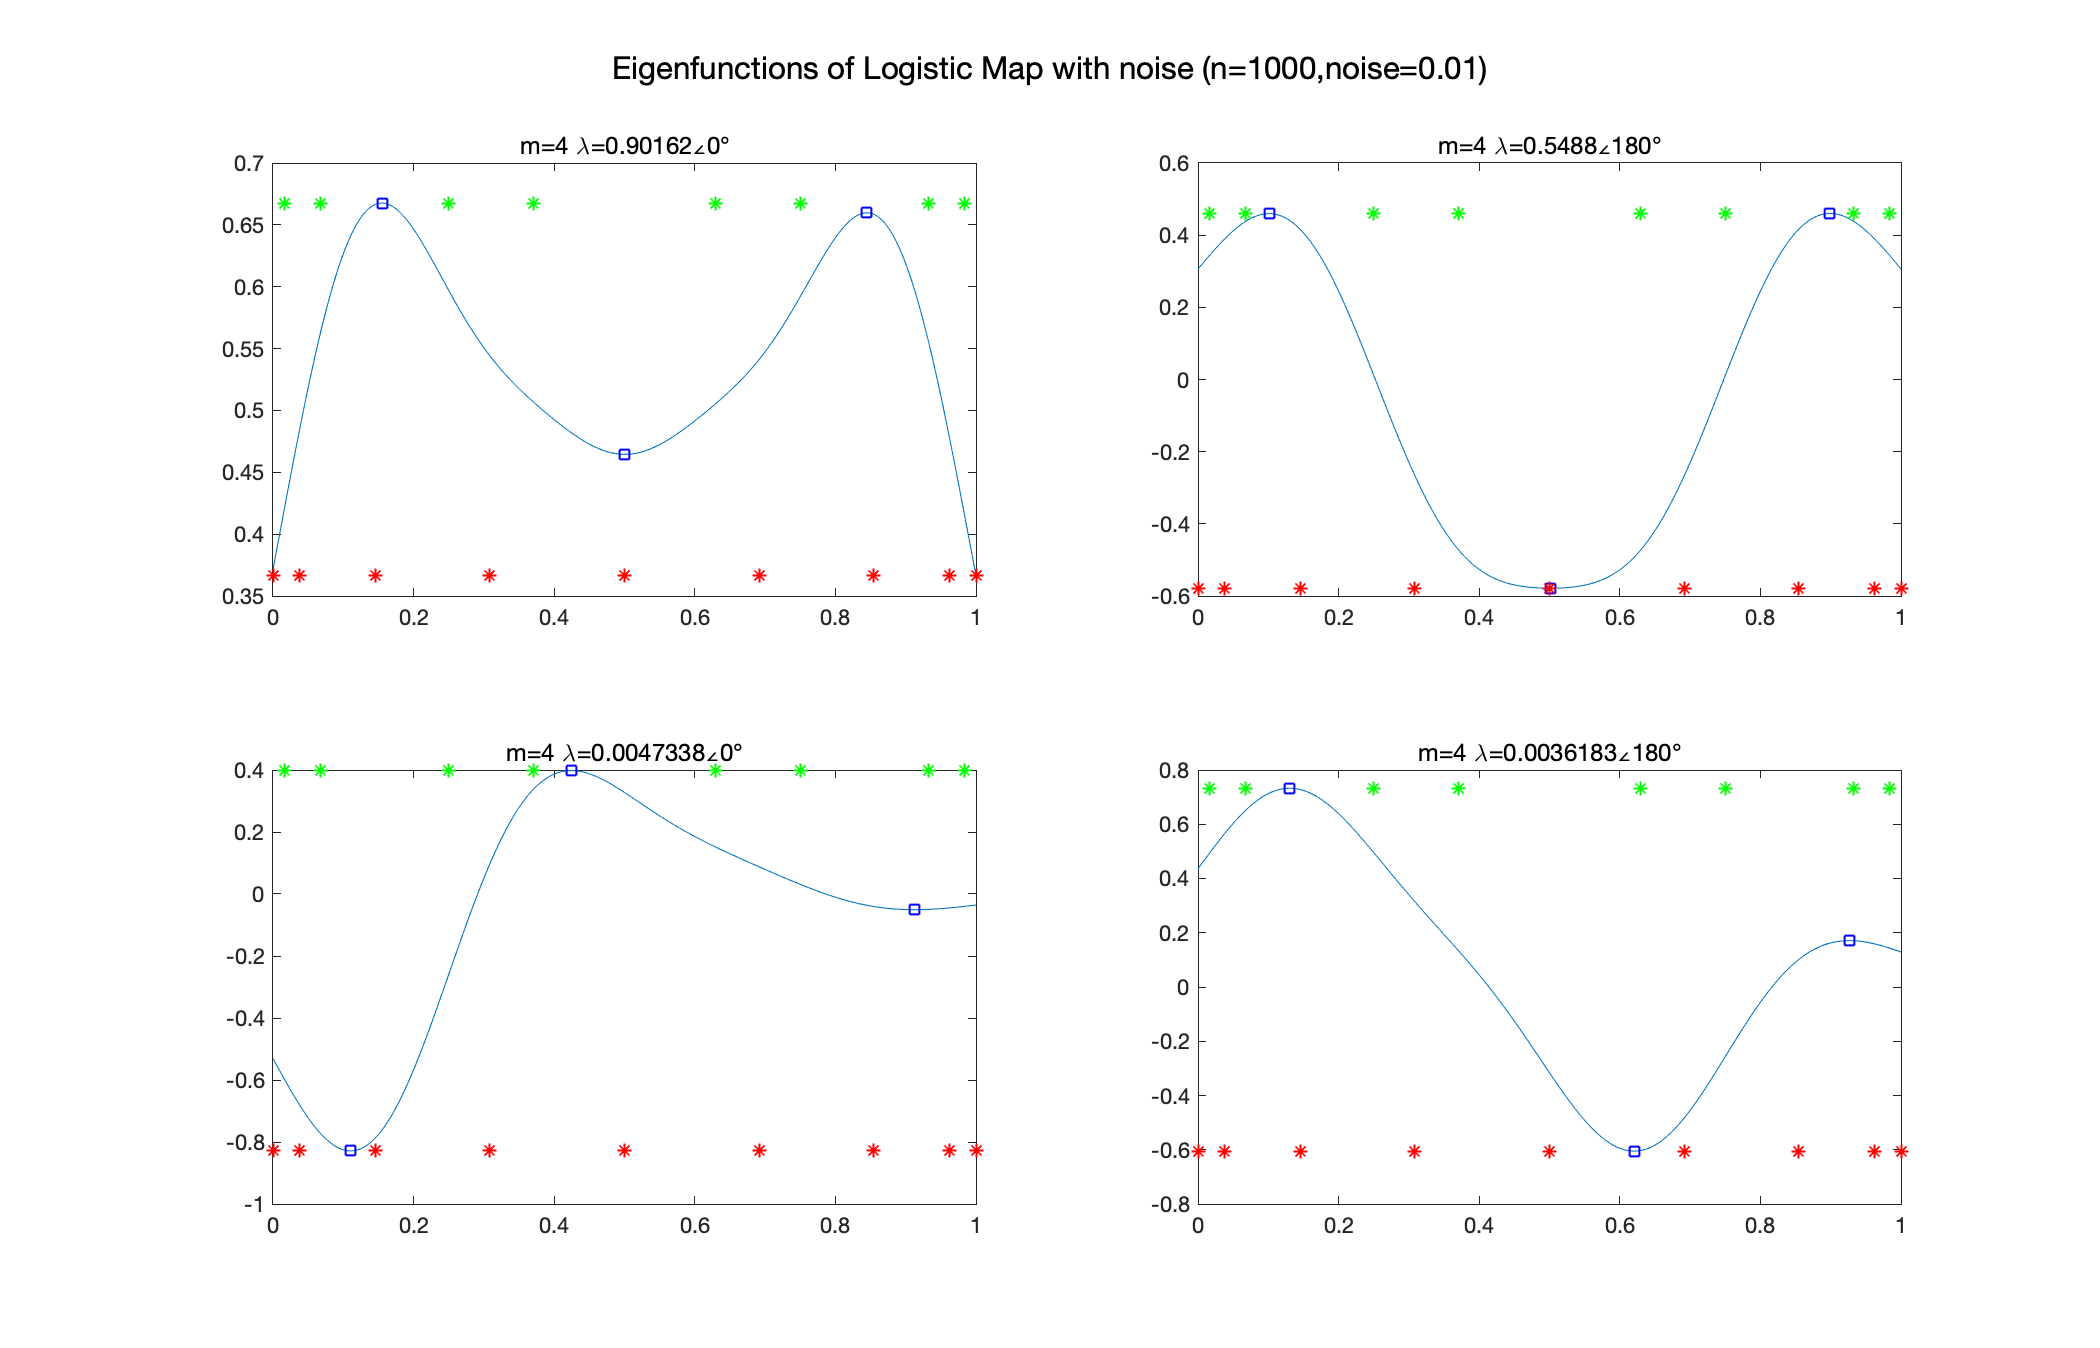
\includegraphics[scale=0.2]{logistic/noise/Logistic_eigen_noise_n1000m4d0-01}}
    \subfloat[m=5]{
      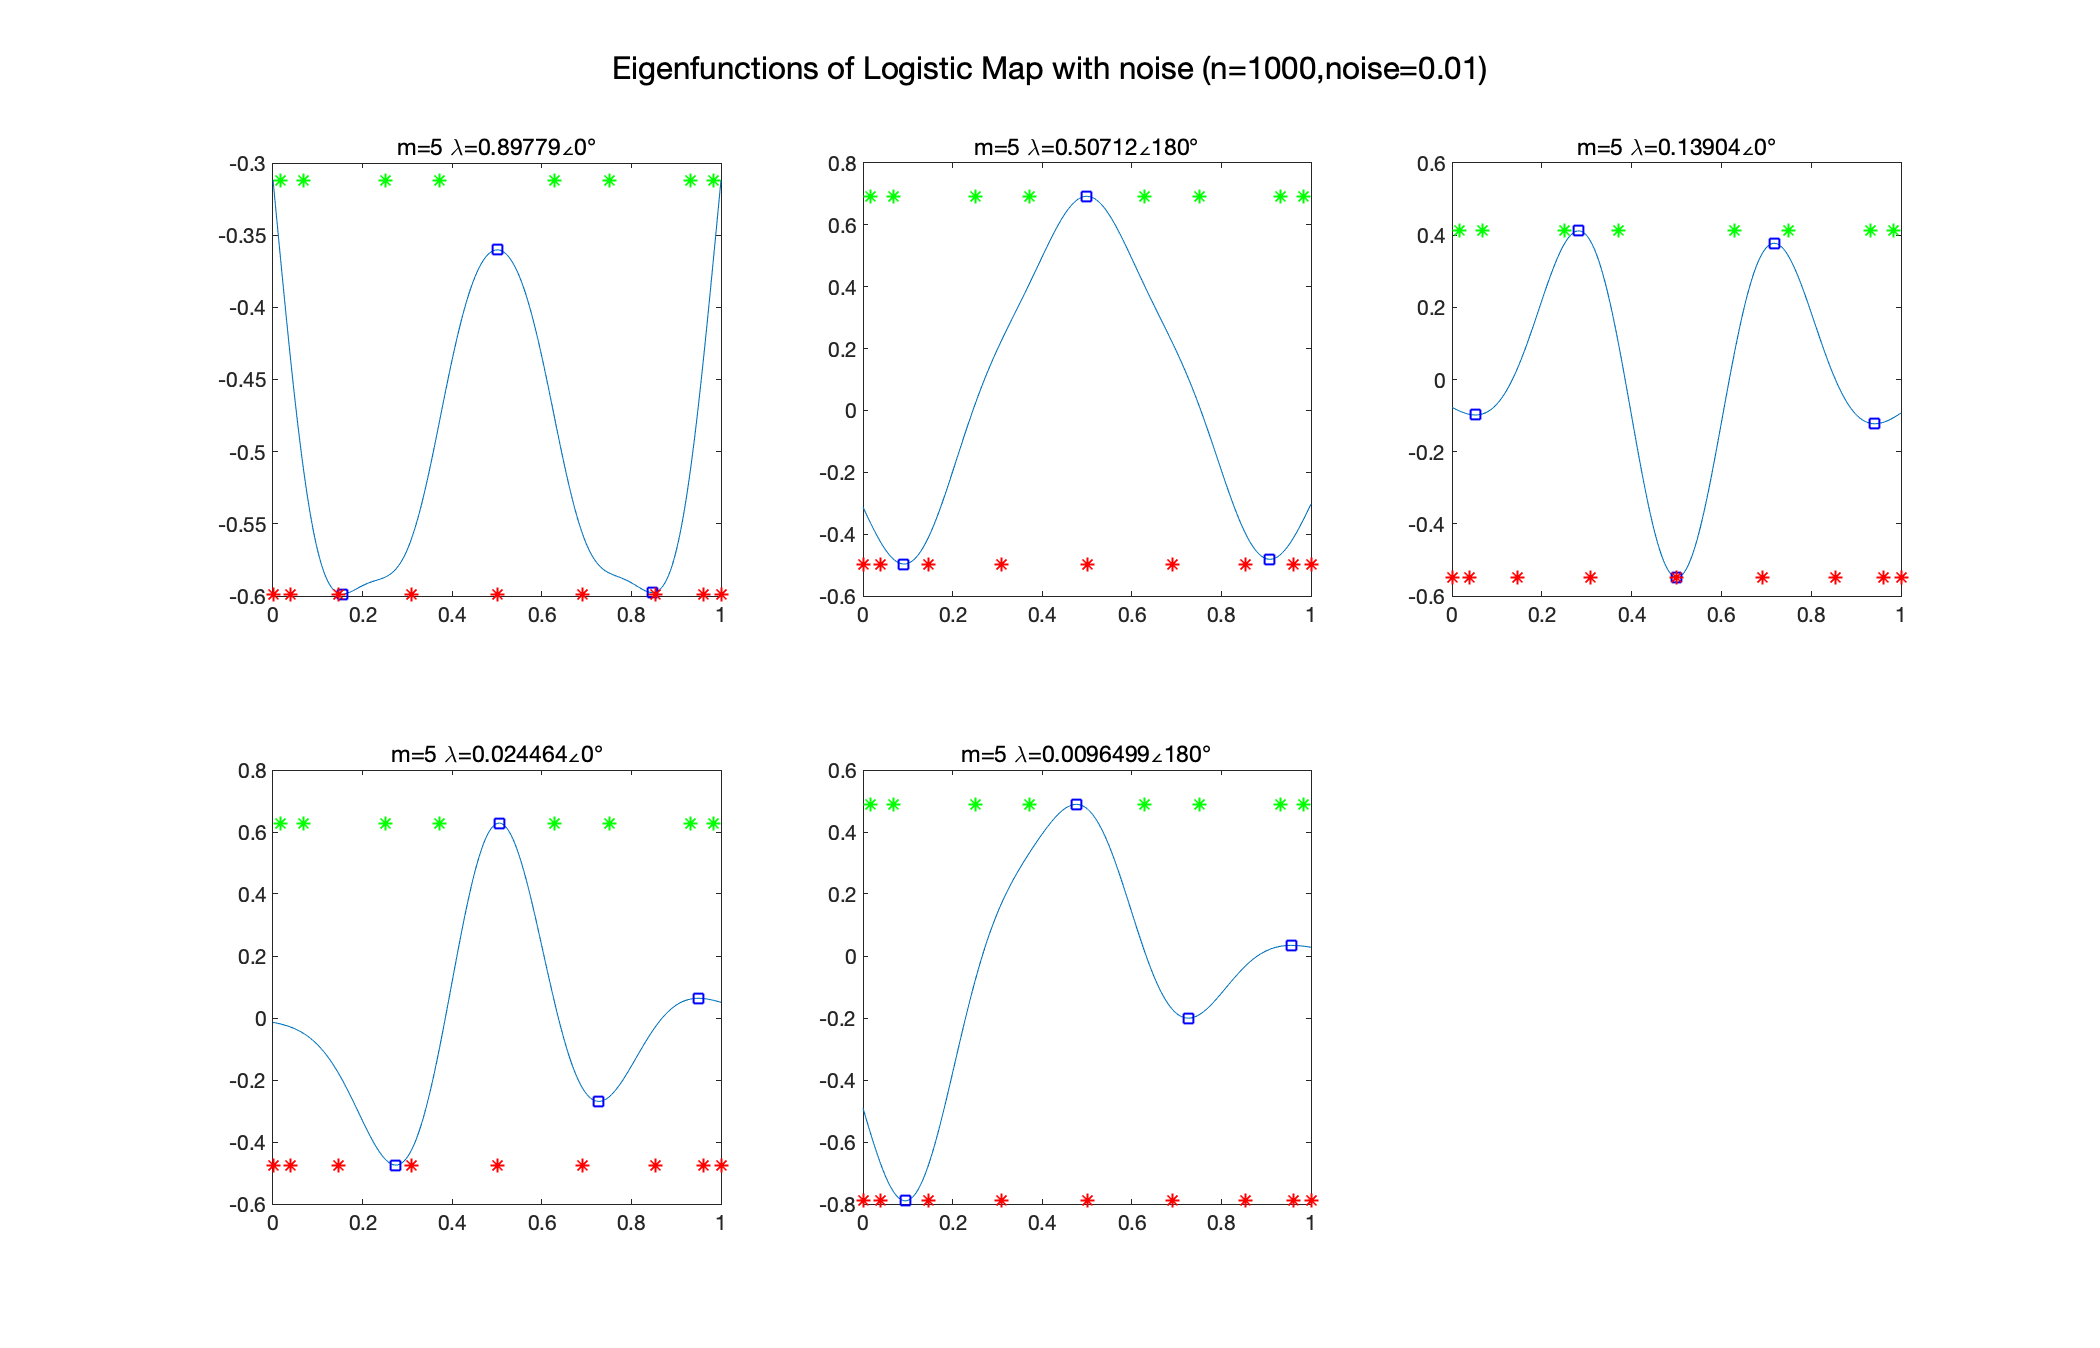
\includegraphics[scale=0.2]{logistic/noise/Logistic_eigen_noise_n1000m5d0-01}}
      \\
    \subfloat[m=8]{
      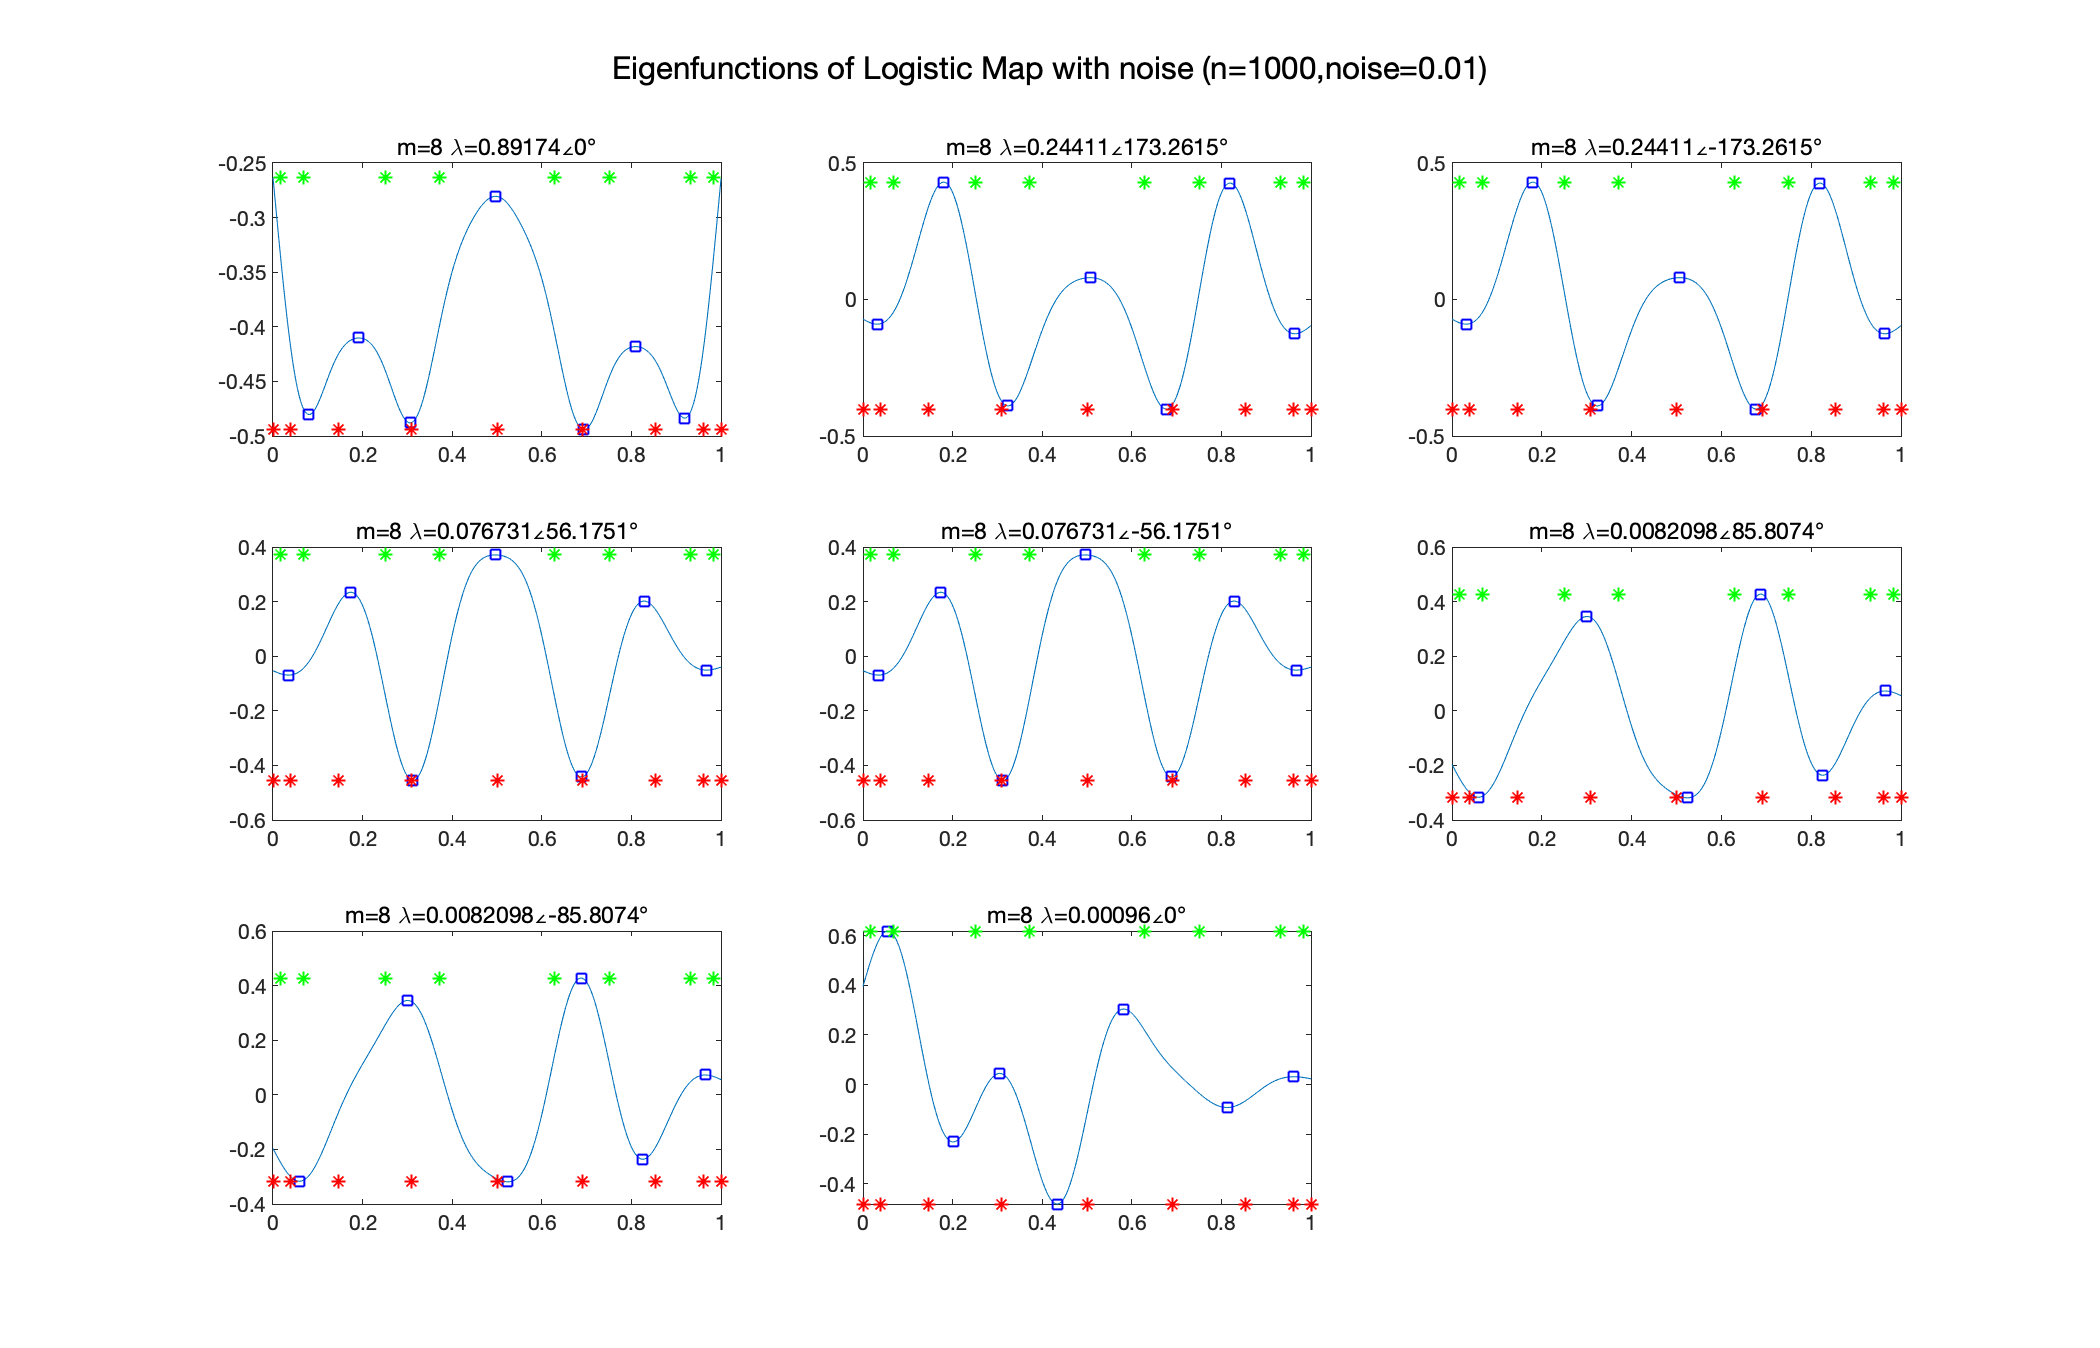
\includegraphics[scale=0.2]{logistic/noise/Logistic_eigen_noise_n1000m8d0-01}}
    \subfloat[m=10]{
      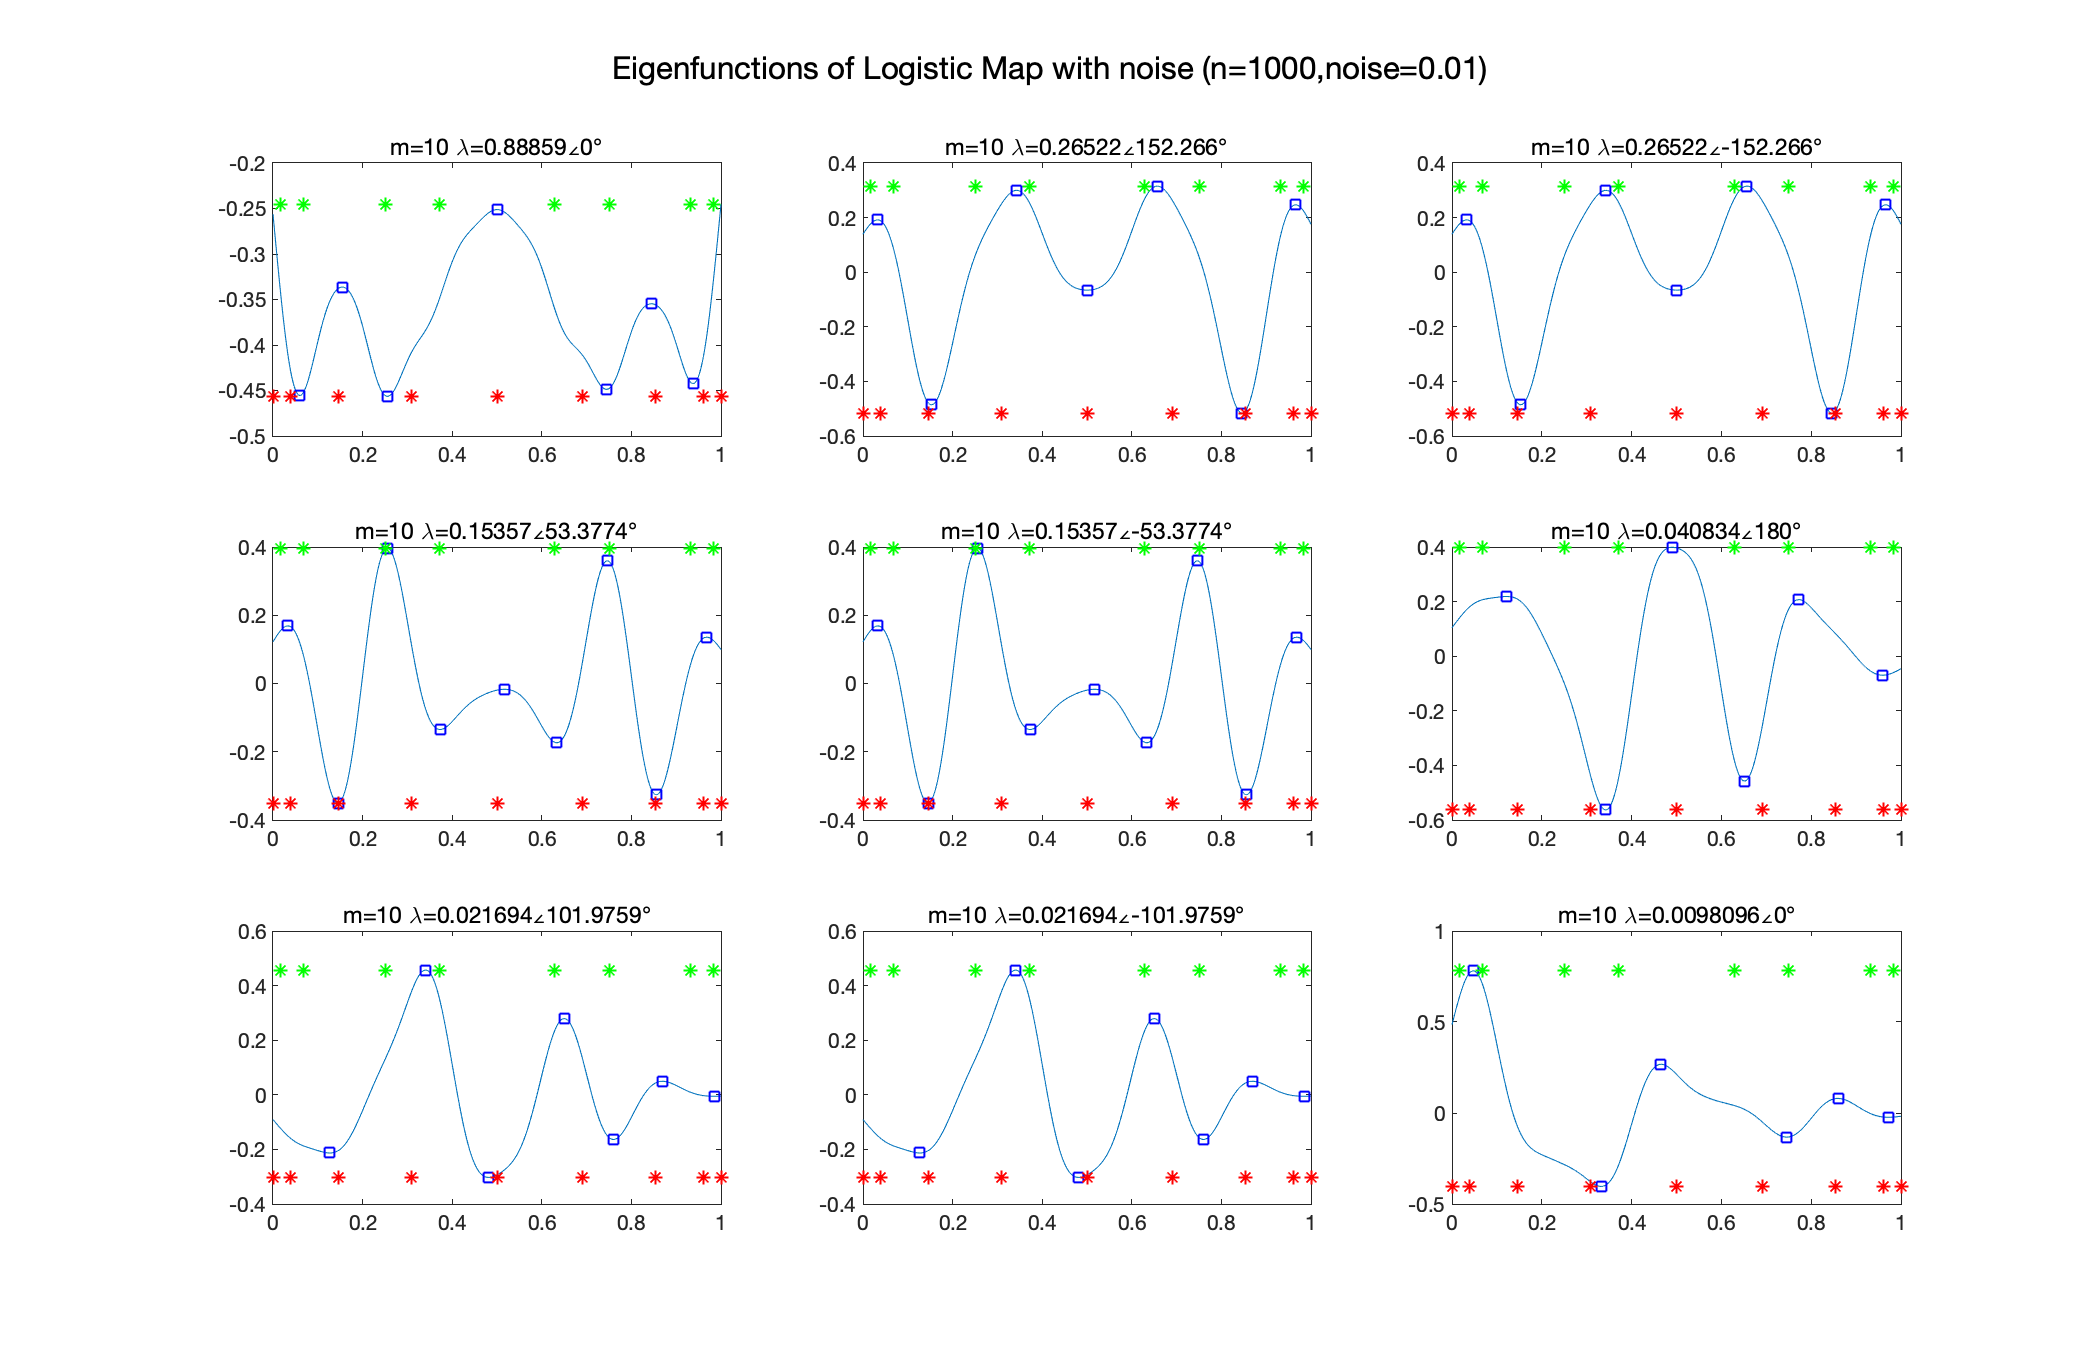
\includegraphics[scale=0.2]{logistic/noise/Logistic_eigen_noise_n1000m10d0-01}}
      \\
    \subfloat[m=15]{
      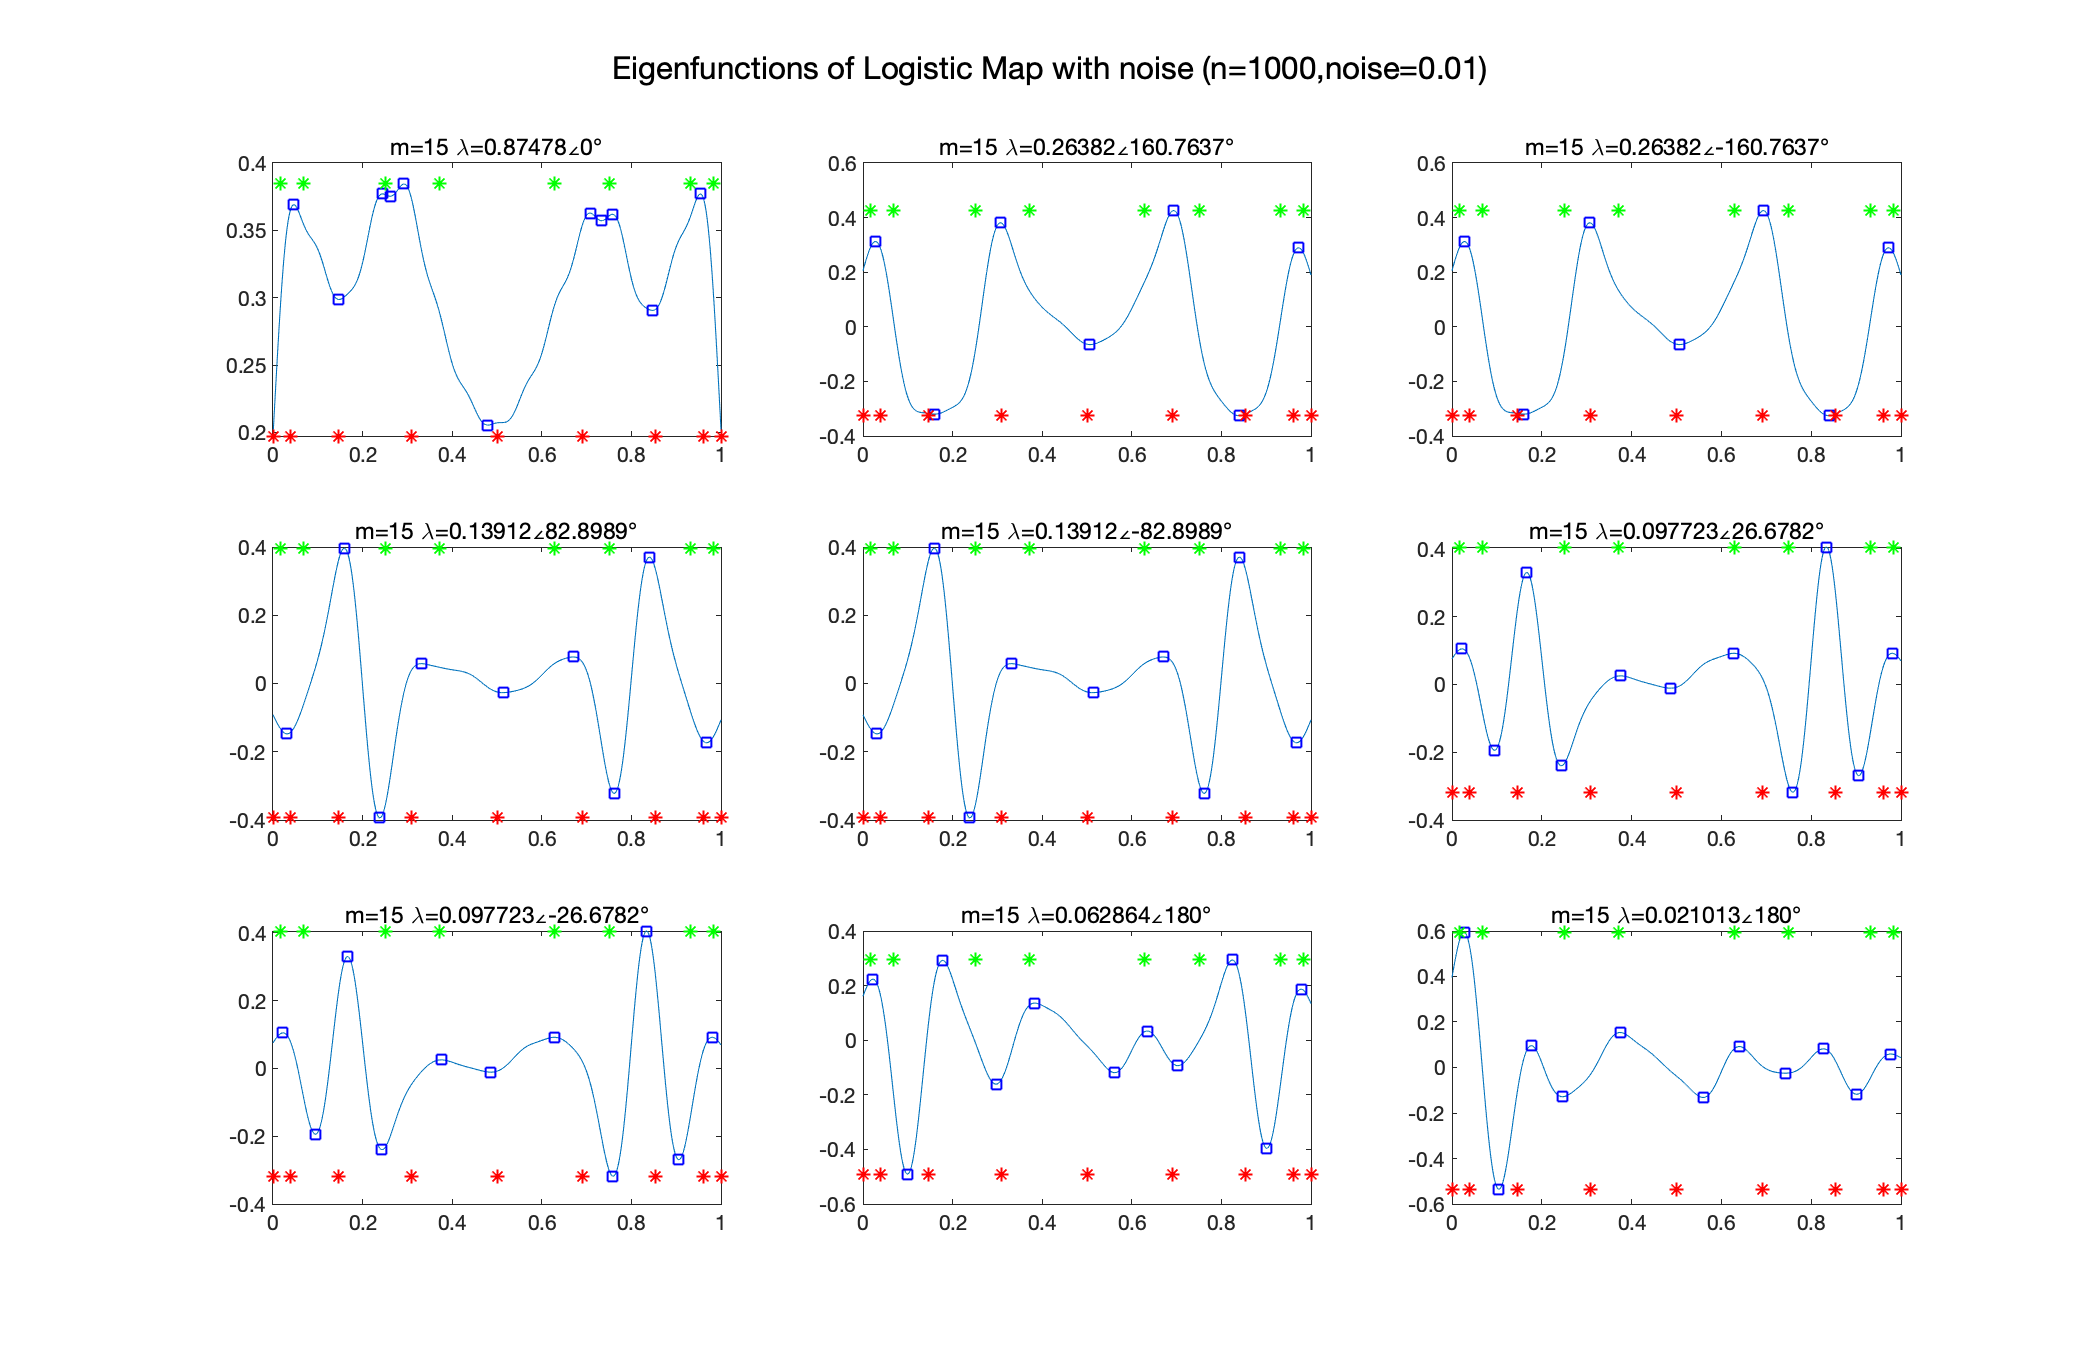
\includegraphics[scale=0.2]{logistic/noise/Logistic_eigen_noise_n1000m15d0-01}}
    \subfloat[m=20]{
      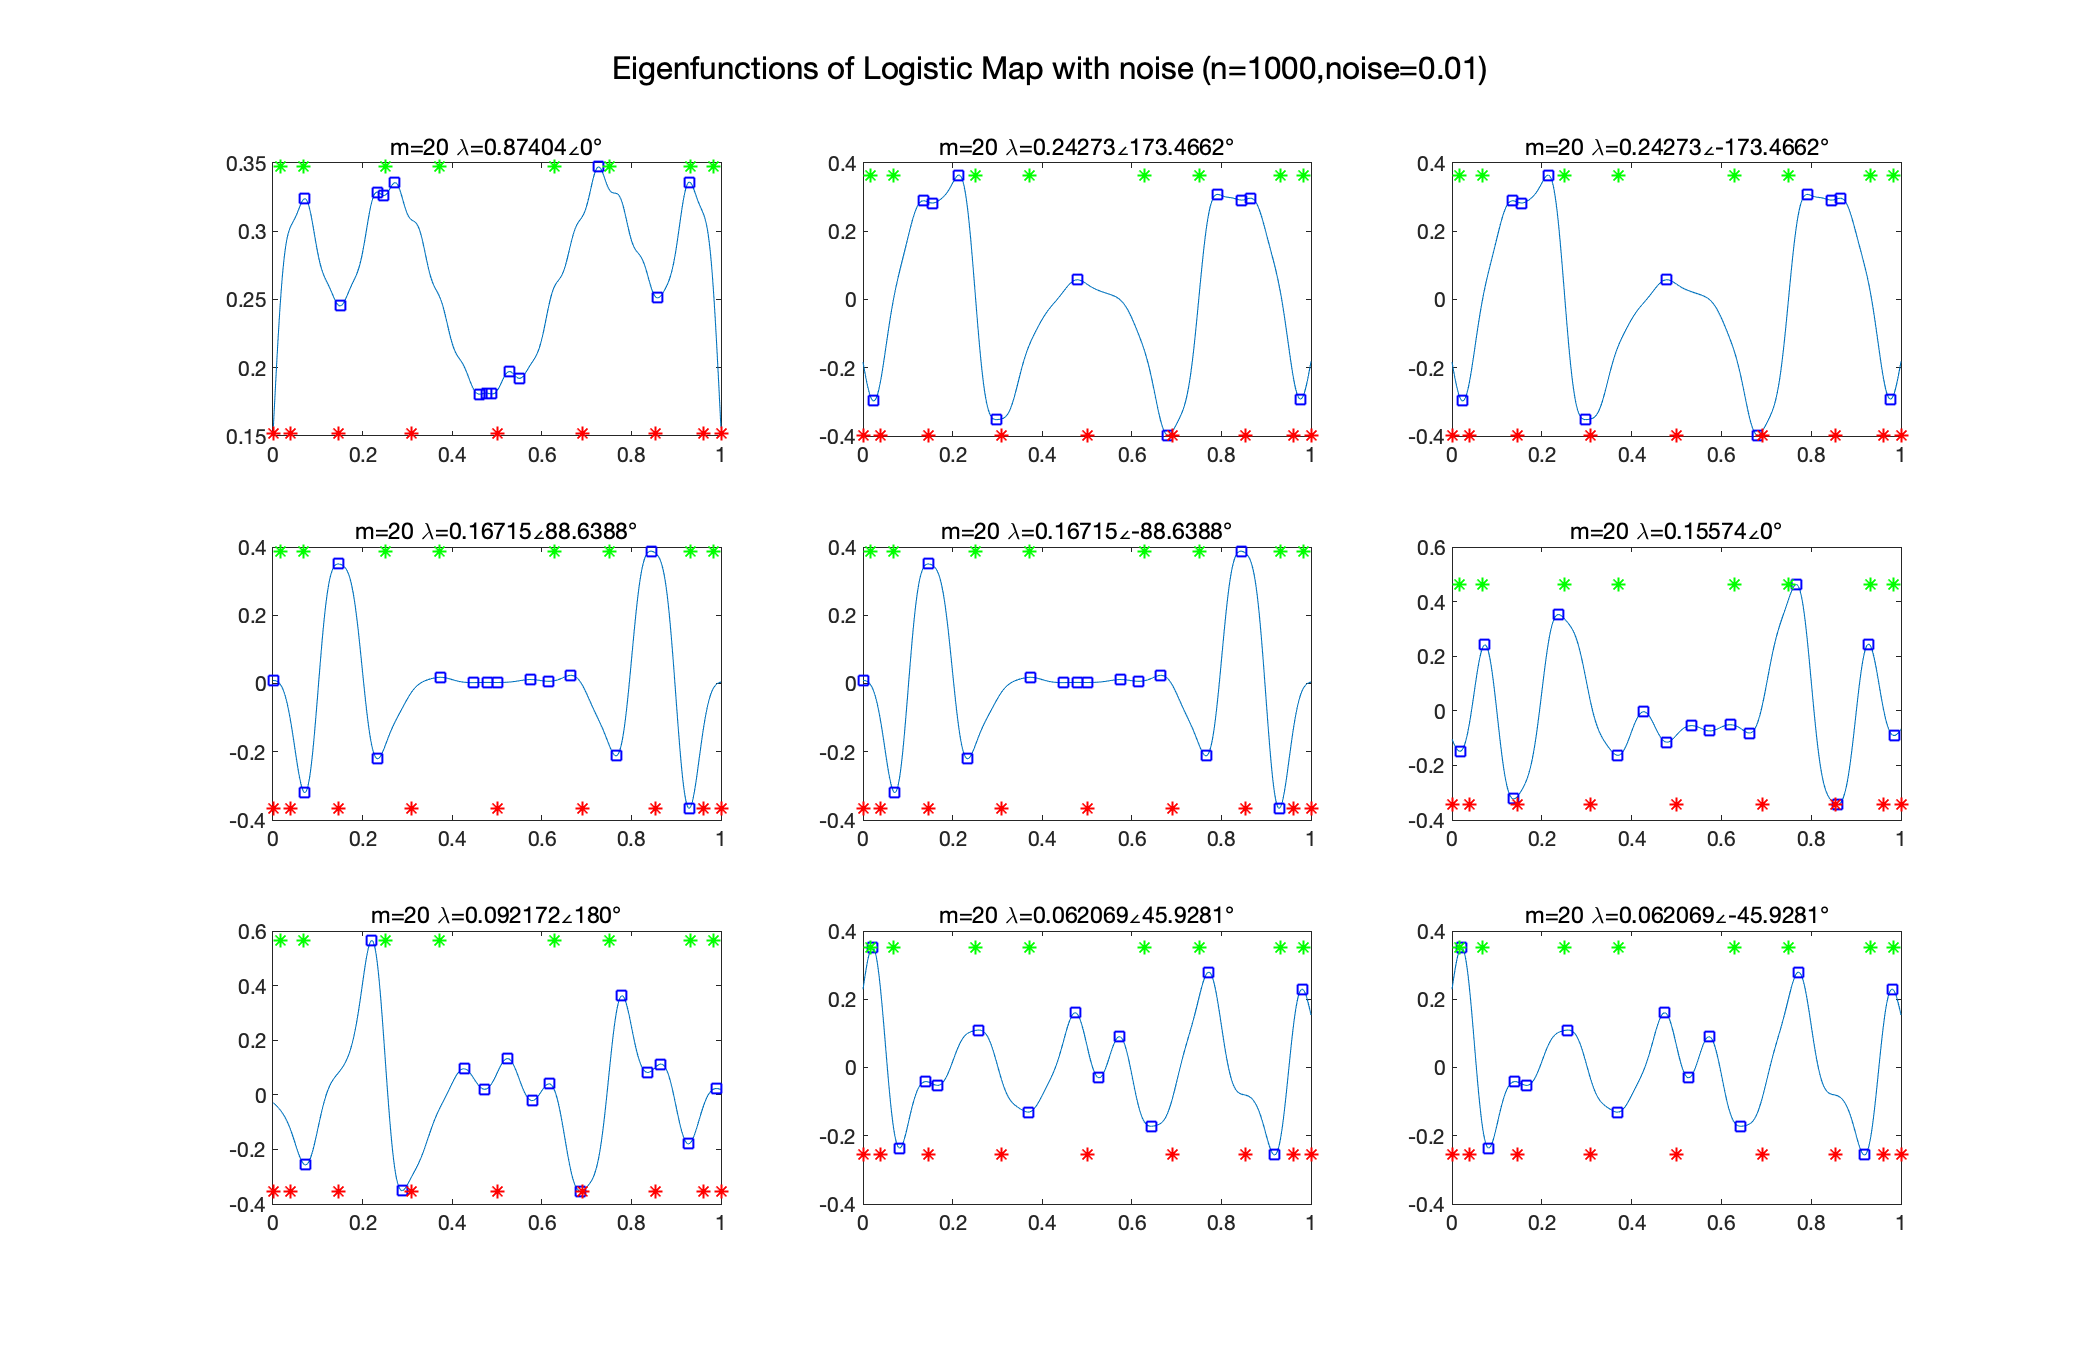
\includegraphics[scale=0.2]{logistic/noise/Logistic_eigen_noise_n1000m20d0-01}}
      \\
      \caption{Logistic映射的边界点与本征函数($noise=0.01$)}
  \end{figure}

\subsubsection{寻找更精确的边界点}

\subsection{小结}


